\documentclass[11pt]{article}

% ==============================================================================
% WORKING PAPER: Productive Capacity as an Institutional Settlement
% Critical Replication and Distributional Extension of Shaikh's Capacity Measure
% Exported from PhD Dissertation source of truth (University of Massachusetts Amherst)
% Mirrored layout engine: Letterpaper, 1.05 stretch, microtype, float auto-scaler
% ==============================================================================

% ---- Language & encoding ----
\usepackage[english]{babel}
\usepackage[T1]{fontenc}
\usepackage{lmodern}

% ---- Layout & Spacing (Dissertation Main Engine) ----
\usepackage[letterpaper, margin=1in]{geometry}
\usepackage{setspace}
\setstretch{1.05}

% ---- Microtypography ----
\usepackage{microtype}

% ---- Math & Theorems ----
\usepackage{amsmath,amssymb,mathtools,bm}
\usepackage{amsthm}
\newtheorem{theorem}{Theorem}
\newtheorem{corollary}{Corollary}

% ---- Figures & Floats ----
\usepackage{graphicx}
\usepackage{float}
\usepackage{placeins}
\usepackage{pdflscape}

% ---- Tables (Dissertation Main Engine) ----
\usepackage{array}
\usepackage{booktabs}
\usepackage{longtable}
\usepackage{tabularx}
\usepackage{makecell}
\usepackage{threeparttable}
\usepackage{siunitx}
\sisetup{group-separator={,}, group-minimum-digits=4}

% ---- Captions ----
\usepackage{caption}
\usepackage{subcaption}
\captionsetup{font=small, labelfont=bf, labelsep=period}

% ---- Lists ----
\usepackage{enumitem}
\setlist{noitemsep, topsep=4pt}

% ---- Math & Text Helpers ----
\usepackage{xfrac}
\usepackage{ragged2e}

% ---- Color Palette ----
\usepackage[dvipsnames]{xcolor}
\colorlet{ink}{black}
\colorlet{subink}{black!72}
\colorlet{lightink}{black!45}
\colorlet{guide}{black!28}
\colorlet{panel}{black!4}
\colorlet{panelb}{black!7}
\colorlet{panelc}{black!10}
\colorlet{stress}{black!12}
\definecolor{navy}{HTML}{1D3557}
\definecolor{crimson}{HTML}{9E2A2B}
\definecolor{amber}{HTML}{E76F51}
\definecolor{darkgreen}{HTML}{2A9D8F}
\definecolor{slate}{HTML}{4A4E69}
\definecolor{darkblue}{rgb}{0,0,0.8}

% ---- TikZ ----
\usepackage{tikz}
\usetikzlibrary{arrows.meta,positioning,calc,matrix}

% ---- Column Types ----
\newcolumntype{L}[1]{>{\raggedright\arraybackslash}p{#1}}
\newcolumntype{C}[1]{>{\centering\arraybackslash}p{#1}}

% ---- Appendix & Bibliography ----
\usepackage{titlesec}
\usepackage[titletoc,toc,title]{appendix}
\usepackage[authoryear]{natbib}

% ---- Hyperref & Cleveref ----
\usepackage[
  colorlinks  = true,
  linkcolor   = darkblue,
  citecolor   = darkblue,
  urlcolor    = darkblue,
  bookmarksnumbered = true,
  pdfauthor   = {Diego Polanco}
]{hyperref}
\usepackage{cleveref}

% ---- Float Autoscaler Hook (Mirrored from Dissertation Main integration) ----
% Dynamically rescales completed floats only when exceeding text height,
% guaranteeing that large tables and stacked panels fit on a single page.
\newsavebox{\WorkingPaperFloatBox}
\makeatletter
\let\wp@endfloatbox\@endfloatbox
\def\@endfloatbox{%
  \wp@endfloatbox
  \ifdim\dimexpr\ht\@currbox+\dp\@currbox\relax>\textheight
    \typeout{WORKING PAPER: fitting oversized float to page height}%
    \setbox\WorkingPaperFloatBox\box\@currbox
    \global\setbox\@currbox\vbox{%
      \hbox to\columnwidth{\hfil
        \resizebox*{!}{0.98\textheight}{\usebox{\WorkingPaperFloatBox}}%
      \hfil}}%
  \fi
}
\makeatother

% ---- Paragraph Rhythm ----
\setlength{\parskip}{0.55em}
\setlength{\parindent}{0pt}

% ---- Graphicspath ----
\graphicspath{{figures/}{appendixA/figures/}{../../Chapter1/figures/}{../../Chapter1/appendixA/figures/}}

% ---- Working Paper Metadata ----
\title{\textbf{Replicating Shaikh's Capacity Utilization Measure: Specification Sensitivity and Distribution}\thanks{Doctoral Candidate in Economics, Department of Economics, University of Massachusetts Amherst. Email: \texttt{dpolanconeco@umass.edu}. This working paper draws upon and extends research from the author's doctoral dissertation at the University of Massachusetts Amherst. The author thanks the dissertation committee members for invaluable comments and guidance. All analytical arguments, empirical results, and remaining errors are the author's sole responsibility.}}

\author{\textbf{Diego Polanco}\thanks{Department of Economics, University of Massachusetts Amherst.} \\
Department of Economics, University of Massachusetts Amherst}

\date{October 2026 \\ \vspace{0.5em} \small\textbf{Working Paper}}

\begin{document}

\maketitle

\begin{abstract}
This paper critically replicates Anwar Shaikh's (2016) capacity utilization measure for the post-war US corporate sector (1947--2011), evaluating the long-run output--capital coefficient as a capacity transformation elasticity ($\theta$). A faithful single-equation ARDL reconstruction reproduces the baseline parameter within canonical data bounds ($\hat{\theta} \approx 0.72$). However, expanding the specification space across a 500-model ARDL lattice reveals substantial sensitivity (with $\hat{\theta} \in [0.65, 0.95]$ among retained no-trend specifications, while trend-containing models reach 2.20), demonstrating that single-equation capacity paths are non-unique. Moving to a system framework, across 48 attempted bivariate VECM specifications, 36 are successfully estimated, and none of those 36 identifies an admissible cointegrating relation. Within the tested full-sample system grid, long-run system stability becomes recoverable only when the rate of exploitation enters the state vector alongside historical shock controls. In the focal trivariate VECM, the exploitation parameter is identified with high precision, yielding a focal elasticity point estimate of $\hat{\theta} \approx 0.73$ alongside substantial estimation uncertainty. Productive capacity is therefore not an insulated engineering constant, but a macro-structural outcome conditioned by institutional settlements governing distribution.
\end{abstract}

\vspace{0.8em}
\noindent\textbf{Keywords:} Capacity Utilization, Critical Replication, Transformation Elasticity, Cointegration, ARDL, VECM, Distributional Conflict, Exploitation Rate.

\vspace{0.4em}
\noindent\textbf{JEL Codes:} B51, C32, E01, E22, E32, P16.

\clearpage

% ── Manuscript Sections ────────────────────────────────────────────────────────
\section{Introduction}
\label{sec:introduction}

Measuring productive capacity is fundamental to macroeconomic theory, yet capacity output is unobservable. Conventional output-gap and survey measures impose strong cyclical or technical assumptions, often conflating engineering limits with demand fluctuations. \citet{Shaikh2016} proposes an influential alternative: an accounting-based measure derived from a long-run cointegrating regression between aggregate output and capital stock in the US corporate sector (1947--2011). Shaikh interprets the resulting long-run coefficient as an empirical anchor for potential output and treats the residuals as cyclical capacity utilization. This paper critically replicates Shaikh's empirical procedure to evaluate whether the estimated output--capital relation represents a stable technical benchmark or a specification-sensitive artifact.

To evaluate this relation, I reframe the aggregate output--capital coefficient as a capacity transformation elasticity ($\theta \equiv \partial \ln Y^p / \partial \ln K$). Under the balanced-growth knife-edge assumption standard in post-Keynesian models, this elasticity is constrained to unity ($\theta = 1.0$), meaning productive capacity expands in lockstep with capital accumulation. When $\theta \neq 1.0$, however, capacity formation decouples from accumulation: an elasticity below unity ($\theta < 1.0$) defines structural overaccumulation, where capital accumulates faster than capacity expands, while $\theta > 1.0$ generates chronic excess capacity. Reconstructing Shaikh's single-equation ARDL(2,4) baseline (Stage S0) demonstrates that the estimation is approximately reproducible within canonical data bounds ($\hat{\theta} \approx 0.72$ versus Shaikh's published 0.66), yielding a point estimate within the structural overaccumulation interval.

Yet this baseline point estimate is fragile across model choices. In Stage S1, I evaluate a combinatorial grid of 500 ARDL specifications varying lag lengths, deterministic trends, and structural break subsets. While 102 specifications satisfy the baseline $F$-bounds test at the 10\,\% level (and 62 at the 5\,\% level), the recovered transformation elasticity varies widely across the informational frontier ($\hat{\theta} \in [0.65, 0.95]$). Rather than converging to a unique technical constant, the single-equation framework exhibits disciplined non-uniqueness: the estimated capacity ceiling depends substantially on researcher choices regarding lag profiles and deterministic terms.

Moving from single-equation regressions to a joint system framework reveals a deeper econometric limitation. In Stage S2, I evaluate 48 attempted bivariate Vector Error Correction Models (VECMs, of which 36 are successfully estimated) sweeping lag orders and deterministic configurations over the 1947--2011 sample. The standalone bivariate output--capital relation fails to cointegrate in every tested specification. Residuals exhibit persistent non-stationary drift. Aggregate output and capital stock do not form an empirically self-sufficient cointegrating system in isolation over the post-war period.

Long-run system stability becomes recoverable only when the rate of exploitation enters the state vector alongside historical shock controls. In a trivariate VECM $(\ln Y, \ln K, \ln e)$, where $\ln e_t = \ln \pi_t - \ln \omega_t$ captures functional income distribution, six specifications achieve cointegration rank $r=1$ and companion matrix stability. In the focal model, the estimated elasticity point estimate ($\hat{\theta} = 0.727$) sits in the overaccumulation range, but carries substantial normalized estimation uncertainty ($\text{SE} = 4.852, t = -0.15$). In sharp contrast, the coefficient on the rate of exploitation is identified with high precision ($\hat{\beta}_e = 20.022, \text{SE} = 2.536, t = 7.90$). The system demonstrates that functional distribution enters the long-run attractor with dominant statistical significance, while the transformation elasticity remains imprecisely estimated once unconstrained by single-equation assumptions.

These empirical findings motivate a conceptual reinterpretation of capacity formation. The output--capital relation does not fail because capital is unproductive; rather, productive capacity is distributionally conditioned. In capitalist economies, converting capital equipment into potential output depends on the intensity of the labor process, work organization, and shift arrangements. These parameters are not neutral engineering constraints. They are structured by the distribution of income between profits and wages and the institutional settlements that govern the workplace. System stability emerges only when the econometric model incorporates the distributional mechanisms through which capital accumulation is socially coordinated and disciplined.

The remainder of the paper proceeds as follows. Section~\ref{sec:literature_review} traces the historical shift in capacity utilization metrics from engineering surveys to cyclical disciplining tools. Section~\ref{sec:conceptual_framework} develops the conceptual framework, formalizing the transformation elasticity and its connection to Marxian profit rate decompositions and choice-of-technique dynamics. Section~\ref{sec:replication_strategy} presents the three-stage econometric results: single-equation reconstruction (S0), specification geometry across the ARDL lattice (S1), and system-level VECM estimation (S2). Section~\ref{sec:discussion} discusses the theoretical implications of structural overaccumulation, the institutional interpretation of distributional conditioning, and methodological boundaries. Section~\ref{sec:conclusion} concludes.

\section{A Historical Trace of Capacity Utilization Measurement}
\label{sec:literature_review}

This section traces the evolution of capacity utilization measurement from early industrial surveys to contemporary output-gap governance. The metric originally emerged to quantify idle capital during the Great Depression, shifted toward inflation surveillance during the stagflation crisis of the 1970s, and now informs technocratic output-gap benchmarks. Throughout these phases, the unobserved productive ceiling has remained conceptually underidentified. I trace this trajectory through four developments: the standardization of survey measures during the Fordist era, the transition to output-gap governance, the theoretical debates between Sraffian and Kaleckian economists over long-run utilization, and Shaikh's accounting-based framework.

\subsection{From Survey Measures to an Inflation Sentinel: Capacity Utilization during the Fordist Era}
\label{subsec:fordist_survey_statecraft}

Before capacity utilization could serve as a policy benchmark, researchers had to confront a conceptual divergence in its definition. The mass idleness of the Great Depression forced statistical agencies to quantify unused resources, exposing an enduring tension between engineering and economic definitions of productive capacity \citep{Burns1954, KleinDavid1958}. Engineering capacity represents the physical ceiling of machine operation under uninterrupted conditions. Economic capacity, by contrast, defines the profit-maximizing level of output given prevailing wages, input costs, and operating schedules. Early measurement initiatives focused on determining normal operating rates for enterprises amidst the emergence of post-Depression macroeconomic policy.

During the post-war expansion, Alvin Hansen's stagnation thesis warned that chronic underutilization of capital posed an enduring drag on long-run growth \citep{Hansen1936, Hansen1941, Barber1987}. As the neoclassical synthesis codified these concerns into IS-LM demand management \citep{Hicks1937, Samuelson1947, Samuelson1948}, quantitative indicators were required to detect bottlenecks and effective-demand shortfalls. Capacity utilization emerged as a primary metric to render capital idleness legible for countercyclical stabilization.

The McGraw-Hill plant-and-equipment surveys standardized this reporting by asking plant managers to state their operating rates relative to preferred benchmarks. Emerging from the private sector, these surveys served corporate planning and business forecasting before public initiatives took root \citep{BaranSweezy1988, Munroe2007, Butler1958, Phillips1963}. By aggregating firm-level responses into a standardized statistical index, the surveys offered a consistent language for business forecasting. When the Federal Reserve Board subsequently integrated these survey responses into its official Industrial Production index, managerial assessments became an institutional benchmark for macroeconomic surveillance \citep{Board2017}. Alternative physical indicators---such as the workweek of capital \citep{Foss1963, TaubmanGottschalk1971}---never secured comparable bureaucratic adoption.

The stagflation crisis of the 1970s dismantled the post-war demand-stabilization framework. Faced with falling profit rates and rising inflation, policymakers repurposed the capacity index: it functioned less as an indicator of effective-demand shortfalls to be expanded, and more as a sentinel for inflation control \citep{ShaikhManiatisPetralias1999}. High capacity utilization was treated as a warning of impending price pressures, prompting monetary tightening. Academic and policy discussions increasingly evaluated capacity measures by their ability to predict inflation \citep{KleinEtAl1973}. In these debates, Alan Greenspan argued that capacity measures must reflect systemic shortages rather than administrative averages, asserting that ``if the numbers do not indicate that the economy is currently at capacity, then I suggest that the numbers are wrong, and that the correct concept of capacity must reflect the situation'' \citep[p.~758]{KleinEtAl1973}. This shift established the conceptual foundation for modern output-gap governance.

\subsection{From Capacity Utilization to Output-Gap Governance}
\label{subsec:output_gap_governance}

During the late twentieth century, the growth of international trade and financial integration reduced the policy primacy of national manufacturing surveys. Central banks and international agencies turned toward portable, rule-based indicators to monitor macroeconomic conditions \citep{Jessop2002, Jessop2003, Konings2007}. This shift elevated the ``output gap''---the difference between actual and potential output---as the core operational anchor for monetary frameworks, including inflation targeting and Taylor rules \citep{Taylor1993, Johnson2024}. Under the New Consensus Macroeconomics, potential output was defined as the non-accelerating inflation limit of economic activity, often linked to NAIRU benchmarks \citep{SaadFilho2018}. Yet potential output remained an unobservable latent variable whose trajectory depends heavily on statistical filtering choices \citep{HerndonAshPollin2014, AshBasuDube2017}.

Because potential output cannot be observed directly, its estimation depends on specific modeling assumptions. Mainstream practice typically relies on statistical filters that smooth observed output \citep{HodrickPrescott1997, BaxterKing1999, BeveridgeNelson1981, Hamilton2018}, aggregate production functions \citep{CBO2004PotentialGDP, Alichi2015}, or structural vector autoregressions \citep{BlanchardQuah1989}. These methodologies treat potential output as a frictionless trend or an engineering trajectory. In political economy, by contrast, the conversion of productive equipment into realized output is understood as institutionally mediated. At the plant level, work schedules, line speeds, and labor discipline govern how intensively physical equipment can run. In the macroeconomy, the realization of potential output interacts with distributive conflict, reserve-army dynamics, and profitability. When low unemployment strengthens labor's bargaining position, resulting profit-squeeze pressures may lead firms to idle capacity rather than expand production. Distinguishing between physical equipment and institutional conditions is therefore central to measuring the capacity ceiling.

The 2008 Global Financial Crisis exposed the practical limits of this filtering approach. Post-crisis revisions routinely altered the sign of estimated output gaps, and downward revisions to potential output were used to justify fiscal austerity in the European periphery \citep{Heimberger2017, Heimberger2020}. Although international institutions documented substantial hysteresis and revision volatility \citep{CerraSaxena2017, CerraFatasSaxena2023}, surveillance frameworks continued to rely on output-gap calculations for real-time policy guidance \citep{AastveitTrovik2014, Foster2024}. This revision-prone setting provides the institutional context for heterodox alternatives to capacity measurement.

\subsection{Capacity-Utilization Debates in Political Economy}
\label{subsec:pe_utilization_debates}

Within political economy, the ``capacity utilization controversy'' divides scholars along a central question: is the long-run normal rate of utilization endogenous to demand, or is it anchored in cost structures and classical competition? The Neo-Kaleckian tradition treats the normal rate as endogenous, arguing that firms adjust long-run operating rates in response to demand shocks, shift choices, or historical hysteresis \citep{Lavoie1995, Nikiforos2013, Setterfield2020}. In contrast, Sraffian economists argue that cost minimization and classical competition anchor the normal rate of utilization in the long run, with capital investment adjusting capacity to meet changes in effective demand \citep{Ciccone1986, Kurz1986}.

Both positions face empirical and conceptual challenges when identifying the productive ceiling. In the Sraffian supermultiplier framework, convergence to a normal rate requires an autonomous component of demand, a condition that can generate tensions with the debt dynamics of stock-flow consistent models \citep{Nikiforos2018}. Conversely, the Neo-Kaleckian hypothesis of endogenous utilization requires capacity utilization to exhibit long-run non-stationarity. Empirical tests of this hypothesis remain contested: \citet{GahnGonzalez2020, GahnGonzalez2022} argue that capacity utilization is stationary and mean-reverting, whereas \citet{Nikiforos2020} shows that unit-root inferences depend on sample selection and deterministic specifications.

Furthermore, by focusing primarily on manufacturing, both the FRB and alternative survey series miss the broader structural shifts of modern, service-dominated economies \citep{Haluska2023}. Evaluating the long-run dynamics of capacity formation therefore motivates an empirical strategy that departs from survey indices and statistical smoothing.

\subsection{Shaikh's Structural Identification of Capacity Utilization}
\label{subsec:shaikh_structural_measurement}

Rather than relying on survey measures or statistical filters that impose symmetric, mean-reverting cycles around a smooth trend, \citet{Shaikh2016} anchors the capacity ceiling in capital accumulation and profitability accounting. Standard filtering techniques treat expansions and contractions as mirror images, obscuring the cyclical asymmetry between prolonged booms and rapid contractions---a critique shared by neo-structuralist analyses of persistent recessive gaps and hysteresis \citep{FfrenchDavis2010, FfrenchDavis2012}. Shaikh's framework addresses this limitation by grounding potential output in the dynamics of the capital stock and the maximum potential profit rate. Using a Generalized Perpetual Inventory Method (GPIM) to construct gross capital stock, he identifies capacity utilization as the deviation of actual output from this estimated ceiling, retaining the historical trace of accumulation and scrapping.

This accounting-based approach offers two distinct methodological advantages: it relies on reproducible national accounts data and distinguishes net capital stock (which tracks valuation) from gross capital stock (which reflects physical assets in operation). However, treating capacity utilization as a long-run residual assumes that output and capital share a stable cointegrating relationship. If this empirical relation is sensitive to specification or structural breaks, the resulting utilization index inherits that instability. In this paper, I critically replicate Shaikh's cointegration framework to assess its empirical stability across lag choices, deterministic terms, and sample periods, establishing the empirical foundation for the distributional extension that follows.

\section{Conceptual Framework}
\label{sec:conceptual_framework}

Estimating capacity utilization involves an accounting challenge: while actual output is directly observable in national accounts, the productive ceiling remains a latent variable. This identification problem connects to the classical critique of aggregate production functions. Rather than attempting to estimate physical laws of production or marginal productivities through neoclassical functions, I follow Shaikh's (2016) approach of recovering capacity from the long-run relation between aggregate output and the capital stock. Because this estimated path serves as the denominator for the capacity utilization index, the properties of the resulting series depend directly on the stability of the output--capital coefficient driving that relation. To analyze this capacity ceiling, I ground the relationship in an aggregate Leontief production structure with fixed input proportions, a standard baseline in political-economy models of growth and distribution.

\subsection{Production Function and Productive Capacities}
\label{subsec:coefficient_capacity_path}

The empirical validity of a capacity-utilization series depends directly on the stability of the parameter that generates the fitted capacity path. While \citet{Shaikh2016} avoids direct physical proxies, his empirical output--capital relation can be grounded in a classical Leontief production structure:
\begin{equation}
Y_t = \min \{ A_t L_t, \mu_t R^n_t K_t \},
\end{equation}
where $Y_t$ is aggregate output, $L_t$ is employment, $K_t$ is the capital stock, $A_t$ is labor productivity, $R^n_t$ is the normal capacity--capital ratio (capital productivity at normal capacity utilization, $Y^p_t / K_t$), and $\mu_t$ is capacity utilization. In a capital-constrained setting where labor is not binding due to the reserve army of labor, this relation simplifies to $Y_t = \mu_t R^n_t K_t$. Taking natural logarithms yields:
\begin{equation}
\ln Y_t = \ln K_t + \ln R^n_t + \ln \mu_t.
\end{equation}

This Leontief specification provides an aggregate representation of an institutionally mediated production process. At the plant level, the conversion of equipment $K_t$ into potential capacity ($Y^p_t = R^n_t K_t$) depends on machine speeds, shift patterns, and labor effort. The normal capacity--capital ratio $R^n_t$ evolves over time as firms adopt technical and organizational adjustments. Once potential capacity is established, realized output $Y_t$ is determined by capacity utilization $\mu_t$, which responds to effective demand. From this perspective, workplace bargaining and managerial discipline influence the maximum output extractable from a given stock of equipment, motivating the inclusion of institutional factors in empirical capacity models.

Isolating the long-run capacity path requires modeling the unobserved normal capacity--capital ratio ($\ln R^n_t$). \citet{Shaikh2016} specifies this ratio as a linear function of a deterministic time trend and the capital stock:
\begin{equation}
\ln R^n_t = bt + c \ln K_t.
\end{equation}

Substituting this specification into the logarithmic Leontief relation yields the estimable level equation:
\begin{equation}
y_t = a + bt + d\,k_t + \varepsilon_t,
\qquad d \equiv 1+c,
\end{equation}
where $y_t$ and $k_t$ denote the logarithms of unscaled output and capital, while $d$ represents the long-run output--capital elasticity. In this paper, I reinterpret $d$ as the unbalanced-growth transformation elasticity $\theta \equiv \partial \ln Y^p / \partial \ln K$. The intercept $a$ absorbs initial conditions and scaling differences, while the linear trend ($bt$) is conventionally interpreted as autonomous technical change. Whereas Shaikh focuses primarily on the cointegrating residuals $\hat{\varepsilon}_t$ as a measure of capacity utilization, this study examines the stability of the underlying long-run relation linking capital accumulation to productive capacity ($g_{Y^p} = \theta g_K$).

The fitted path of productive capacity follows directly:
\begin{equation}
\hat{y}^p_t = \hat{a} + \hat{b}t + \hat{d}\,k_t,
\end{equation}
and capacity utilization is constructed as the ratio of realized output to this fitted ceiling:
\begin{equation}
\ln \hat{\mu}_t = y_t - \hat{y}^p_t,
\qquad
\hat{\mu}_t = \frac{Y_t}{\hat{Y}^p_t}.
\end{equation}

Under this construction, the utilization series inherits its level, cyclical amplitude, and variance directly from the estimated parameter $\hat{d}$. If alternative single-equation specifications produce divergent estimates of $\hat{d}$, they generate contradictory trajectories for both potential capacity and capacity utilization. The empirical credibility of the resulting index therefore rests on whether $\hat{d}$ reflects a stable long-run relationship or varies with lag structures and deterministic controls.

\subsection{Laws of Algebra and Laws of Production}

The estimated elasticity $d$ serves as the transformation elasticity ($\theta \equiv \partial \ln Y^p / \partial \ln K$) that anchors Shaikh's (2016) profit-rate decomposition. Because his measures of the normal rate of profit depend on the constructed capacity--capital ratio, the empirical behavior of this decomposition depends on the stability of $\hat{d}$. While national accounting identities link these profit aggregates, they leave the behavioral process translating investment into productive capacity unspecified. Following Shaikh’s (1974) critique and the accounting-identity argument developed further by \citet{Felipe2005}, regressions estimated with aggregate value data may approximate accounting identities rather than identify underlying technological relations. I apply this identification concern to Shaikh’s capacity regression.

\citet{Shaikh1974} demonstrated that the high statistical fit of Cobb-Douglas regressions reflects the underlying value-added identity ($p_t Y_t \equiv W_t + P_t = w_t L_t + r_t K_t$) under relatively stable factor shares, rather than physical substitution. In the capacity framework, the output--capital ratio is linked by identity to the profit rate ($r_t$) and the profit share ($\pi_t$) via $Y_t / K_t \equiv r_t / \pi_t$. Taking logarithms yields:
\begin{equation}
y_t - k_t = \ln r_t - \ln \pi_t.
\end{equation}
When this relation is estimated across periods marked by shifting profit shares and distributive conflict, a deterministic trend $bt$ may absorb variation in distribution rather than autonomous technical progress. The coefficient $d$ must adjust to satisfy the identity, producing an apparently stable regression fit while masking underlying changes in the distribution of income.

Historical data for the US corporate sector (1947--2011) from \citet{Shaikh2016} illustrate this connection. While real gross value added grew at an average annual rate of 3.0\% and real gross capital stock grew at 4.1\% (or 3.3\% and 4.4\%, respectively, under Shaikh's published $P_y$ deflator), the output--capital ratio averaged 0.53 with substantial medium-run swings. These movements coincide with distinct phases in the rate of exploitation ($e_t = \text{NOScorp}_t / \text{ECcorp}_t$), which measures corporate profits relative to employee compensation. During the post-war expansion (1947--1973), the exploitation rate was high and relatively stable, averaging 0.319 (corresponding to a net profit share of 21.8\%). During the 1974--1982 stagflation transition, a sustained profit squeeze reduced the exploitation rate to an average of 0.256 (profit share of 18.5\%). In the neoliberal period (1983--2011), the exploitation rate recovered to an average of 0.286 (profit share of 20.1\%). Because Shaikh's bivariate ARDL specification excludes distribution, the estimated elasticity may average across these distinct distributive regimes, appearing stable only by omitting historical shifts in income shares.

Measurement choices in constructing the capital stock introduce an additional consideration. The gross capital stock series $K_t$, reconstructed via Shaikh's Generalized Perpetual Inventory Method (GPIM) to correct for retirement profiles, averages 99.6\% of the BEA current-cost measure over 1947--2005. The remaining discrepancy between GPIM and BEA measures may reflect unobserved variations in asset discard patterns, maintenance, or running hours. Classical measurement error in the capital stock under standard assumptions tends toward attenuation bias in single-equation estimates, though finite-sample effects in dynamic models cannot be signed unconditionally. I therefore interpret empirical estimates of $\theta$ with caution regarding specification sensitivity.

\subsection{Balanced vs. Unbalanced Growth: Accumulation Regimes and Capital Accumulation Instability}
\label{subsec:balanced_unbalanced_growth}

Marxian reproduction theory provides a benchmark of proportional accumulation, as formalized in different ways by \citet{Okishio2022} and \citet{Basu2022}. In those formulations, the problem is interdepartmental: reproduction depends on proportional relations among departments and on the material requirements of accumulation. I translate this disproportionality problem into a single-sector capacity framework by allowing the transformation elasticity between capital accumulation and productive-capacity growth to depart from unity. In this representation, $\theta = 1$ is the proportional-growth benchmark, while $\theta \neq 1$ captures persistent divergence between capital accumulation and capacity formation.

Within this scalar representation, relaxing the proportional-growth benchmark ($\theta = 1$) introduces an unbalanced-growth closure ($\theta \neq 1$), where capacity formation systematically diverges from capital accumulation. Table~\ref{tab:growth_regimes} defines the three resulting accumulation regimes.

\begin{table}[H]
\centering
\caption{Accumulation Regimes and the Productive-Capacity Relation}
\label{tab:growth_regimes}
\small
\begin{tabular}{@{}>{\raggedright\arraybackslash}p{3.2cm}>{\centering\arraybackslash}p{1.8cm}>{\raggedright\arraybackslash}p{4.2cm}>{\raggedright\arraybackslash}p{4.0cm}@{}}
\toprule
Regime & Parameter Condition & Long-Run Relation $(\hat{Y}^p,\hat{K})$ & System Tendency \\
\midrule
\midrule
Balanced Growth & $\theta = 1.0$ & Capital and capacity expand proportionally & Knife-edge baseline \\
Overaccumulation & $\theta < 1.0$ & Capital expands faster than productive capacity & Accumulation decelerates toward stagnation ($\hat{k}^* = 0$) \\
Excess Capacity & $\theta > 1.0$ & Productive capacity expands faster than capital & Accumulation accelerates without supply-side limits \\
\bottomrule
\end{tabular}
\caption*{\footnotesize Note: This table defines the theoretical regimes governing the system.}
\end{table}

This single-sector classification provides an analytical baseline while abstracting from inter-sectoral imbalances between Department~I (means of production) and Department~II (means of consumption). In this setup, disproportionality is characterized by the gap between capital accumulation and capacity expansion when $\theta \neq 1$. The dynamic implications of this scalar representation are derived below.

The dynamic tendencies of these regimes can be formalized through an ordinary differential equation governing the acceleration of the net growth rate of the capital stock ($\hat{k} \equiv \dot{K}/K$), where the gross investment rate is $I/K = \hat{k} + \delta$ (so zero gross investment corresponds to $\hat{k} = -\delta$) and the sign of $d\hat{k}/dt$ depends on $(\theta - 1)$ (full derivations appear in Appendix~\ref{app:acc_dynamics}). When $\theta < 1$ (overaccumulation), capital expands faster than capacity ($g_{Y^p} < g_K$), reducing normal capital productivity and causing net accumulation to decelerate toward the stable stagnation equilibrium at $\hat{k}^* = 0$. When $\theta > 1$ (excess capacity), capacity outpaces capital, inducing dynamic acceleration. Figure~\ref{fig:ode_phase_diagram} illustrates these phase dynamics for stylized parameter values ($\theta = 0.8$ and $\theta = 1.2$). In practice, macroeconomic adjustments---such as rising wages, debt limits, or capital devaluation---prevent indefinite acceleration or collapse, but the directional tendencies reflect the underlying value of $\theta$.

\begin{figure}[H]
\centering
\caption{Capital accumulation dynamics under unbalanced growth}
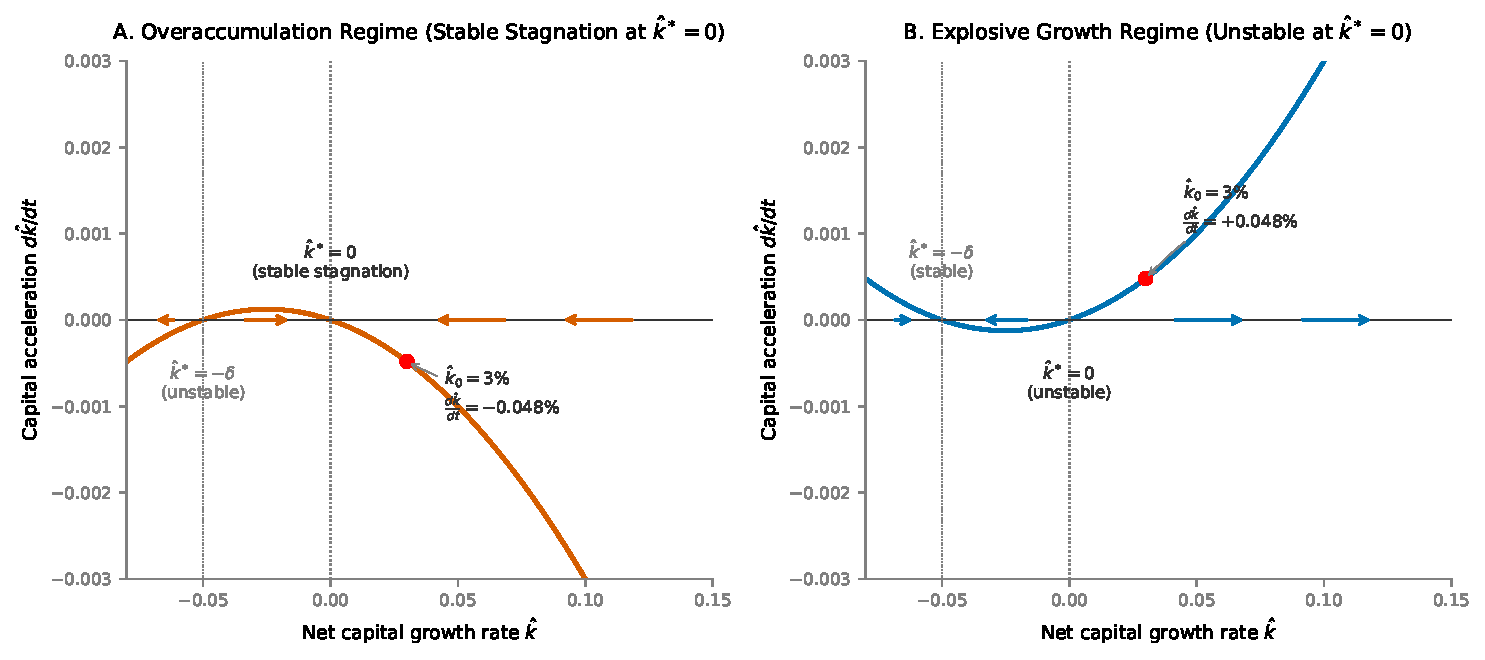
\includegraphics[width=0.92\linewidth]{figures/fig_S3_phase_diagram_capital_capacity_dynamics.pdf}
\caption*{\footnotesize Note: Panel A plots the overaccumulation regime ($\theta = 0.8 < 1.0$) where capital acceleration is negative for $\hat{k} > 0$ ($d\hat{k}/dt < 0$), pushing the net accumulation rate toward the stable stagnation equilibrium at $\hat{k}^* = 0$ (while $\hat{k}^* = -\delta$ represents the unstable lower boundary). Panel B plots the explosive growth regime ($\theta = 1.2 > 1.0$) where capital acceleration is positive for $\hat{k} > 0$ ($d\hat{k}/dt > 0$), causing the accumulation rate to diverge from $\hat{k}^* = 0$. Both panels show the initial condition $\hat{k}_0 = 3\%$ where $d\hat{k}/dt = \mp 0.048\%$, consistent with the numerical example in \S\ref{subsec:balanced_unbalanced_growth}.}
\label{fig:ode_phase_diagram}
\end{figure}

\subsection{Trend Stabilization, Viability Condition, and the Double-Misspecification Bias}
\label{subsec:trend_stabilized_closure}

Introducing a deterministic time trend ($b$) into the unbalanced growth closure ($g_{Y^p} = \theta g_K + b$) alters the dynamic properties of the system. Substituting this closure into the acceleration equation produces a quadratic differential equation:
\begin{equation}
\frac{d\hat{k}}{dt} = (\hat{k} + \delta)\left[(\theta - 1)\hat{k} + b\right].
\end{equation}
Under overaccumulation ($\theta < 1$) with positive technical progress ($b > 0$), this specification creates a locally stable interior steady state:
\begin{equation}
\hat{k}^* = \frac{b}{1 - \theta}.
\end{equation}
The ratio $b / (1 - \theta)$ balances autonomous technical progress against the drag of overaccumulation, preventing the net accumulation rate from falling to zero (as detailed in Appendix~\ref{app:acc_dynamics}).

However, treating this trend-stabilized path as an exogenous technical baseline is conceptually problematic. Following \citet{Basu2022}, technical change under capitalism is constrained by capitalist viability: profit-seeking firms adopt new techniques only if they reduce unit production costs at prevailing wages and input prices. The direction of technical change---whether capital-using and labor-saving or capital-saving and labor-saving---is endogenously shaped by class conflict over the real wage relative to labor productivity. Consequently, a deterministic time trend ($bt$) in the capacity regression does not capture neutral technical progress; it acts as an econometric sponge that absorbs the cumulative effects of distributional conflict and induced technical change.

This setup creates a risk of compound misspecification in econometric estimation. As \citet{Basu2020} emphasizes, when an empirical model omits a relevant variable---such as distribution influencing the choice of technique \citep{Kurz1986}---while including an exogenous proxy such as a deterministic trend, the estimated coefficient on capital suffers from compound bias. The trend mathematically absorbs unobserved shifts in distribution, compromising the structural interpretation of the recovered elasticity $\theta$.

Furthermore, estimating this relation over a 64-year sample (1947--2011) assumes that $\theta$ and $b$ remain invariant across major structural shifts: the post-war boom (1947--1973), the stagflation transition (1974--1982), and the neoliberal era (1983--2011). Imposing fixed coefficients forces the model to average across distinct institutional and macroeconomic regimes.

Finally, this framework connects to theoretical debates on the endogeneity of investment. In Neo-Kaleckian models, capital accumulation adjusts endogenously to demand-induced utilization gaps, whereas Sraffian supermultiplier models treat investment as anchored in autonomous demand components and cost-minimizing technique choices. Examining whether capital accumulation responds to long-run capacity disequilibria provides an empirical test of these alternative adjustment mechanisms. The subsequent empirical sections implement this replication and testing strategy.

\section{Critical Replication Study on Shaikh’s Approach to Cointegration}
\label{sec:replication_strategy}
\subsection{Econometric Framework and Staged Design}
\label{subsec:econometric_framework_design}

Shaikh’s long-run output–capital coefficient does not identify a stable, time-invariant capacity benchmark; it mechanically averages over historically distinct distributive regimes. As established in Section 3, this coefficient functions as a transformation elasticity ($\theta$) linking capital accumulation to capacity formation under conditions of unbalanced growth. This section tests whether a single, full-sample estimation can capture this relationship, or whether the bivariate relation is fundamentally misspecified without explicit distributional conditioning. By testing the cointegrating relation directly rather than relying on a pre-fabricated utilization index, I subject the underlying classical capacity theory to empirical testing.

I execute this critical investigation across three sequential stages of increasing econometric generality. In Stage S0, I reconstruct the closest empirical counterpart to Shaikh's baseline single-equation model to verify its basic numerical reproducibility. Stage S1 lifts the baseline's rigid specification choices by estimating a combinatoric grid of 500 Autoregressive Distributed Lag (ARDL) models, mapping how the estimated transformation elasticity ($\hat{\theta}$) shifts under alternative lag structures, trend configurations, and outlier controls. Finally, Stage S2 transitions the analysis from single-equation models to system-level estimations, testing whether the output--capital relation survives as a stable Vector Error Correction Model (VECM) and checking whether it requires the rate of exploitation ($e_t$) to establish system-level cointegration.

The results show that while Shaikh's baseline coefficient is numerically reproducible, it is neither structurally unique nor stable in isolation. In the single-equation grid search, the estimated elasticity ranges from 0.65 to 0.92 depending on how model complexity is penalized, indicating that the baseline point estimate is highly sensitive to researcher choices. More importantly, the standalone output--capital relation fails system-level cointegration tests, showing that a stable long-run relationship cannot be identified in a full-sample bivariate setting. The output--capital relation achieves system stability only within a trivariate framework that includes the rate of exploitation, showing that the long-run conversion of capital to capacity is structurally conditioned by the historical distribution of income between wages and profits.

I present these results sequentially across seven subsections. First, Subsection~\ref{subsec:econometric_framework_design} outlines the mathematical framework and staged design. Subsection~\ref{subsec:data_measurement} details the data construction, measurement conventions, and stylized facts. Subsection~\ref{subsec:admissibility_strategy} defines the admissibility filters and diagnostic screens. Subsections~\ref{subsec:S0_reproducibility_new}, \ref{subsec:S1_admissible_spec_new}, and \ref{subsec:S2_vecm} present the empirical results for Stages S0, S1, and S2, respectively. Finally, Subsection~\ref{subsec:cross_stage_synthesis_design_new} provides a cross-stage econometric synthesis.

Table~\ref{tab:cross_stage_synthesis_design} formalizes this progressive testing sequence, outlining the design object, specification space, and diagnostic criteria for each stage. Moving from a single-point reconstruction (S0) to a combinatorial specification grid (S1) systematically maps how parameter estimates respond to model complexity. The transition to joint system estimation (S2) then tests whether these single-equation relationships survive as self-sufficient economic attractors once bidirectional feedbacks are permitted. This staged architecture separates the statistical fit of the model from the historical and institutional validity of its derived capacity path.

\begin{table}[h!]
\centering
\scriptsize
\caption{Stage Design and Admissibility Strategy}
\label{tab:cross_stage_synthesis_design}
\begin{tabular}{@{}>{\raggedright\arraybackslash}p{1.6cm}>{\raggedright\arraybackslash}p{2.6cm}>{\raggedright\arraybackslash}p{3.0cm}>{\raggedright\arraybackslash}p{3.2cm}>{\raggedright\arraybackslash}p{3.2cm}@{}}
\toprule
Stage & Design Object & Specification Space & Admissibility and Organization & Interpretive Implication \\
\midrule
\midrule
S0 & Single-point reconstruction of baseline specification & ARDL(2,4), historical step controls ($S_{yy,t}$), alternative deterministic closures & F-bounds primary screen; t-bounds diagnostic where defined; utilization path proximity & Tests whether a deterministic capacity path can be closely reconstructed \\
S1 & ARDL specification grid $\mathcal{G}_{S1}$ & Lag orders $(p,q)$, five PSS cases, four nested dummy structures & F-admissible set $\mathcal{A}^{F}_{S1}$; F+t confirmed candidates $\mathcal{C}_{S1}$; corrected envelope $E_{S1}$; IC-specific neighborhoods $\mathcal{F}^{(0.20)}_j$ & Tests whether the output--capital coefficient is structurally unique or varies with IC penalty logic \\
S2 Bivariate & Joint $(\ln Y_t, \ln K_t)'$ VECM & Lag order, deterministic branch, dummy structure, $r=1$ & Triple gate $\mathcal{A}_{S2}$: convergence, Johansen rank, companion stability & Tests whether the bilateral output--capital relation is self-sufficient at the system level \\
S2 Trivariate & Joint $(\ln Y_t, \ln K_t, \ln e_t)'$ VECM & Same as bivariate, with logged rate of exploitation included; $r=1$ or $r=2$ & Same triple gate; $\Omega_{20}$ organizes admissible survivors by log-likelihood loss & Tests whether the structural relation survives exclusively when distribution enters explicitly \\
\bottomrule
\end{tabular}
\caption*{\footnotesize Note: This table outlines the progressive multi-stage replication architecture. The sequence advances from baseline single-equation reconstruction (S0) through parameter sensitivity grids (S1) to joint system-level survival testing (S2). Source: Author's elaboration.}
\end{table}

To evaluate whether output ($y_t$) and capital ($k_t$) share a stable long-run equilibrium, I specify the output--capital relation as an Autoregressive Distributed Lag (ARDL) model and apply the bounds-testing procedure developed by \citet{Pesaran2001}. Cointegration means that although output and capital drift over time as nonstationary series, they are tied together by a long-run equilibrium relationship that prevents them from drifting apart indefinitely. This framework detects cointegration regardless of whether the individual series are integrated of order zero ($I(0)$) or one ($I(1)$), avoiding fragile unit-root pre-testing.

This relationship is estimated using an unrestricted error correction model (UECM) derived from a general $\text{ARDL}(p, q)$ specification:
\begin{equation}
\Delta y_t = c_0 + c_1 t + \pi_y y_{t-1} + \pi_k k_{t-1} + \sum_{i=1}^{p-1} \psi_{y,i} \Delta y_{t-i} + \sum_{j=0}^{q-1} \psi_{k,j} \Delta k_{t-j} + \sum_{h=1}^{H} \delta_h S_{h,t} + \varepsilon_t .
\label{eq:ardl_uecm}
\end{equation}

This unrestricted error-correction representation separates short-run adjustment dynamics from the long-run level relationship. In equation~\eqref{eq:ardl_uecm}, $c_0$ is the intercept, $c_1 t$ is a deterministic linear time trend, and $\varepsilon_t$ is an independent and identically distributed error term. The differenced terms $\Delta y_{t-i}$ and $\Delta k_{t-j}$ capture short-run dynamics, where $p$ and $q$ represent the lag lengths of output and capital. The lagged level terms $y_{t-1}$ and $k_{t-1}$ contain the long-run cointegrating relationship. The historical step indicators $S_{h,t} \equiv \mathbf{1}\{t \ge h\}$ absorb permanent regime shifts (such as the 1974 oil shock and post-1980 restructuring), preventing structural breaks from distorting the underlying long-run relationship.

The statistical distribution of the bounds test depends on the restrictions placed on the constant and linear trend in the model. \citet{Pesaran2001} outline five deterministic configurations (Cases I through V) that determine how the constant $c_0$ and time trend $t$ enter the equation. These cases range from Case I (no constant, no trend) to Case V (unrestricted constant and unrestricted trend), including intermediate cases where constants or trends are restricted to the long-run cointegrating space. Since these deterministic components alter the asymptotic behavior of the nonstationary variables, each case requires a different set of critical value bounds. These five configurations represent specification choices that alter the statistical boundaries of the cointegration test.

A joint Wald $F$-bounds test evaluates the null hypothesis that no long-run relationship exists between output and capital. The null hypothesis ($H_0^F$) asserts that the coefficients on the lagged level terms are jointly zero, meaning there is no cointegration:
\begin{equation}
H_{0}^{F}: \pi_y=\pi_k=0, \qquad H_{a}^{F}: (\pi_y,\pi_k)\neq(0,0).
\label{eq:fbounds_hypothesis}
\end{equation}

Under this hypothesis, $\pi_y$ and $\pi_k$ are the coefficients on the lagged levels of output and capital. If the null is true, the regression is spurious because the residuals remain nonstationary ($I(1)$), rendering any derived capacity path econometrically invalid. To evaluate the Wald statistic, I use the critical bounds generated by \citet{Pesaran2001}. These bounds establish two thresholds: a lower bound assuming all variables are $I(0)$, and an upper bound assuming all variables are $I(1)$. The null of no cointegration is rejected only when the computed $F$-statistic exceeds the upper bound, confirming that the output--capital relation yields stationary residuals.

The $t$-bounds test serves as a secondary confirmation screen to ensure that the cointegrating relationship is stable. The Wald $F$-test can find pseudo-cointegration if only one of the lagged level variables is significant. The $t$-bounds test evaluates the null hypothesis that the coefficient on the lagged dependent variable ($\pi_y$) is zero:
\begin{equation}
H_{0}^{t}: \pi_y=0, \qquad H_{a}^{t}: \pi_y<0.
\label{eq:tbounds_hypothesis}
\end{equation}

This is tested against the one-sided alternative hypothesis ($\pi_y < 0$), which requires the error-correction coefficient to be negative. A negative speed-of-adjustment coefficient acts as a restoring force: when actual output drifts away from its long-run capacity path, the system adjusts by pulling output back toward equilibrium. If $\pi_y$ is positive or zero, the system is explosive or has no restoring mechanism. Given the relatively short sample period ($T \approx 65$), I use finite-sample critical bounds from \citet{NatsiopoulosTzeremes2022} rather than asymptotic tables to prevent over-stating cointegration significance.

To recover the long-run transformation elasticity ($\theta$), one must distinguish the underlying levels ARDL model from its error-correction representation. The general levels $\text{ARDL}(p, q)$ specification is:
\begin{equation}
y_t = a_0 + a_1 t + \sum_{i=1}^p \alpha_i y_{t-i} + \sum_{j=0}^q \beta_j k_{t-j} + \sum_{h=1}^H \delta_h S_{h,t} + \varepsilon_t .
\label{eq:ardl_levels}
\end{equation}
From this levels model, the long-run multiplier ($d$) is recovered as the sum of the capital stock coefficients normalized by the output lag coefficients:
\begin{equation}
\hat{d} = \frac{\sum_{j=0}^q \hat{\beta}_j}{1 - \sum_{i=1}^p \hat{\alpha}_i} .
\label{eq:d_levels}
\end{equation}
This levels ratio represents the steady-state multiplier where dynamic adjustment processes have fully settled. In his baseline estimation, Shaikh treats this parameter as a constant technical coefficient mapping capital directly to potential capacity. Under the conceptual framework developed here, however, I interpret this long-run coefficient as a capacity transformation elasticity, $\theta$, which is historically and distributionally conditioned.\footnote{Shaikh's original exposition \citep{Shaikh2016} seldom discusses the parameter $d$ as an elasticity, treating it instead as a fixed accounting coefficient. I interpret this long-run multiplier $d$ as the empirical proxy for the capacity transformation elasticity $\theta$ under conditions of unbalanced growth. For clarity, I retain the notation $d$ when replicating Shaikh's ARDL specifications directly, and transition to $\theta$ when developing the conceptual and system VECM extensions.}

This levels specification maps directly to the unrestricted error correction model (UECM) in Equation~\eqref{eq:ardl_uecm} by reparameterizing the level variables around their first-difference representations. In the UECM, the speed-of-adjustment coefficient $\pi_y$ and the level capital coefficient $\pi_k$ relate to the levels parameters by $\pi_y = -(1 - \sum_{i=1}^p \alpha_i)$ and $\pi_k = \sum_{j=0}^q \beta_j$. Thus, the long-run multiplier is recovered from the conditional UECM parameters as the ratio:
\begin{equation}
\hat{d} = -\frac{\pi_k}{\pi_y} .
\label{eq:d_recovery}
\end{equation}
This UECM ratio is mathematically identical to the levels ratio in Equation~\eqref{eq:d_levels}. Only the levels coefficients enter the long-run relation to ensure that the parameter reflects the steady-state level relationship.

In Shaikh's procedure, this long-run multiplier anchors the fitted capacity path. Capacity utilization is then the residual deviation from the long-run cointegration vector: $\log \hat{\mu}_t = y_t - \hat{y}^p_t$. This design makes utilization dependent on the estimated coefficient. Shaikh treats the coefficient as a fitted accounting multiplier, but leaves its structural role unanalyzed. I re-interpret the coefficient as a transformation elasticity $\hat{\theta}$ of productive capacities with respect to capital accumulation, subject to the specification grid, deterministic treatment, and admissibility gates. I evaluate this elasticity across three stages: reconstructing the baseline result (Stage S0), evaluating the single-equation specification space (Stage S1), and testing whether the relation survives in a joint system (Stage S2). Subsection~\ref{subsec:data_measurement} details the data construction and measurement conventions required to execute these steps.

Stage S0 tests the reproducibility of Shaikh's baseline results to establish a benchmark for replication. I target his published single-equation model, fix the lag structure at the reported ARDL(2,4) configuration, and estimate the parameters using the closest recoverable corporate-sector data identified from his published tables. I estimate these baseline parameters across alternative deterministic configurations and historical step controls to evaluate numerical reproducibility.

This procedure estimates the long-run relationship, constructs the potential capacity path, and calculates capacity utilization as the residual deviation of actual output from that path. Cointegration bounds tests distinguish long-run level relations from spurious correlations. Within the ARDL framework, while the $F$-bounds test applies to all five deterministic cases, the $t$-bounds test is defined only for Cases I, III, and V; specifications under Case II or Case IV cannot be screened using the $t$-bounds gate.

\subsubsection{Stage 1 \texorpdfstring{$(S1)$}{}: Admissible-Specification Stress Test}
\label{subsec:S1_admissible_spec}

In Stage S1, I expand the single-equation model into a combinatoric grid of 500 different specifications. By varying lag lengths, deterministic trends, and outlier controls, I evaluate how modeling choices affect cointegration outcomes and the estimated elasticity. This approach shifts focus from a single preferred model to the entire space of specifications, showing how sensitive the capacity path is to modeling choices.

Output and capital lags vary freely from 1 to 5 ($p, q \in \{1, \dots, 5\}$). Each lag combination is estimated across all five deterministic cases, combined with four alternative blocks of historical dummy variables ($s_0$ through $s_3$). These dummies control for major post-war disruptions: the 1956 post-Korean defense cuts, the 1974 oil price shock, and the 1980 Volcker monetary contraction. Permuting these options yields 500 unique models. Formally, the specification space is:
\begin{equation}
\mathcal{G}_{S1} = \{(p,q,c,s)\},
\label{eq:G_S1}
\end{equation}
where each element $(p, q, c, s)$ represents a single model with lag orders $p$ and $q$, PSS case configuration $c$, and outlier control block $s$.

Admissibility screens filter out models that fail cointegration tests, but do not isolate a unique parameter. To organize the cointegrating models, I construct a fit-complexity envelope ($E_{S1}$) that identifies the optimal trade-off between statistical fit and parameter count:
\begin{equation}
E_{S1} = \{ m \in \mathcal{A}^{F}_{S1} : \nexists m' \in \mathcal{A}^{F}_{S1} \text{ with } L(m') \leq L(m) \text{ and } K(m') \leq K(m) \},
\label{eq:E_S1}
\end{equation}
where $L(m) = -2\log\hat{\ell}(m)$ is model deviance and $K(m)$ is parameter count. A model lies on $E_{S1}$ only if no other cointegrating model fits better while using fewer parameters.

Information-criterion neighborhoods ($\mathcal{F}^{(0.20)}_j$) capture competitive specifications near the Pareto frontier:
\begin{equation}
\mathcal{F}^{(0.20)}_j = \{ m \in \mathcal{A}^{F}_{S1} : IC_j(m) \leq Q_{0.20}(IC_j \mid \mathcal{A}^{F}_{S1}) \},
\label{eq:F_j}
\end{equation}
where $j$ indexes the Akaike Information Criterion (AIC), Bayesian Information Criterion (BIC), Hannan-Quinn (HQ), and Bozdogan's Information Complexity Index (ICOMP) along with its robust variant (RICOMP). While AIC and BIC penalize parameter counts, ICOMP and RICOMP penalize parameter interdependence and covariance complexity. This variety illustrates how different penalty structures select different elasticity estimates across the specification space.

Each specification $m$ yields an estimate of the transformation elasticity $\hat{\theta}(m)$, determining the slope of the capacity path:
\begin{equation}
\hat{\mu}_t(m) = y_t - [\hat{a}(m) + \hat{b}(m)t + \hat{\theta}(m)k_t].
\label{eq:mu_hat_m}
\end{equation}

Table~\ref{tab:s1_stress_synthesis} summarizes the structure of this single-equation specification search. The empirical results of this grid search are reported in Subsection~\ref{subsec:S1_admissible_spec_new}.

\begin{table}[h!]
\centering
\small
\caption{Synthesis of Admissibility Specification Stress Tests}
\label{tab:s1_stress_synthesis}
\begin{tabular}{@{}>{\raggedright\arraybackslash}p{3.2cm}>{\raggedright\arraybackslash}p{2.6cm}>{\raggedright\arraybackslash}p{3.8cm}>{\raggedright\arraybackslash}p{4.0cm}@{}}
\toprule
\toprule
Stress-Test Component & Operational Layer & Screening/Organization Rule & Diagnostic Target \\
\midrule
\midrule
Cointegration admissibility & F/T-bounds sequence & $p_F(m) \leq \alpha$, $p_t(m) \leq \alpha$ (if defined) for $\alpha \in \{0.10, 0.05, 0.01\}$ & Existence and significance of long-run level relationships \\
Specification invariance & Lag-order variation & Monitor parameter drift $\hat{\theta}(m)$ across combinatoric $p,q \in \{1,\dots,5\}$ & Stability and unique mapping of the long-run structural multiplier \\
Identification fragility & Deterministic cases \& dummy structures & Track admissibility shifts across $c \in \{1,\dots,5\}$ and $s \in \{s_0,\dots,s_3\}$ & Sensitivity to deterministic components and structural trend assumptions \\
Information complexity \& Pareto optimization & Fit-complexity envelope \& IC neighborhoods & Pareto non-dominance in $E_{S1}$; 20th percentile cutoff for $j \in \{\text{AIC}, \text{BIC}, \text{HQ}, \text{ICOMP}, \text{RICOMP}\}$ & Organization of disciplined non-uniqueness under distinct information penalty schedules \\
Capacity benchmark sensitivity & Utilization path fan $\hat{\mu}_t(m)$ & Map structural parameter variance to latent residual series & Macroeconomic consequence of single-equation coefficient drift on normal profit estimation \\
\bottomrule
\end{tabular}
\caption*{\footnotesize Note: This synthesis matrix outlines the nested single-equation admissibility screens, information-theoretic optimization layers, and diagnostic targets within the stage $S1$ multi-model grid. Source: Author's elaboration.}
\end{table}

Stage S2 extends this analysis to a joint multi-equation system, testing whether bivariate cointegration holds when output and capital are both treated as endogenous, and whether establishing a stable long-run relationship requires including the rate of exploitation ($e_t$).

\subsubsection{Stage 2 \texorpdfstring{$(S2)$}{}: System Cointegration Test}
\label{subsec:S2_system}

Stage S2 tests whether the output--capital relation remains stable in a multi-equation system. If output and capital are cointegrated, a bivariate vector $X_t = (\ln Y_t, \ln K_t)'$ should exhibit a stable cointegrating relationship under Johansen's rank tests. However, as shown below, this bivariate system fails to cointegrate over the full post-war sample. I evaluate whether introducing the logged rate of exploitation, $e_t = \ln(\pi_t / (1 - \pi_t))$, to form the trivariate vector $X_t = (\ln Y_t, \ln K_t, \ln e_t)'$ establishes a stable cointegrating relationship. This trivariate system is estimated using a Vector Error Correction Model (VECM):
\begin{equation}
\label{eq:vecm_johansen}
\Delta X_t = \Pi X_{t-1} + \sum_{i=1}^{p-1} \Gamma_i \Delta X_{t-i} + \Phi D_t + \varepsilon_t,
\end{equation}
where $\Gamma_i$ represents short-run dynamics, $D_t$ contains deterministic components and dummies, and $\Pi = \alpha \beta'$ is the long-run impact matrix. A stable cointegrating relation exists when $\Pi$ has reduced rank $r=1$, with the exploitation variable entering the cointegrating space $\beta$.

The stability of this system is evaluated across a grid of VECM specifications, varying lag structures, trend configurations, and outlier dummies. For each target rank $r$, the attempted specification space is:
\begin{equation}
\mathcal{G}_{S2}^{(r)} = \{(p, C_{\text{det}}, s)\},
\label{eq:G_S2}
\end{equation}
where $p$ represents the VAR lag orders (from 1 to 4), $C_{\text{det}}$ indexes the four deterministic configurations, and $s$ selects the outlier step controls ($C_0$: no constant/trend; $C_1$: restricted constant in cointegrating space; $C_2$: unrestricted short-run constant; $C_3$: unrestricted constant and trend). Permuting these choices yields 48 attempted models. Restricted constant models ($C_1$) are excluded because they systematically fail numerical convergence in \texttt{tsDyn}, leaving 36 estimated models in the grid.

\subsection{Data, Measurement, and Stylized Facts}
\label{subsec:data_measurement}

I use annual US corporate sector data from 1947 to 2011 ($T = 65$), sourced from the data companion in \citet{Shaikh2016}.\footnote{Replication data and construction scripts are available at: \url{https://www.realecon.org/data}. While Shaikh specifies a common-deflator condition, he does not name the price index; a GPIM-consistent price deflator is implemented here to ensure reproducibility.} Capacity utilization is the residual deviation of actual output from the cointegrated output--capital path. Table~\ref{tab:variables_replication} summarizes the variables, their construction, and measurement conventions.

\begin{table}[h!]
\centering
\caption{Core replication variables: symbols, sources, and transformations}
\label{tab:variables_replication}
\small
\begin{tabular}{@{}>{\raggedright\arraybackslash}p{2.8cm}>{\raggedright\arraybackslash}p{4.5cm}>{\raggedright\arraybackslash}p{2.2cm}>{\raggedright\arraybackslash}p{3.2cm}@{}}
\toprule
Symbol & Construction & Role & Measurement constraint \\
\midrule
$\text{GVAcorp}_t$ & NIPA Table 1.14 (L1) + imputed-interest adj. (Table 7.11) & Output flow & Classical surplus correction \\
$\text{KGCcorp}_t$ & BEA Fixed Asset 6.1 (L9) + IRS SOI + GPIM recursion & Capital anchor & GPIM stock--flow reconstruction \\
$p_t$ & $pKN$ implicit price deflator, 2005=100 & Common price basis & GPIM-consistent deflation \\
$y_t$ & $\ln(\text{VAcorp}_t/p_t)$ & Dependent variable & Inherits output and deflator choices \\
$k_t$ & $\ln(\text{KGCcorp}_t/p_t)$ & Regressor & Inherits GPIM depletion rates \\
$S_{56},S_{74},S_{80}$ & Step estimation controls ($\mathbf{1}\{t \ge yy\}$) & Regime-shift absorbers & Baseline structural break absorption \\
\bottomrule
\end{tabular}
\caption*{\footnotesize Note: Stage $S2$ introduces $\ln e_t$ (logged exploitation) to the trivariate state vector. Distributional variables enter at the multi-equation system stage. Full series definitions, sources, and transformations are provided in Table~\ref{tab:app_glossary} of Appendix~\ref{app:data_construction}.}
\end{table}

To reconstruct the gross capital stock, I use the Generalized Perpetual Inventory Method (GPIM) following \citet{Shaikh2016}. This accounting framework calculates capital stock from nominal gross investment flows, annual depreciation rates, and an implicit deflator built from gross capital formation accounts. The recursion accumulates current-cost capital as:
\begin{equation}
K_t = IG_t + z_t^* \cdot K_{t-1},
\qquad
z_t^* \equiv (1 - z_t) \frac{p^K_t}{p^K_{t-1}},
\end{equation}
where $IG_t$ is nominal gross investment, $z_t$ is the annual depreciation rate, and $z_t^*$ reflates surviving capital to current replacement cost. I follow Shaikh's three adjustments to construct this series: replacing the BEA 2011 infinite-lives assumption with BEA 1993 service lives, anchoring initial values to 1925 benchmarks, and rescaling the historical stock over 1925--1947 using the IRS corporate book-value index \citep[Appendix~6.7]{Shaikh2016}. The constructed series closely tracks the BEA official net stock with a 99.60\% average ratio over 1947--2005, confirming that differences in levels reflect these methodological choices. Appendix~\ref{subsec:app_gpim} contains the full recursion inputs and depreciation rates.

Both output and capital are deflated by the $pKN$ price index (2005=100) to maintain stock-flow consistency. Standard BEA releases use quality-adjusted chain weights that alter the measured volume of investment across generations of capital, which is inconsistent with the physical stock-flow construction used here. Deflating by the $pKN$ index follows Shaikh's convention, ensuring that the output--capital relation reflects productive equipment rather than quality adjustments \citep[Appendix~6.6]{Shaikh2016}.

Corporate gross value added is adjusted for imputed financial intermediation services (FISIM) following NIPA Table 7.11 (Appendix~\ref{subsec:app_impint}). Step-shift controls ($S_{1956,t}$, $S_{1974,t}$, $S_{1980,t}$, where $S_{yy,t} \equiv \mathbf{1}\{t \ge yy\}$) are included in the estimation regressions to absorb permanent institutional and macroeconomic disruptions: the 1956 post-Korean defense cuts, the 1974 OPEC oil crisis, and the 1980 Volcker monetary contraction (see Appendix~\ref{app:data_construction} for pulse diagnostic indicators $P_{yy,t}$). Given the sample size ($T = 65$), finite-sample bounds are computed using stochastic simulations \citep{NatsiopoulosTzeremes2022}. Regarding time-series properties, Pesaran--Shin--Smith bounds inference accommodates regressors that are $I(0)$ or $I(1)$, but not $I(2)$. Complementary unit-root and stationarity diagnostics (Appendix~\ref{subsec:app_desc_stats}) support treating $k_t$ as $I(1)$, removing the specific concern that capital stock may fall outside the admissible $I(0)/I(1)$ range, while providing an integration-order treatment consistent with the maintained assumptions of the system-level VECM.

These measurement choices are central to the empirical strategy. I use Shaikh's GPIM-adjusted gross capital stock because the objective is to measure physical equipment in operation rather than asset valuations. While net capital stock measures are appropriate for evaluating profit rates and wealth, gross capital stock serves as the preferred anchor for the capacity concept used here. Using gross capital stock reduces distortions from accounting depreciation rules and asset revaluations, which make net capital stock growth rates more volatile than physical capacity. Appendix~\ref{subsec:app_gpim} details the specific recursion parameters.

Between 1947 and 2011, post-war US capital accumulation outpaced output and employment growth, driving a secular decline in the output--capital ratio that mirrors the broader OECD experience of Marx-biased technical change. Specifically, the real corporate gross capital stock grew at an average annual rate of 4.1\%, while real output expanded at 3.0\% and employment grew at 1.3\%. Cross-country evidence confirms that labor productivity across advanced capitalist economies rises primarily through mechanization and capital-using, labor-saving technical change \citep{Marquetti2003, Basu2010}. This persistent downward drift in the output--capital ratio motivates empirical testing of whether a fixed technical coefficient can adequately describe the post-war record, or whether the conversion of capital into productive capacity is conditioned by distributive conflict and choice of technique.

Figures \ref{fig:main_log_levels}, \ref{fig:main_output_capital_ratio}, and \ref{fig:main_growth_rates} plot these post-war trends. While output and capital grow together over the long run (Figure \ref{fig:main_log_levels}), their ratio is subject to long historical swings rather than remaining constant (Figure \ref{fig:main_output_capital_ratio}). As shown in Figure \ref{fig:main_growth_rates}, output growth exhibits higher volatility than capital accumulation. The lower volatility of gross capital stock reflects its insulation from valuation shocks, tracking physical equipment in use.

\begin{figure}[H]
\centering
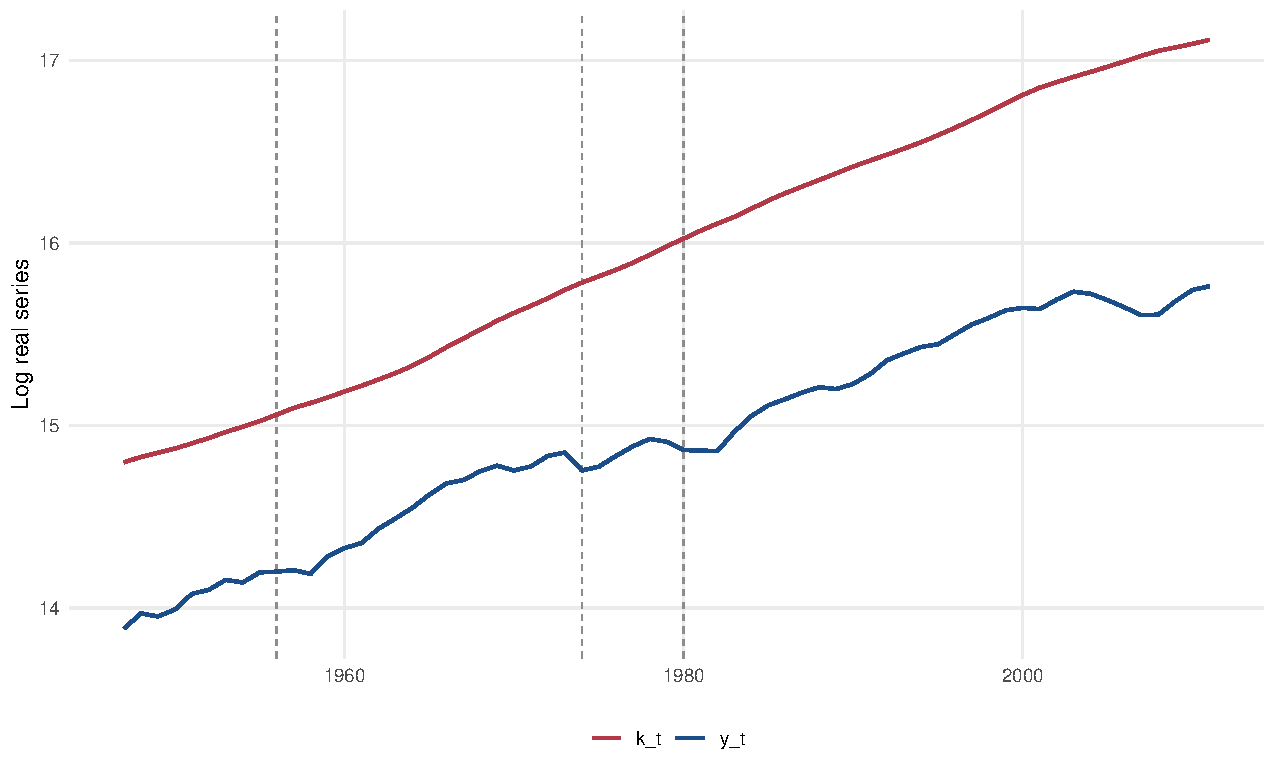
\includegraphics[width=0.85\textwidth]{appendixA/figures/fig_A1_log_output_capital.pdf}
\caption{Log output ($y_t$) and log capital ($k_t$), 1947--2011. Vertical dashed lines mark 1956, 1974, and 1980.}
\label{fig:main_log_levels}
\end{figure}

\begin{figure}[H]
\centering
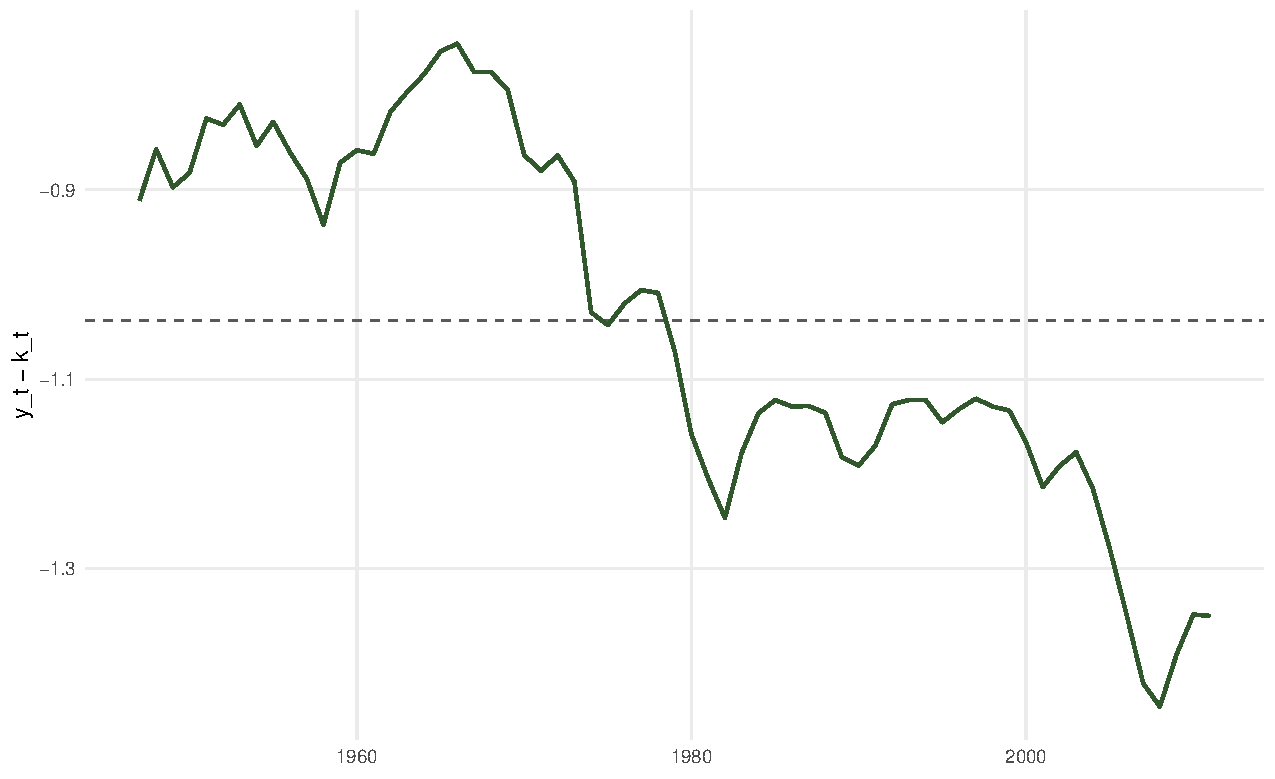
\includegraphics[width=0.85\textwidth]{appendixA/figures/fig_A2_output_capital_ratio.pdf}
\caption{Output--capital ratio ($y_t - k_t$), 1947--2011. Horizontal line marks long-run mean.}
\label{fig:main_output_capital_ratio}
\end{figure}

\begin{figure}[H]
\centering
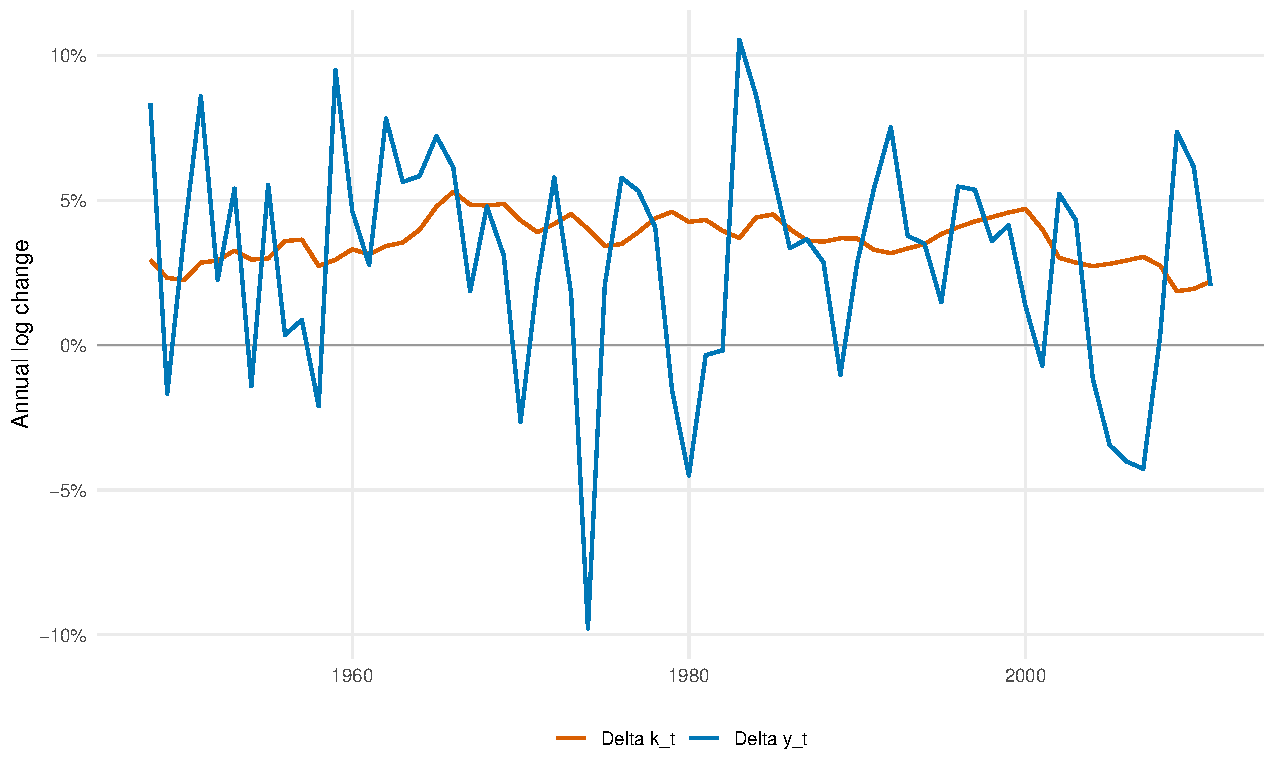
\includegraphics[width=0.85\textwidth]{appendixA/figures/fig_A3_growth_rates.pdf}
\caption{Annual growth rates of output ($\Delta y_t$), gross capital ($\Delta k_t$), and net capital ($\Delta k^{net}_t$), 1947--2011.}
\label{fig:main_growth_rates}
\end{figure}

\subsection{The Admissibility Strategy}
\label{subsec:admissibility_strategy}

In this paper, an admissible specification is one that produces stationary residuals and stable dynamic roots. If an estimated model fails cointegration, its residuals contain a unit root, meaning output and capital drift apart without a long-run equilibrium. Capacity utilization series derived from non-cointegrated specifications are spurious, as the estimated capacity ceiling wanders away from actual output.

For single-equation ARDL models (Stages~S0 and~S1), admissibility requires the specification to pass the \citet{Pesaran2001} bounds test: the Wald $F$-statistic must exceed the upper critical bound at the 5\% level. For multi-equation models (Stage~S2), admissibility requires three conditions: convergence of the maximum likelihood estimation, rejection of the zero-rank null hypothesis in the Johansen trace test at the 5\% level ($r=1$), and dynamic stability of the companion matrix (all eigenvalues strictly within the unit circle). Specifications failing any of these conditions are excluded from model comparison. Formally, the single-equation $F$-admissible set $\mathcal{A}^{F}_{S1}$ is defined as:
\begin{equation}
\mathcal{A}^{F}_{S1} = \{ m \in \mathcal{G}_{S1} : p_F(m) \leq 0.10 \},
\label{eq:A_F_S1}
\end{equation}
where $p_F(m)$ is the $p$-value of the Wald bounds test for model $m$. If this probability is 10\% or less, the specification enters the admissible pool. Models that yield a Wald statistic below the lower critical bound or within the inconclusive interior band are discarded.

The secondary screen uses the $t$-bounds test to verify error-correction stability. Because the $t$-bounds statistic is only defined for deterministic Cases I, III, and V, specifications using Cases II and IV bypass this test. The $t$-admissible set $\mathcal{T}_{S1}$ is:
\begin{equation}
\mathcal{T}_{S1} = \{ m \in \mathcal{A}^{F}_{S1} : p_t(m) \leq 0.10 \text{ if defined} \},
\label{eq:T_S1}
\end{equation}
where $p_t(m)$ is the $p$-value for the one-sided $t$-test on the error-correction coefficient $\pi_y$. A significant negative coefficient confirms that output adjusts back toward the long-run capacity ceiling after a shock. To identify specifications that pass both the Wald and error-correction tests at the stricter 5\% level, the Strong Cointegration Space $\mathcal{C}_{S1}$ is defined as:
\begin{equation}
\mathcal{C}_{S1} = \{ m \in \mathcal{T}_{S1} : p_F(m) \leq 0.05 \text{ and } p_t(m) \leq 0.05 \}.
\label{eq:C_S1}
\end{equation}

In a ``no-dummy'' counterfactual specification omitting the historical step controls ($S_{1956,t}$, $S_{1974,t}$, $S_{1980,t}$), residuals remain nonstationary ($I(1)$) across all lag profiles in the tested grid, failing the cointegration bounds tests. This counterfactual indicates that controlling for major historical disruptions is necessary to achieve cointegrating residuals in the bivariate setting.

In Stage S2, the specification space is filtered through a mechanical triple-admission gate to ensure that surviving models constitute stable multi-equation attractors rather than spurious or explosive regressions. First, the Estimation Convergence Gate requires the numerical maximum likelihood estimation to converge cleanly without boundary pathologies. Second, the Cointegration Rank Gate requires the Johansen trace test to reject the null hypothesis of zero cointegrating vectors ($r=0$) at the 5\% level while failing to reject at most one cointegrating vector ($r \leq 1$). Third, the Dynamic Stability Gate requires all non-zero eigenvalues of the VECM companion matrix to lie strictly inside the unit circle (excluding the $m - r$ unit roots associated with common stochastic trends), eliminating explosive systems. Mechanically surviving models are subsequently evaluated through diagnostic quality screens (multivariate normality, ARCH effects, and serial correlation) to assess residual properties without treating these diagnostics as mechanical rejection criteria. Surviving VECMs are then organized by information criteria and log-likelihood values to identify focal empirical attractors.

\subsection{Stage 0 \texorpdfstring{$(S0)$}{}: Single-Equation Reconstruction}
\label{subsec:S0_reproducibility_new}

Stage S0 evaluates whether Shaikh's baseline capacity path is numerically reproducible. Reconstructing this benchmark requires tracing data vintages and price deflators through archive spreadsheets. The closest replication yields a long-run elasticity of $\hat{\theta}=0.720$ from an ARDL(2,4) specification, matching the model selected by the Bayesian Information Criterion (BIC), compared to Shaikh's reported multiplier of 0.66. This difference reflects undocumented choices in historical deflators and data construction. However, the ARDL(2,4) specification yields an $F$-bounds statistic of 3.349, which clears the 10\% critical value threshold only marginally ($p=0.099$). To examine sensitivity to lag selection within the baseline framework, I also report the AIC-selected ARDL(4,3) specification, which yields $\hat{\theta}=0.750$ with an $F$-bounds statistic of 5.250 ($p=0.023$).

Table~\ref{tab:s0_bounds_alpha10} reports bounds test statistics alongside small-sample critical values simulated for $T=65$. In the ARDL(2,4) reconstruction, the $F$-bounds statistic of 3.349 exceeds the 10\% critical threshold of 3.333 ($p=0.099$), while the $t$-bounds statistic is $-2.507$ ($p=0.062$). The ARDL(4,3) model yields an $F$-bounds statistic of 5.250 ($p=0.023$) and a $t$-bounds statistic of $-3.125$ ($p=0.015$), rejecting the null of no level relationship at the 5\% level.

\begin{table}[H]
\centering
\caption{Stage S0 ARDL Bounds Evidence at $\alpha=0.10$ (90\% Confidence Intervals) with Small-Sample Critical Values}
\label{tab:s0_bounds_alpha10}
\footnotesize
\begin{tabular}{lllrrrrl}
\toprule
Model & Test & PSS Case & Statistic & I(0) Bound & I(1) Bound & Exact-Sample $p$ & Verdict \\
\midrule
\midrule
ARDL(2,4) & $F$-bounds & Case 1 & 3.349 & 2.466 & 3.333 & 0.099 & Reject $H_0$ \\
ARDL(2,4) & $t$-bounds & Case 1 & -2.507 & -1.602 & -2.259 & 0.062 & Reject $H_0$ \\
ARDL(4,3) & $F$-bounds & Case 1 & 5.250 & 2.486 & 3.338 & 0.023 & Reject $H_0$ \\
ARDL(4,3) & $t$-bounds & Case 1 & -3.125 & -1.621 & -2.270 & 0.015 & Reject $H_0$ \\
\bottomrule
\end{tabular}
\caption*{\footnotesize Note: The null hypothesis assumes no long-run level relation. The $F$-bounds statistic supplies the primary admissibility diagnostic. The $t$-bounds statistic is reported as a stricter secondary diagnostic where the deterministic structure permits. Case 1 denotes the no-constant/no-trend PSS deterministic configuration. Rejection is assessed at $\alpha=0.10$. Source: Author's elaboration.}
\end{table}

The error-correction estimates for the focal ARDL(4,3) model show a slow adjustment process back to the capacity path. The speed of adjustment coefficient $\hat{\pi}_y$ is $-0.127$ (SE 0.038, $t = -3.34$, $p < 0.01$), meaning the economy corrects only 12.7\% of its deviation from the capacity ceiling each year. The negative coefficients on the historical step controls ($S_{1956,t}$, $S_{1974,t}$, $S_{1980,t}$) are all statistically significant, capturing permanent shifts in capital productivity associated with major institutional disruptions: the 1956 post-Korean defense cuts, the 1974 OPEC oil crisis, and the 1980 Volcker monetary contraction.

Figure~\ref{fig:s0-cu-fan-diagnostic} plots the reconstructed single-equation capacity utilization paths alongside Shaikh's published series and the Federal Reserve Board (FRB) manufacturing utilization benchmark. To allow direct comparison, each series is mean-normalized to unity over the 1947--2011 sample period. The comparison highlights two dynamics: the sensitivity of single-equation capacity paths to lag specification, and the divergence between survey-based and cointegration-based measures. The difference between the reconstructed ARDL(2,4) benchmark ($\hat{\theta}=0.720$) and the AIC-selected ARDL(4,3) specification ($\hat{\theta}=0.750$) shows that utilization estimates depend on lag length. A change of $0.030$ in the estimated transformation elasticity shifts the constructed capacity utilization path by up to $5$ percentage points across the cycle. Because the elasticity parameter determines the denominator of the utilization index ($Y_t / \hat{Y}^p_t$), small differences in specification alter the historical level of the index.

\begin{figure}[H]
\centering
\caption{Stage S0 Diagnostic Utilization Fan}
\label{fig:s0-cu-fan-diagnostic}
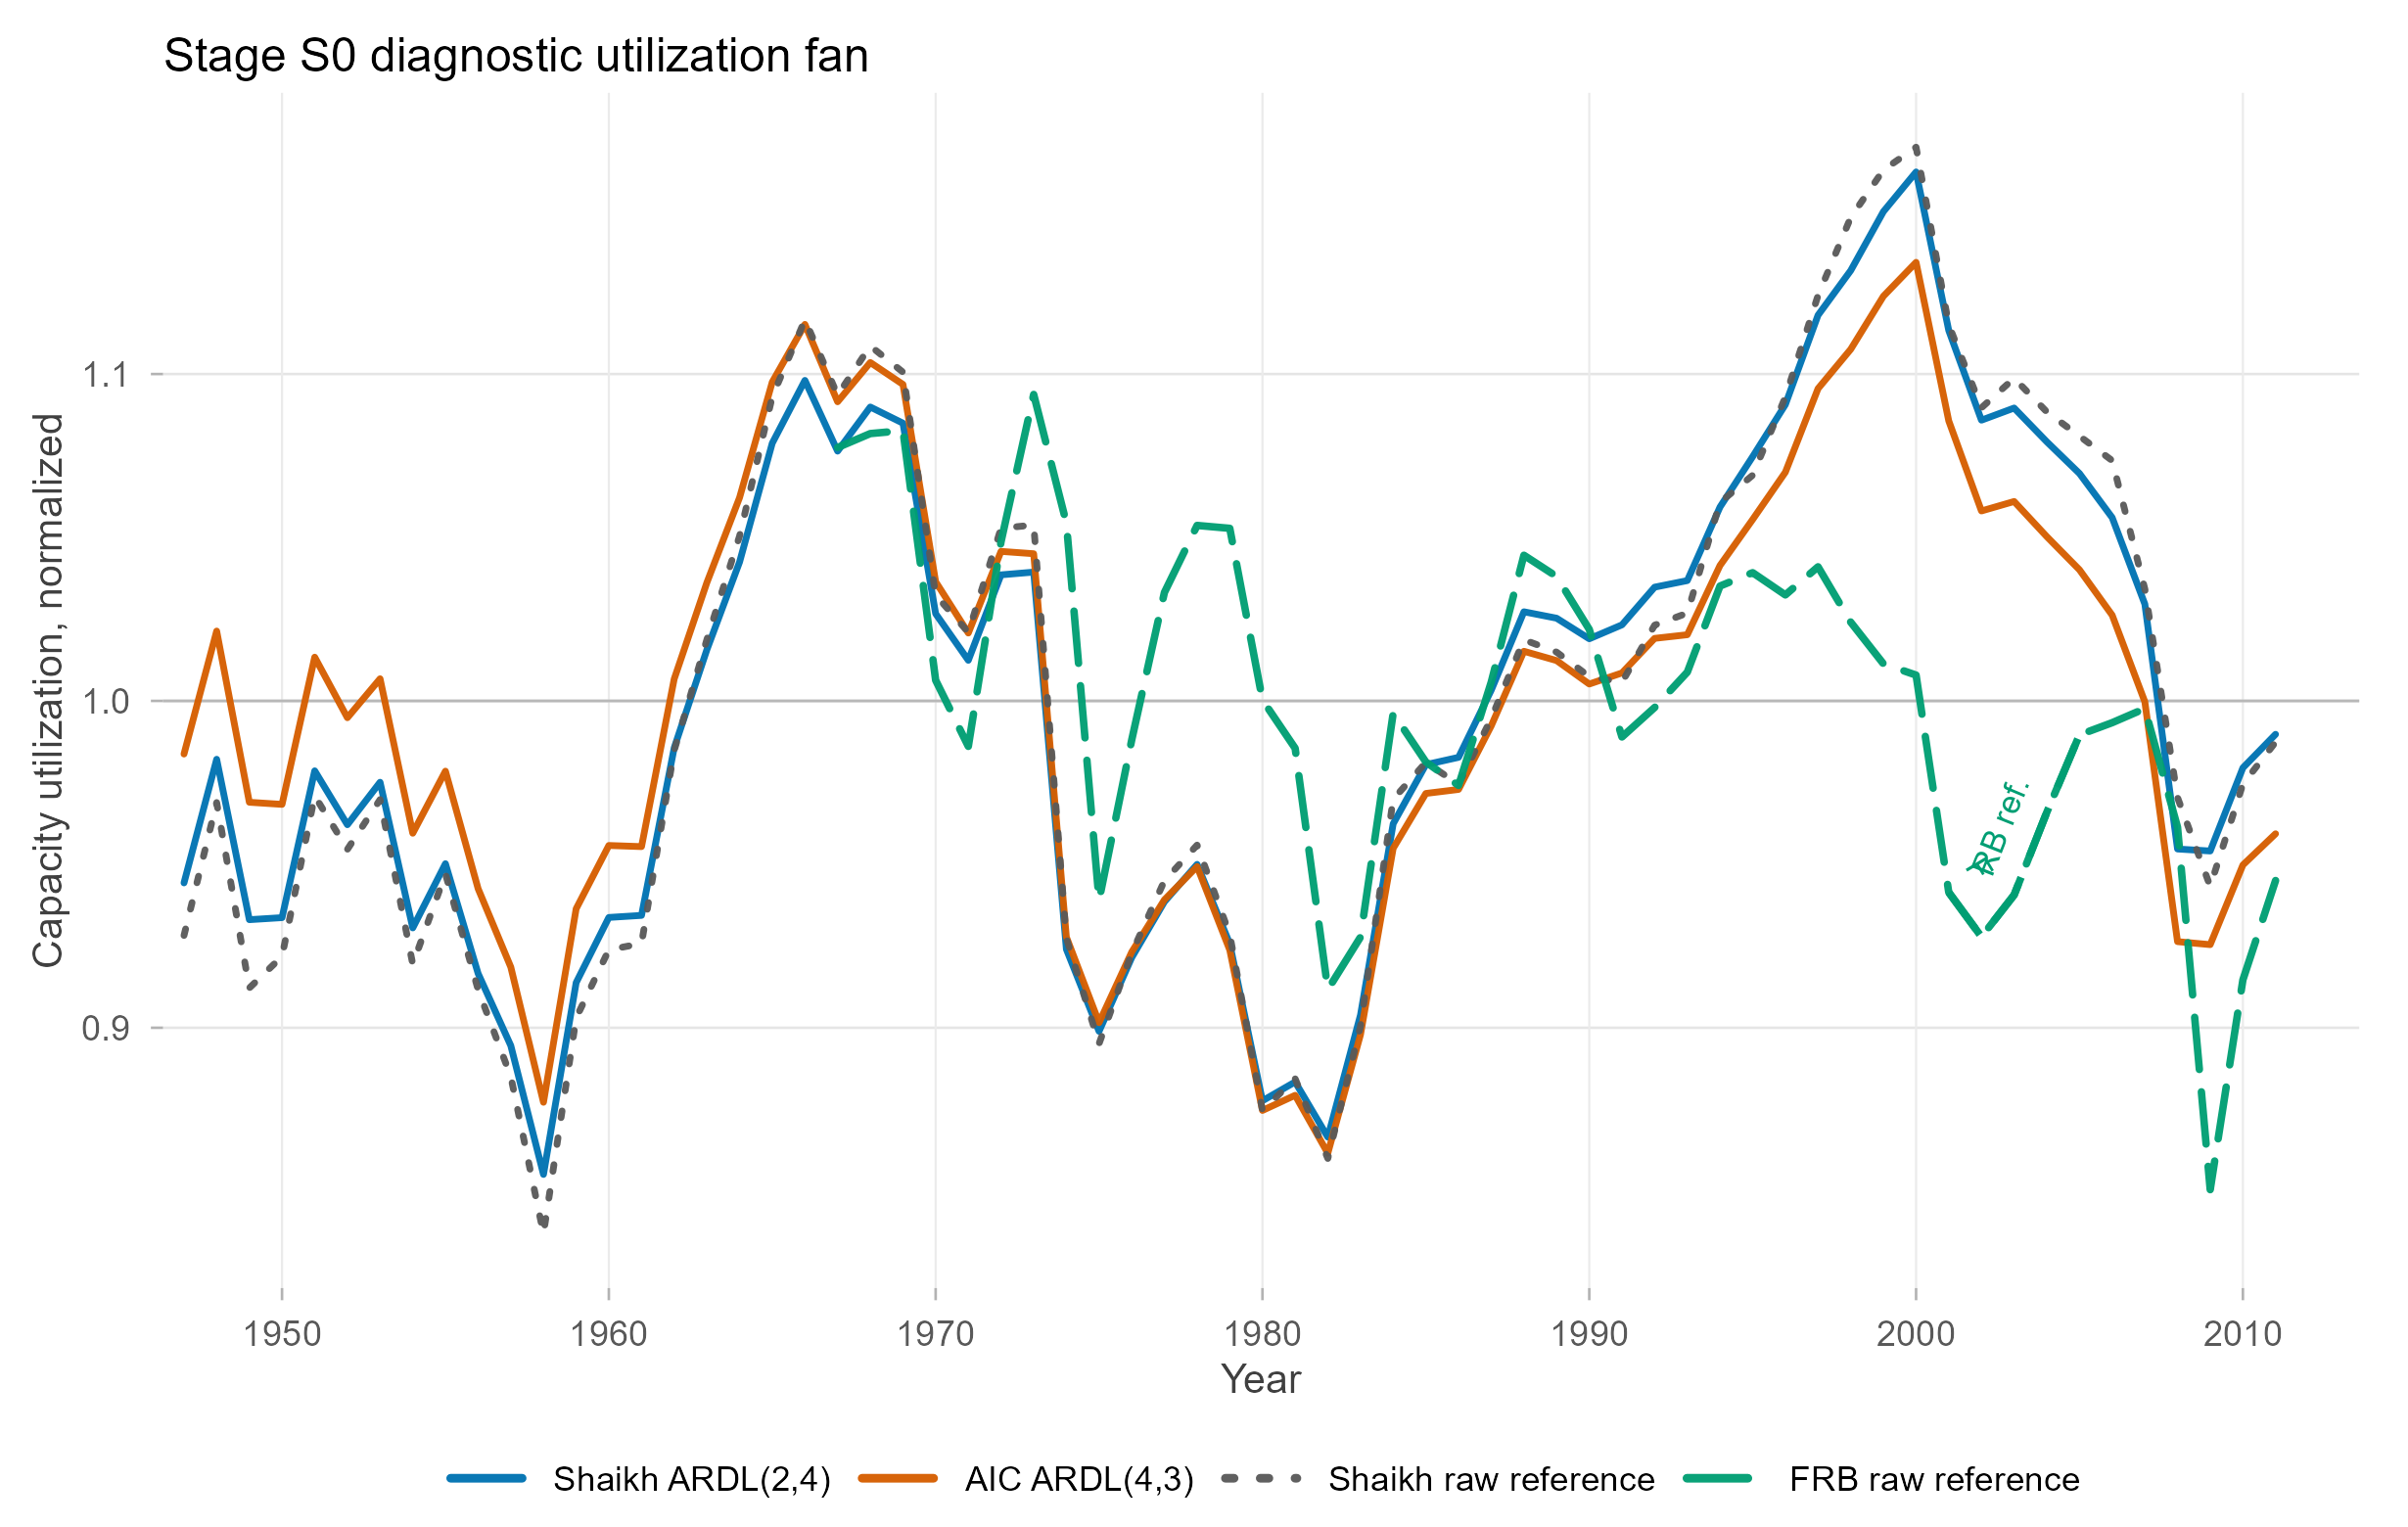
\includegraphics[width=0.92\linewidth]{figures/fig_S0_cu_fan_diagnostic.png}
\caption*{\footnotesize Note: All series are mean-normalized to unity over the 1947--2011 period. The solid blue line traces the reconstructed ARDL(2,4) specification ($\hat{\theta}=0.72$), the solid orange line traces the AIC-selected ARDL(4,3) specification ($\hat{\theta}=0.75$), the dashed grey line represents Shaikh's published series, and the dashed green line represents the normalized Federal Reserve Board manufacturing benchmark. Source: Author's elaboration.}
\end{figure}

The divergence between Shaikh's cointegrated index and the Federal Reserve Board series is also evident after 1973. While both series capture cyclical downturns (1958, 1974, 1982, and 2008), their secular trends differ. The FRB series is constructed from survey operating rates relative to existing plant capacity, which makes it mean-reverting around an 80\% operating rate. In contrast, Shaikh's measure reflects the output--capital relation across successive investment cycles. Because capital accumulation outpaced capacity expansion ($\hat{\theta} < 1$), the output--capital ratio fell after 1973, producing the persistent downward shift observed in Shaikh's utilization series. Recovering this baseline confirms that one can numerically reproduce a capacity path similar to Shaikh's. However, recovering a single point estimate does not establish that the parameter is unique across the specification space. To test this sensitivity, I transition to Stage S1 and estimate a broader grid of single-equation models.

\subsection{Stage 1 \texorpdfstring{$(S1)$}{}: Admissible-Specification Stress Test Results}
\label{subsec:S1_admissible_spec_new}

Expanding the analysis to a 500-model ARDL grid indicates that the estimated transformation elasticity is sensitive to specification choices. Rather than clustering tightly around a single value, the admissible estimates disperse across the parameter space: 102 of the 500 specifications pass the $F$-bounds test at the 10\% level, shrinking to 62 at 5\% and 13 at 1\%. Cointegration survival depends heavily on deterministic terms and historical controls: 92\% of the cointegrating specifications require at least one historical step control ($S_{1956}$, $S_{1974}$, or $S_{1980}$), and surviving models cluster predominantly in no-trend configurations. The bivariate output--capital relation does not cointegrate without these controls, and the recovered capacity path varies substantially with the selection of information criteria.

To illustrate this sensitivity, I compare two focal models that represent different regions of the specification space. The first is the model selected by AIC, BIC, HQ, and ICOMP: an ARDL(3,3) specification under PSS Case I (no constant, no trend) with the 1974 dummy, yielding an elasticity estimate of $\hat{\theta} = 0.920$ (SE 0.040). The second is the model selected by RICOMP: a parsimonious ARDL(1,2) specification under PSS Case II (restricted constant) with no dummies, yielding an elasticity estimate of $\hat{\theta} = 0.651$ (SE 0.070). Table~\ref{tab:s1_focal_parameters} reports the parameters and diagnostics for these two models.

\begin{table}[H]
\centering
\caption{Stage S1 Focal Single-Equation Estimations}
\label{tab:s1_focal_parameters}
\footnotesize
\begin{tabular}{lcccccc}
\toprule
& \multicolumn{3}{c}{AIC/BIC/HQ/ICOMP Focal: ARDL(3,3)} & \multicolumn{3}{c}{RICOMP Focal: ARDL(1,2)} \\
Parameter & Estimate & SE & $t$-stat & Estimate & SE & $t$-stat \\
\midrule
\midrule
$\hat{\theta}$ (elasticity) & 0.920 & 0.040 & 23.00$^{***}$ & 0.651 & 0.070 & 9.29$^{***}$ \\
$a$ (intercept) & \multicolumn{3}{c}{--- (Case 1)} & 0.584 & 0.402 & 1.45 \\
$S_{1974}$ & -0.038 & 0.017 & -2.24$^{**}$ & \multicolumn{3}{c}{--- ($s_0$)} \\
\midrule
$F$-bounds statistic & \multicolumn{3}{c}{8.120 (Case 1) [Reject $^{***}$]} & \multicolumn{3}{c}{3.269 (Case 2) [Reject $^{**}$]} \\
$t$-bounds statistic & \multicolumn{3}{c}{-4.520 (Case 1) [Reject $^{***}$]} & \multicolumn{3}{c}{-3.125 (Case 2) [Reject $^{**}$]} \\
$1 - \sum \alpha_i$ (denominator) & \multicolumn{3}{c}{0.240} & \multicolumn{3}{c}{0.091} \\
Breusch-Godfrey LM ($p$-value) & \multicolumn{3}{c}{0.48} & \multicolumn{3}{c}{0.39} \\
CUSUM/CUSUMSQ & \multicolumn{3}{c}{Stable} & \multicolumn{3}{c}{Stable} \\
\bottomrule
\end{tabular}
\caption*{\footnotesize Note: Small-sample critical values are simulated for $T=65$. Significance: $^{***}$ $p<0.01$, $^{**}$ $p<0.05$. Source: Author's elaboration.}
\end{table}

\begin{table}[H]
\centering
\caption{S1 Shrinking Specification Space Counts}
\label{tab:s1_shrinking_space_counts}
\small
\begin{tabular}{lr}
\toprule
Layer & Count \\
\midrule
\midrule
Full grid & 500 \\
Estimated successfully & 500 \\
F-admissible at 10\% & 102 \\
F+t confirmed at 10\% & 49 \\
F-admissible at 5\% & 62 \\
F+t confirmed at 5\% & 28 \\
F-admissible at 1\% & 13 \\
F+t confirmed at 1\% & 3 \\
$E_{S1}$ & 17 \\
IC-neighborhood union & 36 \\
\bottomrule
\end{tabular}
\caption*{\footnotesize Note: This table tracks the survival rate of the 500 estimated single-equation ARDL models through the nested cointegration admissibility gates. Source: Author's elaboration.}
\end{table}

Figure~\ref{fig:s1-shrinking-space-bounds-layers} visualizes this screening process. Panel A maps all 500 specifications across the fit-complexity space, color-coded by their cointegration status. Panel B tracks the number of surviving specifications at each diagnostic layer. This sequence reinforces the methodological principle of screening models for cointegration before evaluating relative fit or complexity.

\begin{figure}[H]
\centering
\caption{S1 Shrinking Specification Space}
\label{fig:s1-shrinking-space-bounds-layers}
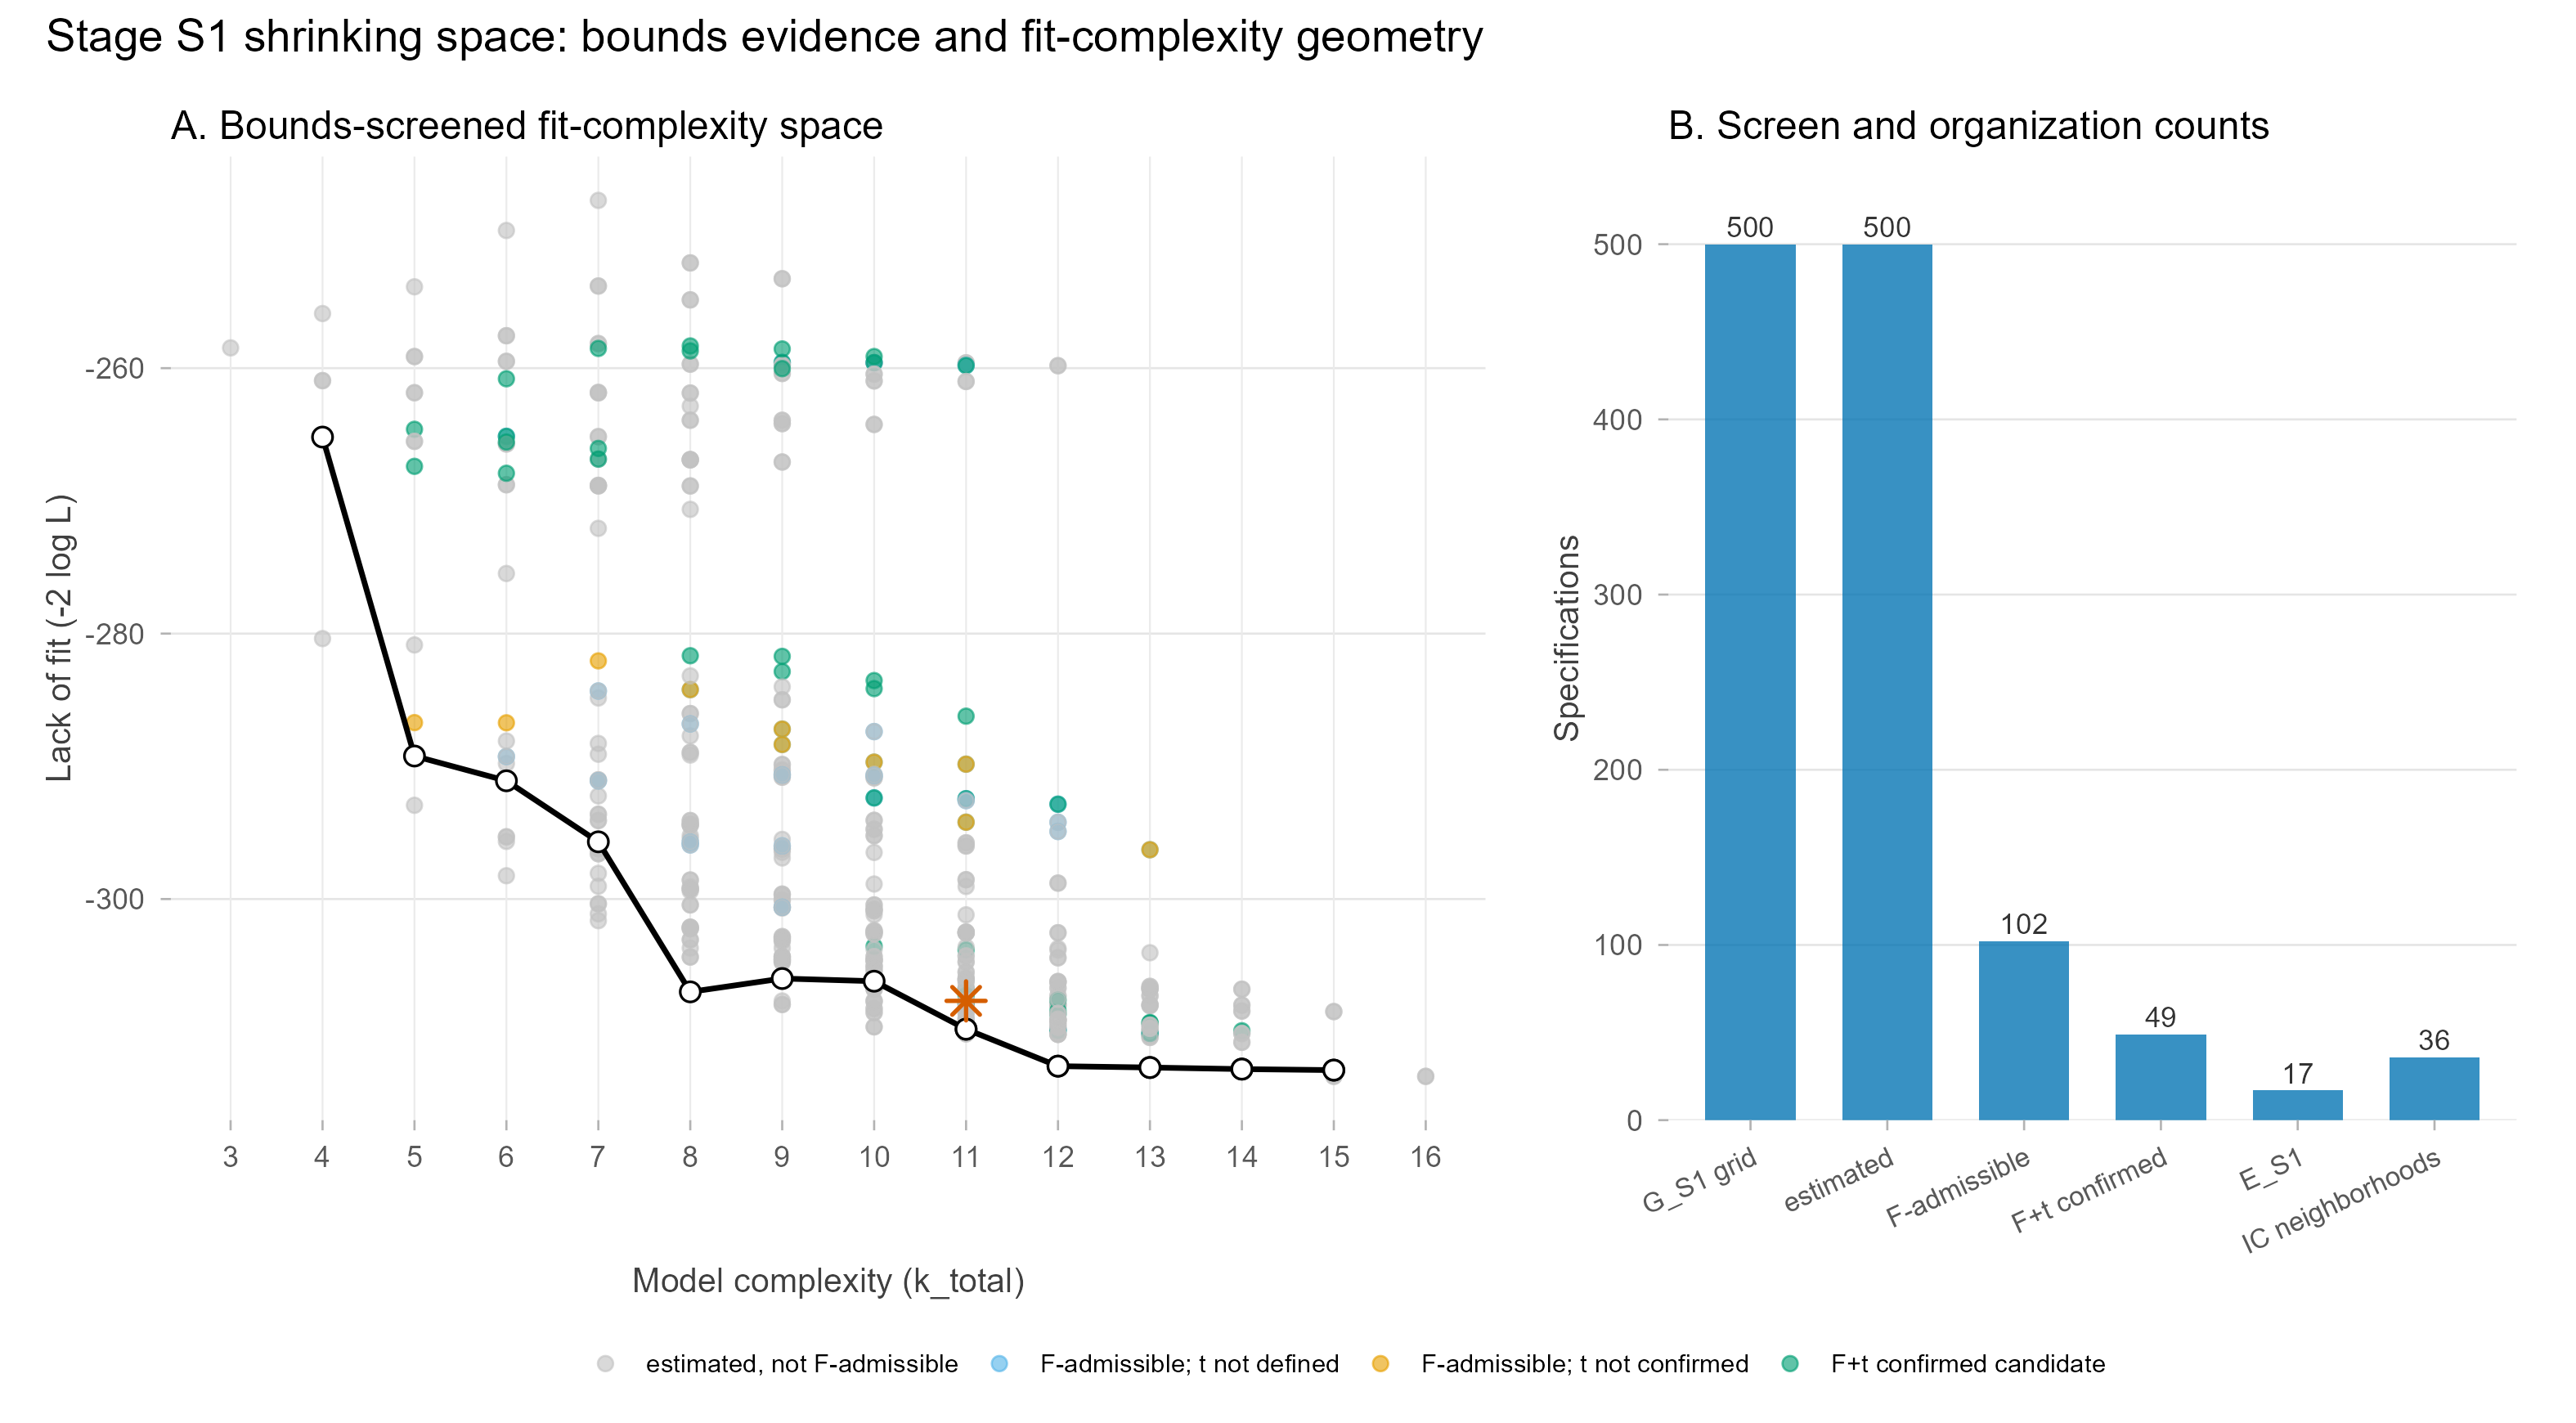
\includegraphics[width=0.92\linewidth]{figures/fig_S1_shrinking_space_bounds_layers.png}
\caption*{\footnotesize Source: Author's elaboration.}
\end{figure}

Within the cointegrating set, a fit--complexity envelope ($E_{S1}$) collects 17 Pareto-efficient specifications. This envelope represents the frontier along which model fit cannot be improved without increasing parameter count, nor simplified without worsening fit. The envelope provides a summary of the best-performing single-equation alternatives rather than selecting an individual preferred model.

The reliance on step controls ($S_{yy,t}$) reflects major disruptions in the post-war US economy: the 1956 post-Korean defense cuts, the 1974 OPEC oil price shock, and the 1980 Volcker interest rate shock. Bivariate models omitting these controls yield nonstationary residuals because these disruptions represent structural shifts in the output--capital relation. Restoring stationary errors requires these step controls to account for sudden downward adjustments in capital productivity ($Y/K$).

Information-criterion neighborhoods ($\mathcal{F}^{(0.20)}_j$) summarize the distribution of surviving models. For each criterion, the neighborhood collects the top 20\% of cointegrating specifications, resulting in a union of 36 unique models. Table~\ref{tab:s1_ic_neighborhood_summary} reports parameter ranges across these neighborhoods, illustrating how different selection criteria navigate the specification space.

\begin{table}[H]
\centering
\caption{S1 IC-Specific Neighborhood Summaries}
\label{tab:s1_ic_neighborhood_summary}
\small
\begin{tabular}{lrrrrr}
\toprule
Criterion & Specs & Min $\hat{\theta}$ & Mean $\hat{\theta}$ & Median $\hat{\theta}$ & Max $\hat{\theta}$ \\
\midrule
\midrule
AIC & 22 & 0.84 & 0.88 & 0.86 & 0.93 \\
BIC & 21 & 0.65 & 0.91 & 0.86 & 2.20 \\
HQ & 21 & 0.75 & 0.94 & 0.86 & 2.20 \\
ICOMP & 22 & 0.65 & 0.84 & 0.86 & 0.95 \\
RICOMP & 22 & 0.65 & 0.83 & 0.85 & 0.95 \\
\bottomrule
\end{tabular}
\caption*{\footnotesize Note: The table reports the summary statistics for the long-run parameter $\hat{\theta}$ within the bottom 20th percentile of each information criterion. Estimates are rounded to two decimal places for consistency. Source: Author's elaboration.}
\end{table}

Figure~\ref{fig:s1-crossed-frontier-ic-neighborhoods} maps these criterion neighborhoods against the fit-complexity envelope. The solid line represents the Pareto frontier ($E_{S1}$), while the shaded areas show the neighborhoods for each criterion, highlighting the spatial divergence between the parsimonious models selected by RICOMP and the higher-order models selected by AIC and BIC.

\begin{figure}[H]
\centering
\caption{S1 Fit--Complexity Envelope and IC-Specific Neighborhoods}
\label{fig:s1-crossed-frontier-ic-neighborhoods}
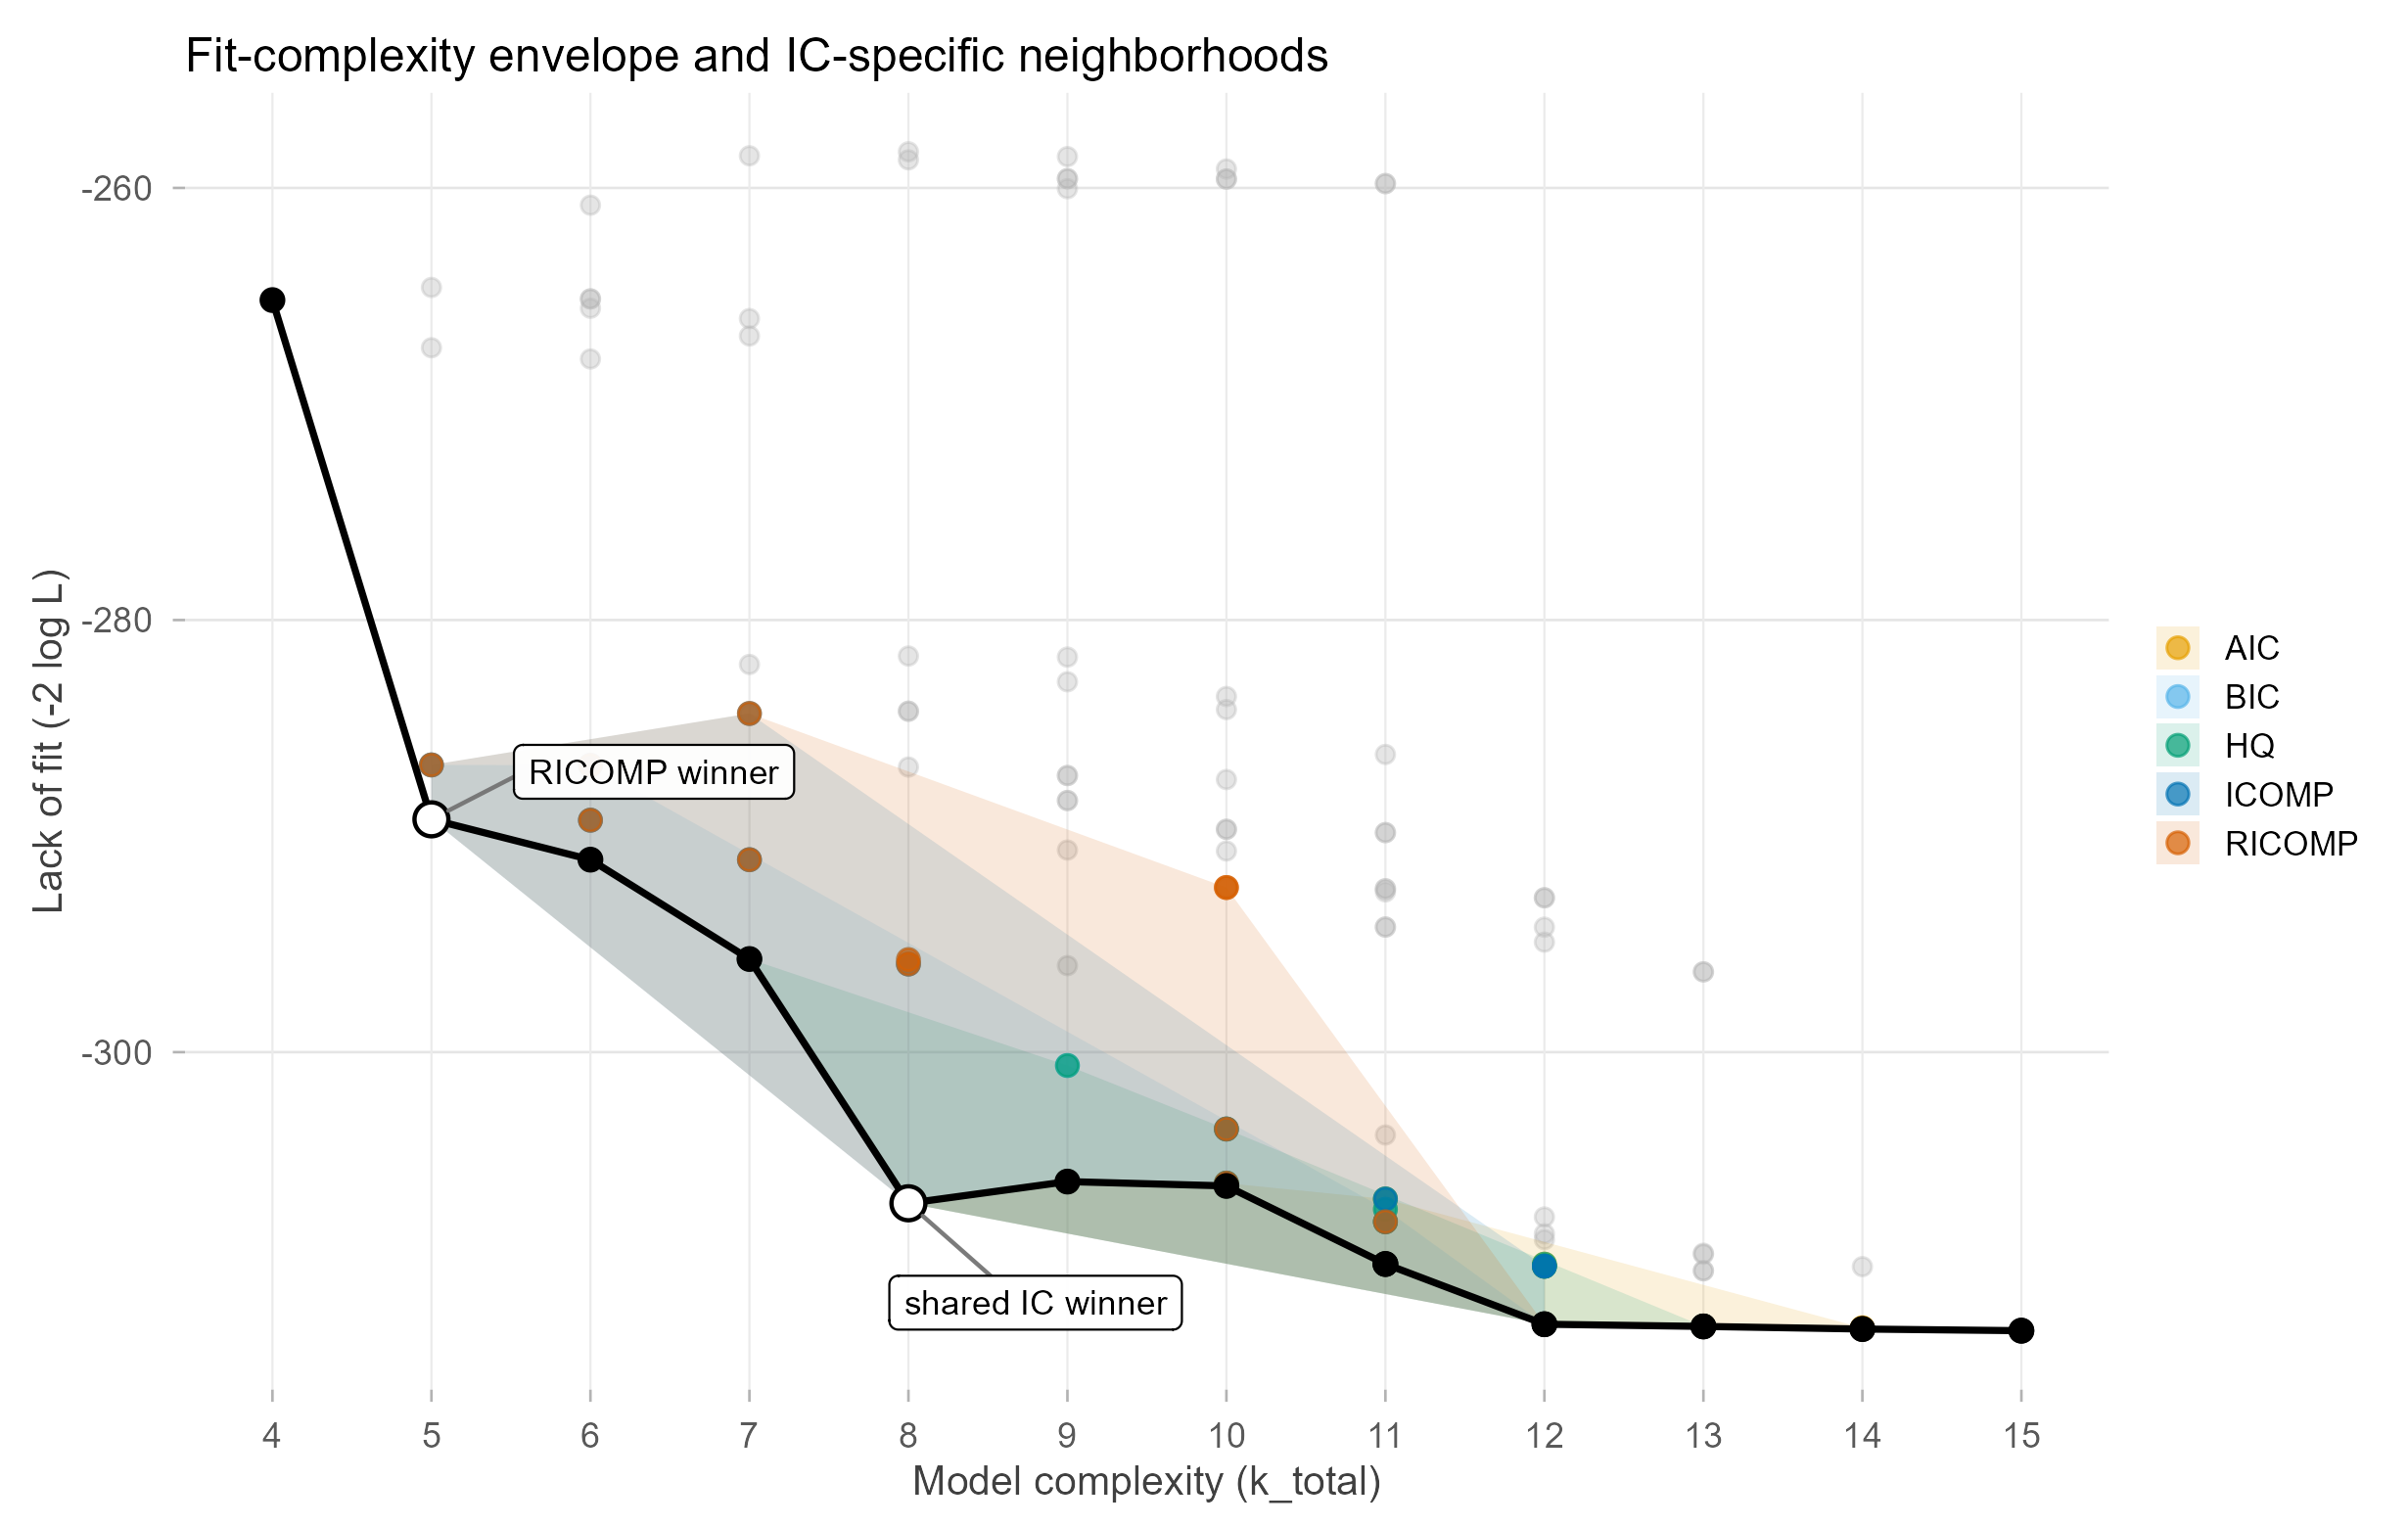
\includegraphics[width=0.92\linewidth]{figures/fig_S1_global_frontier_IC_neighborhoods.png}
\caption*{\footnotesize Source: Author's elaboration.}
\end{figure}

This divergence demonstrates that alternative information-theoretic penalties identify distinct areas of the specification space. AIC and BIC penalize parameter counts, selecting the ARDL(3,3) model with $\hat{\theta}=0.920$. In contrast, ICOMP and RICOMP penalize parameter covariance complexity, selecting the parsimonious ARDL(1,2) model with $\hat{\theta}=0.651$. This dispersion has direct substantive implications. In no-trend configurations (PSS Cases I, II, and III), surviving elasticities lie below unity ($\hat{\theta} \in [0.65, 0.95]$), consistent with an overaccumulation regime. Conversely, trend-containing configurations (Cases IV and V) produce elasticities averaging 1.36 and reaching up to 2.20. An elasticity $\theta > 1$ implies that productive capacity expands faster than the capital stock in the long run. I exclude these trend-containing specifications not on purely statistical grounds, but because they generate economically implausible capacity trajectories.

Figure~\ref{fig:s1-cu-fan-ic-neighborhoods} plots the utilization paths generated by these different cointegrating models. The shaded fan displays the dispersion of constructed capacity utilization, while the divergent paths of the AIC and RICOMP selections illustrate how model choice affects historical measures of capacity realization.

To examine the implications of assuming balanced growth, I estimate a counterfactual specification imposing $\theta = 1.0$, requiring capacity to grow proportionally with capital. Under this restriction, the implied capacity utilization index drifts downward to under 35\% for extended periods and exceeds 105\% during cyclical peaks. Such an index implies prolonged operational rates incompatible with observed corporate survival, indicating that imposing a unitary elasticity is ill-suited to this data construction. Estimating $\theta$ freely is therefore necessary to generate an economically coherent utilization series.

\begin{figure}[H]
\centering
\caption{S1 Diagnostic Utilization Fan from IC-Specific Neighborhoods}
\label{fig:s1-cu-fan-ic-neighborhoods}
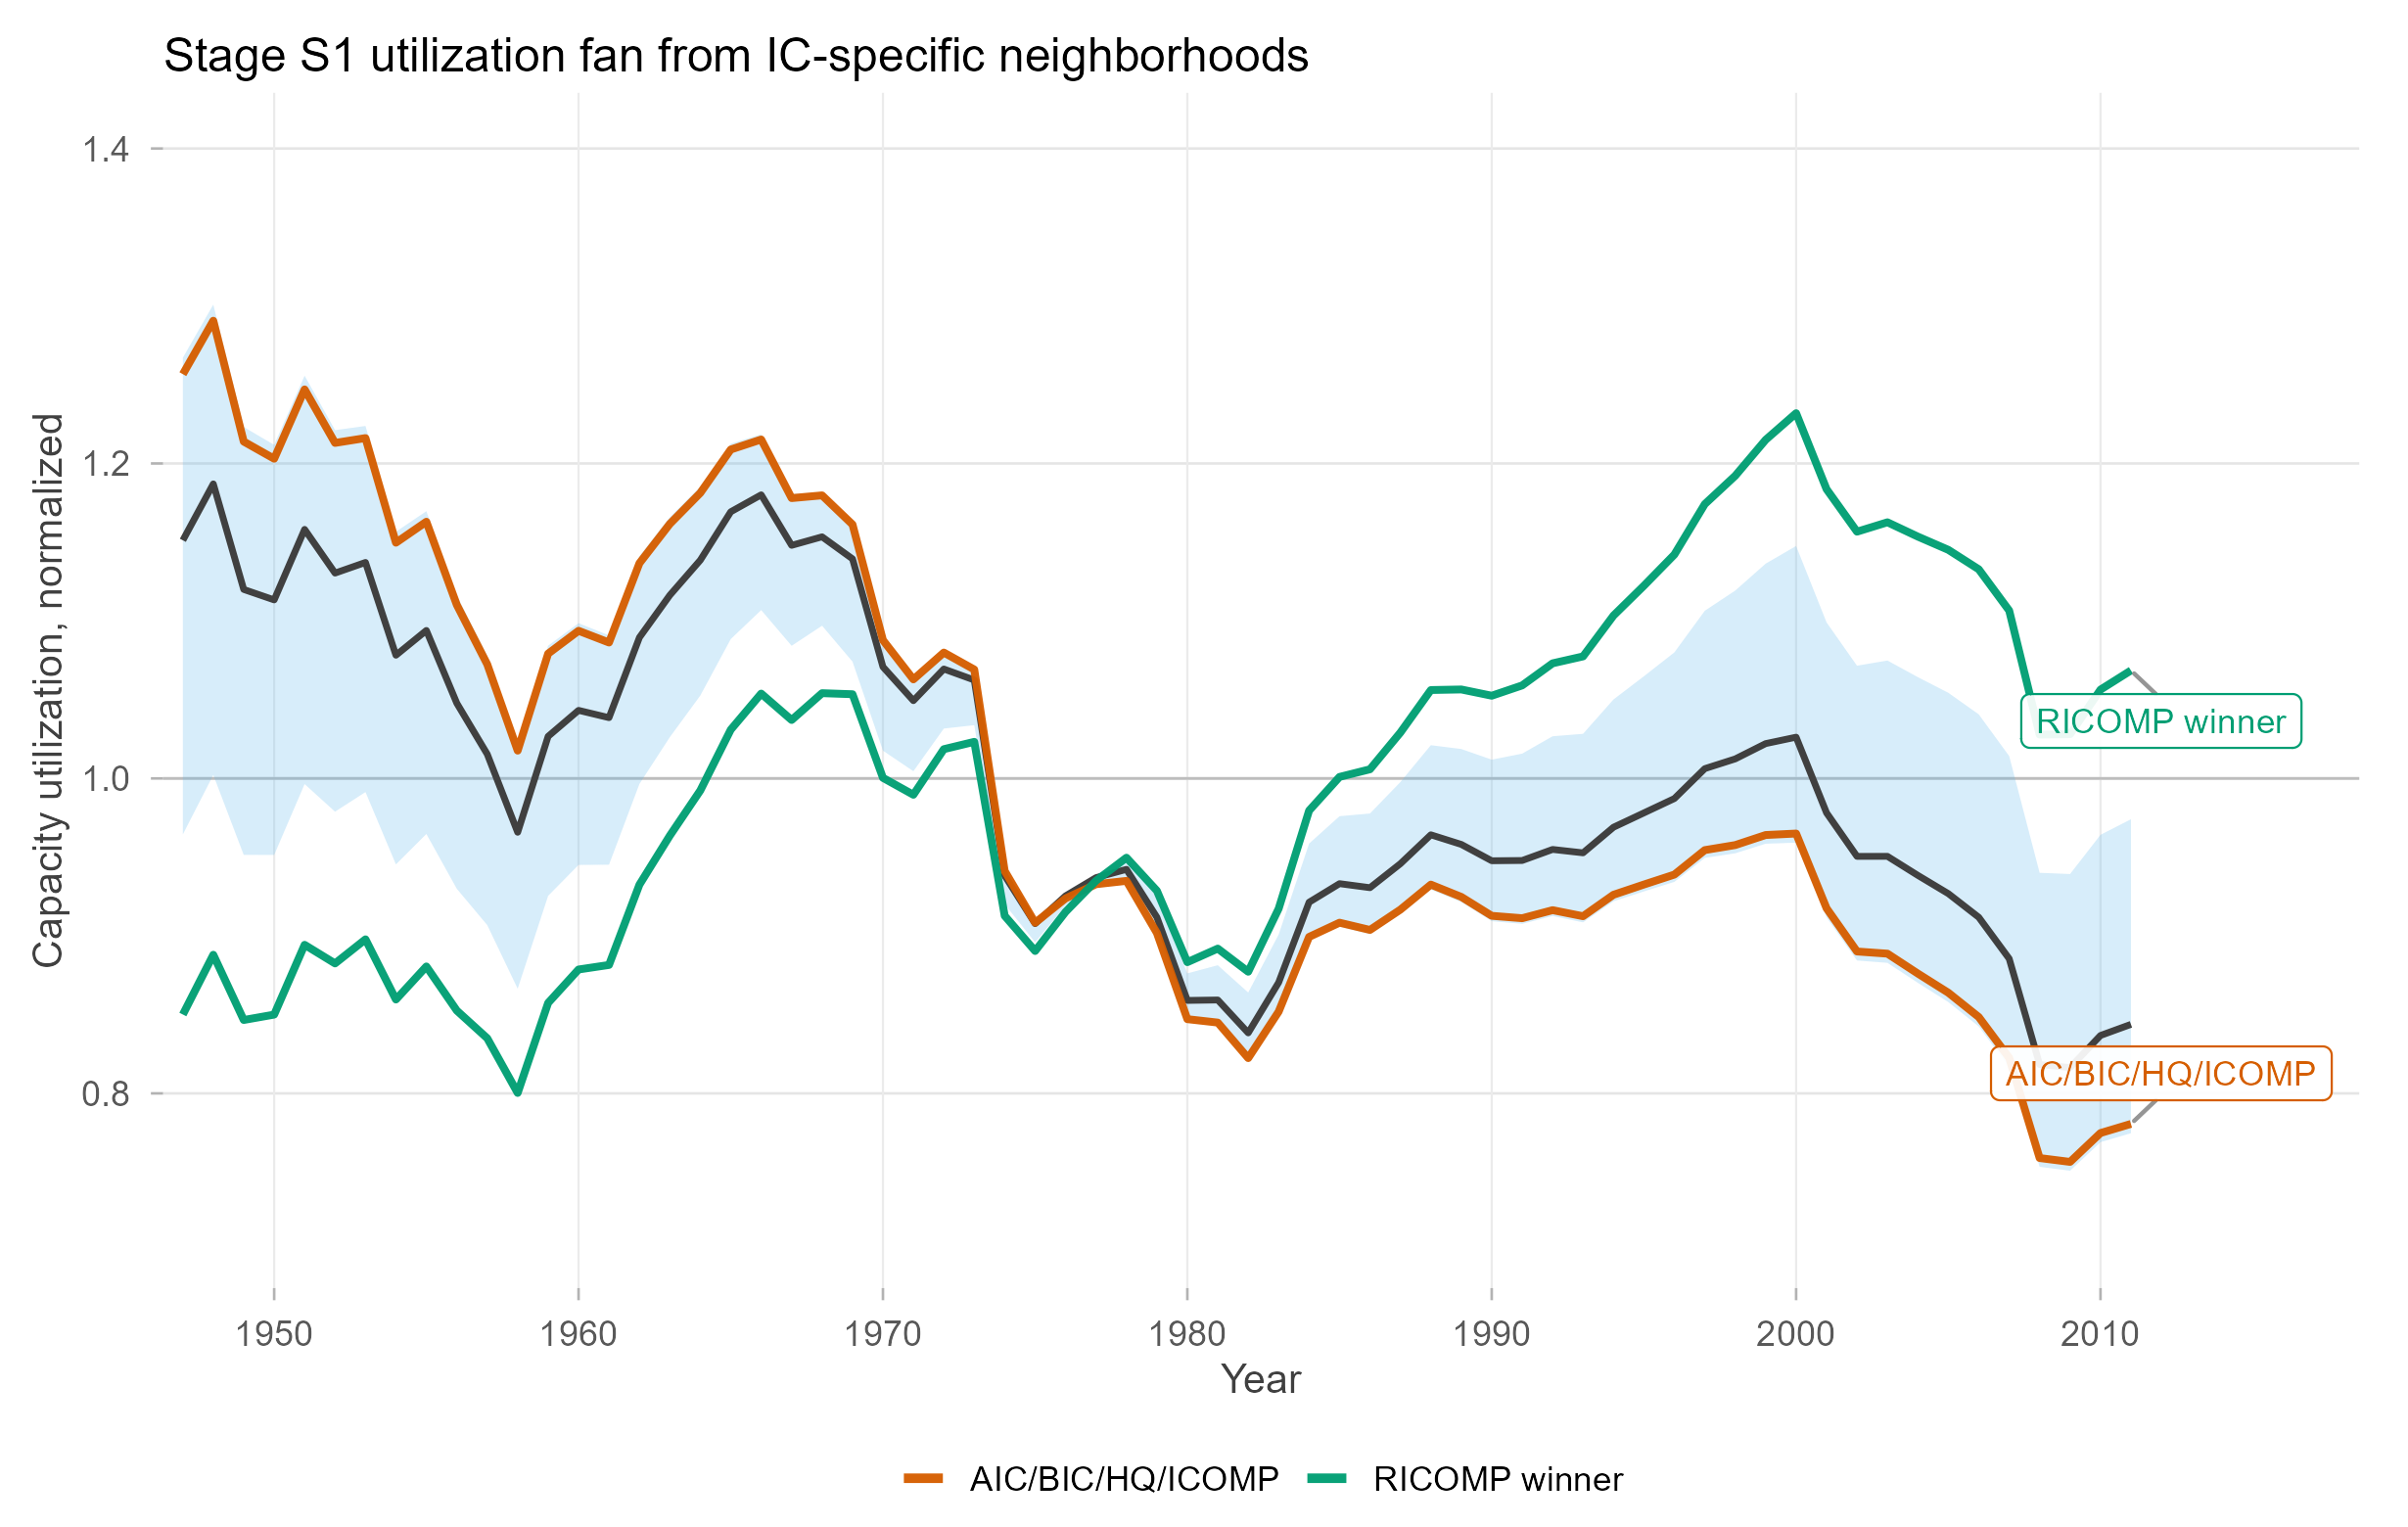
\includegraphics[width=0.92\linewidth]{figures/fig_S1_cu_fan_IC_neighborhoods.png}
\caption*{\footnotesize Source: Author's elaboration.}
\end{figure}

Stage S1 demonstrates that while multiple single-equation specifications satisfy cointegration bounds tests, they generate divergent estimates of the transformation elasticity ($\hat{\theta} \in [0.65, 0.95]$). Because the single-equation framework does not identify a unique parameter value, capacity paths constructed from this approach remain specification-dependent. In Subsection~\ref{subsec:S2_vecm}, I examine whether the output--capital relation achieves greater stability within a multi-equation VECM framework, and whether system cointegration requires the inclusion of functional income distribution.

\subsection{Stage 2 \texorpdfstring{$(S2)$}{}: System-Level VECM Replication}
\label{subsec:S2_vecm}

Evaluating the output--capital relation within a system-level Vector Error Correction Model (VECM) exposes the econometric limits of the single-equation framework. Across 48 attempted bivariate specifications (36 successfully estimated) sweeping lag orders and deterministic configurations over the 1947--2011 sample, the bivariate system yields zero cointegrating relationships. Residuals remain non-stationary ($I(1)$). This breakdown demonstrates that capital accumulation and output cannot sustain a stable long-run trajectory in isolation. Long-run system stability becomes recoverable only when the rate of exploitation enters the state vector alongside historical step controls.

Because the bivariate system yields non-stationary residuals over the full post-war sample, estimating the output--capital relation requires including income distribution in the state vector. I incorporate the rate of exploitation, defined in Shaikh's corporate accounts as corporate net operating surplus relative to employee compensation ($e_t = \Pi_t / W_t = \text{NOScorp}_t / \text{ECcorp}_t$). In logarithms, this variable links directly to the profit share ($\pi_t \equiv \Pi_t / Y_t$) and the wage share ($\omega_t \equiv W_t / Y_t = 1 - \pi_t$):
\begin{equation}
\label{eq:exploitation_log_odds}
\ln e_t = \ln \left( \frac{\pi_t}{1 - \pi_t} \right) = \ln \pi_t - \ln \omega_t.
\end{equation}
Econometrically, $\ln e_t$ is a continuous log-odds transform of functional distribution. It maps the bounded wage share $\omega_t \in (0, 1)$ onto the real line $(-\infty, +\infty)$, avoiding the boundary constraints that can distort linear vector error correction models. Furthermore, incorporating distribution through $\ln e_t$ avoids the collinearity that arises if the profit rate $r_t = \pi_t (Y_t / K_t)$ is entered alongside $\ln Y_t$ and $\ln K_t$.

I summarize these system-level outcomes in Table~\ref{tab:s2_admissibility_outcomes}. All 48 attempted bivariate specifications (36 successfully estimated) fail to cointegrate. In contrast, the trivariate family yields six admissible models at rank $r=1$ when the rate of exploitation and historical step controls enter the system. These results demonstrate that the output--capital relation achieves system stability only when conditioned on functional distribution.

\begin{table}[H]
\centering
\caption{S2 System Admissibility Outcomes}
\label{tab:s2_admissibility_outcomes}
\footnotesize
\begin{tabular}{@{}>{\raggedright\arraybackslash}p{3.6cm}crrr>{\raggedright\arraybackslash}p{4.4cm}@{}}
\toprule
System & Rank & Attempted & Estimated & Admissible & Interpretation \\
\midrule
\midrule
Bivariate $(\ln Y,\ln K)$ & $r=1$ & 48 & 36 & 0 & Output--capital relation is not self-sufficient \\
Trivariate $(\ln Y,\ln K,\ln e)$ & $r=1$ & 48 & 36 & 6 & Restricted survival with logged exploitation \\
Trivariate $(\ln Y,\ln K,\ln e)$ & $r=2$ & 48 & 36 & 0 & No admissible two-vector system \\
\bottomrule
\end{tabular}
\caption*{\footnotesize Note: Each system-rank block specifies 48 attempted configurations ($4\text{ lags} \times 4\text{ deterministic branches} \times 3\text{ dummy sets}$). In all three blocks, exactly 12 specifications under deterministic branch $C_1$ (restricted constant in cointegrating space) failed numerical convergence in \texttt{tsDyn}, yielding 36 successfully estimated specifications per block (108 total across all three blocks). Source: Author's elaboration.}
\end{table}

To ground the VECM results, I select the VAR(2) specification under Johansen Case 3 ($C_2$: unrestricted short-run constant absorbing linear drift in levels), $h_2$ step controls ($S_{yy,t}$), and rank $r=1$ as the focal model. The model satisfies the mechanical triple admissibility gate: (1) numerical convergence, (2) rejection of $r=0$ at the 5\,\% level with failure to reject $r \leq 1$ in the Johansen trace test (Trace statistic $32.28 > 31.52$; $10.68 < 17.95$), and (3) companion matrix dynamic stability with all non-unit roots strictly inside the unit circle (eigenvalue moduli $1.0, 1.0, 0.82, 0.52, 0.52, 0.49$, exhibiting exactly $m - r = 2$ unit roots).

Subsequent diagnostic quality screens confirm multivariate normality (Jarque--Bera statistic $5.72$, $p=0.456$), absence of autoregressive conditional heteroskedasticity (ARCH-LM(4) statistic $150.03$, $p=0.348$), and absence of higher-order Portmanteau autocorrelation (Portmanteau(12) statistic $100.70$, $p=0.275$). While the Breusch--Godfrey LM(4) statistic is $60.81$ ($p=0.006$), reflecting lag-4 sensitivity in a small macroeconomic sample ($T=65$) with multiple exogenous step indicators, this does not invalidate the superconsistent Johansen ML estimates, though it qualifies claims of absolute residual whitening and warrants transparent reporting.

Normalized on output, the estimated cointegrating vector is:
\begin{equation}
\ln Y_t = 0.727 \ln K_t - 20.022 \ln e_t + c_0 + \hat{\varepsilon}_t.
\label{eq:s2_cointegrating_vector}
\end{equation}
The estimated transformation elasticity ($\hat{\theta} = 0.727$, $\text{SE} = 4.852$, $t = -0.15$) is numerically close to the reconstructed single-equation baseline ($\hat{\theta} \approx 0.720$), but carries substantial estimation uncertainty. In sharp contrast, the coefficient on the rate of exploitation is identified with high precision ($\hat{\beta}_e = 20.022$, $\text{SE} = 2.536$, $t = 7.90$, $p < 0.001$). An inspection of the empirical variances of the cointegrating components clarifies this structural asymmetry: the unadjusted marginal variance ratio for the exploitation term, $\text{Var}(20.022 \ln e_t)/\text{Var}(\hat{\beta}' X_t)$, is 99.1\,\%, whereas the output and capital marginal ratios contribute 5.6\,\% and 5.0\,\% respectively. These individual marginal ratios sum to 109.7\,\% because they do not constitute orthogonal variance shares, omitting the substantial negative sample covariance between co-trending output and capital ($\text{Cov}(\ln Y_t, -0.727 \ln K_t) < 0$). Rather than establishing an additive variance partition, this asymmetry highlights that the rate of exploitation anchors the cointegrating vector with high parameter precision, whereas the capital-output transformation elasticity carries substantial normalized uncertainty.

To interpret the economic mechanism implied by this vector, I write the relation in its reserve-army form by renormalizing on $\ln e_t$:
\begin{equation}
\label{eq:focal_vecm_reserve_army}
\ln e_t = -0.050 \, \left(\ln Y_t - 0.727 \ln K_t\right) + c + \hat{v}_t.
\end{equation}
The term $(\ln Y_t - 0.727 \ln K_t)$ represents capacity utilization disequilibrium. The estimated elasticity of $-0.050$ reflects a reserve-army feedback: when the economy operates above normal capacity ($\ln Y_t > 0.727 \ln K_t$), labor market tightening dampens the exploitation rate, raising the wage share. When excess capacity develops, unemployment relieves wage pressure, restoring the exploitation rate. At the system level, capacity utilization and distribution adjust jointly within a single cointegrating relationship.

The adjustment loading vector ($\alpha$) indicates a pronounced structural asymmetry. In the capital equation, the estimated error-correction loading is statistically indistinguishable from zero ($\hat{\alpha}_k = 0.0003$, $t = 0.92, p = 0.360$), indicating that capital accumulation does not adjust to eliminate cointegrating disequilibrium. Output adjusts modestly ($\hat{\alpha}_y = -0.005$, $t = -2.00, p = 0.050$), while the primary burden of error correction falls on the rate of exploitation ($\hat{\alpha}_e = -0.019$, $t = -4.25, p < 0.001$). This pattern reflects a slow, structural adjustment channel operating primarily through income distribution. While the near-zero adjustment of capital ($\hat{\alpha}_k \approx 0$) is suggestively consistent with classical-Sraffian models where capital accumulation is autonomous, it cannot be interpreted as a formal statistical rejection of Neo-Kaleckian closure without a joint likelihood-ratio restriction test. What the system establishes is that the return to the long-run attractor is mediated through distributional compression rather than rapid capital stock adjustments. I report the short-run dynamics ($\Gamma_1$) and deterministic step coefficients ($\Phi$) in Table~\ref{tab:s2_short_run_dynamics}.

\begin{table}[H]
\centering
\caption{Focal VECM Short-Run Dynamics and Step Controls}
\label{tab:s2_short_run_dynamics}
\footnotesize
\begin{tabular}{lccc}
\toprule
Regressor / Control & $\Delta \ln Y_t$ Equation & $\Delta \ln K_t$ Equation & $\Delta \ln e_t$ Equation \\
\midrule
\midrule
$\Delta \ln Y_{t-1}$ & 0.199 (0.150) & 0.047$^{**}$ (0.023) & -0.798$^{**}$ (0.314) \\
$\Delta \ln K_{t-1}$ & -1.015 (0.564) & 0.812$^{***}$ (0.087) & -4.023$^{***}$ (1.183) \\
$\Delta \ln e_{t-1}$ & -0.023 (0.067) & 0.015 (0.010) & -0.069 (0.140) \\
\midrule
$S_{1956}$ (step indicator) & -0.005 (0.015) & 0.002 (0.002) & -0.062$^{**}$ (0.029) \\
$S_{1974}$ (step indicator) & -0.038$^{**}$ (0.017) & 0.001 (0.002) & -0.078$^{**}$ (0.032) \\
$S_{1980}$ (step indicator) & 0.001 (0.016) & -0.003 (0.002) & -0.014 (0.031) \\
\bottomrule
\end{tabular}
\caption*{\footnotesize Note: Standard errors are in parentheses. Significance: $^{***}$ $p<0.01$, $^{**}$ $p<0.05$. Source: Author's elaboration.}
\end{table}

The six surviving trivariate models require a clear two-tier taxonomy that distinguishes mechanical statistical admissibility from deterministic modeling adequacy (Table~\ref{tab:s2_retained_trivariate_specs}). All six specifications satisfy the Tier 1 statistical gate (convergence, trace rank test rejection of $r=0$ at 5\,\%, and companion matrix dynamic stability). However, their economic plausibility varies systematically across deterministic branches:
\begin{enumerate}[label=(\roman*)]
\item \textbf{Preferred Deterministic Branch ($C_2$, Tier 2):} Macroeconomic levels exhibit secular linear growth, requiring an unrestricted short-run constant in differences to absorb linear drift without forcing deterministic trends into the long-run cointegrating relationship. Both surviving specifications on this branch ($p=1, \hat{\theta}=0.97$; and focal $p=2, \hat{\theta}=0.73$) generate transformation elasticities inside the structural overaccumulation interval ($0 < \hat{\theta} < 1$).
\item \textbf{Zero-Constant Branch ($C_0$, Tier 1):} By omitting deterministic constants entirely, these models force secular drift into the cointegrating vector, leading to drift-distorted parameter estimates in higher-order dynamics ($p=1, \hat{\theta}=0.91$; and $p=2, \hat{\theta}=1.19$).
\item \textbf{Saturated Trend Branch ($C_3$, Inadmissible):} Saturated linear trends in differences overparameterize the small sample ($T=65$), causing the deterministic trend to absorb output growth and yielding pathological elasticities ($\hat{\theta} = -0.81$ and $\hat{\theta} = 11.31$).
\end{enumerate}

\begin{table}[H]
\centering
\caption{S2 Retained Trivariate Specifications and Disposition Taxonomy}
\label{tab:s2_retained_trivariate_specs}
\footnotesize
\begin{tabular}{@{}>{\raggedright\arraybackslash}p{2.4cm}cccr>{\raggedright\arraybackslash}p{5.8cm}@{}}
\toprule
Spec ID & Lag ($p$) & Det.\ Case & Dummies & $\hat{\theta}$ & Evaluation / Role \\
\midrule
\midrule
\texttt{p1\_d0\_h2\_r1} & 1 & $C_0$ & $h_2$ & 0.91 & Tier 1 statistical survivor (unmodeled drift) \\
\texttt{p1\_d2\_h2\_r1} & 1 & $C_2$ & $h_2$ & 0.97 & Tier 2: Preferred deterministic branch ($C_2$; drift absorption; $\hat{\theta} < 1.0$) \\
\texttt{p1\_d3\_h2\_r1} & 1 & $C_3$ & $h_2$ & -0.81 & Inadmissible (trend overparameterization) \\
\texttt{p2\_d0\_h2\_r1} & 2 & $C_0$ & $h_2$ & 1.19 & Tier 1 statistical survivor (BIC winner; $\hat{\theta} > 1$) \\
\texttt{p2\_d2\_h2\_r1} & 2 & $C_2$ & $h_2$ & 0.73 & Tier 2: Focal specification ($C_2$; drift absorption; $\hat{\theta} = 0.73$) \\
\texttt{p2\_d3\_h2\_r1} & 2 & $C_3$ & $h_2$ & 11.31 & Inadmissible (AIC winner; trend overparameterization) \\
\bottomrule
\end{tabular}
\caption*{\footnotesize Note: All specifications possess rank $r=1$. Tier 1 models pass Johansen rank and stability tests. Tier 2 models are selected ex-ante on deterministic grounds ($C_2$ absorbing linear secular drift), yielding sub-unitary elasticities. Source: Author's elaboration.}
\end{table}

Historical step controls ($S_{1956}, S_{1974}, S_{1980}$) are essential for establishing system-level cointegration. Cointegration holds only when the model includes step controls to absorb permanent structural breaks, preventing permanent mean shifts in residuals from appearing as unit roots. When these shock controls are omitted ($h_0$ counterfactual), the VECM fails to reject the null of no cointegration under both Johansen trace and maximum eigenvalue tests across all lag orders. Output, capital, and exploitation drift apart permanently without a restoring attractor. System stability depends on controlling for major post-war shocks: the 1956 capital deepening threshold, the 1974 oil and profitability crisis, and the 1980 Volcker monetary tightening.

I plot the system-level fit-complexity frontier in Figure~\ref{fig:s2-pooled-frontier}. Bivariate systems fail to cointegrate, while trivariate systems with logged exploitation achieve admissibility under disciplined historical controls.

\begin{figure}[H]
\centering
\caption{S2 Pooled System Frontier}
\label{fig:s2-pooled-frontier}
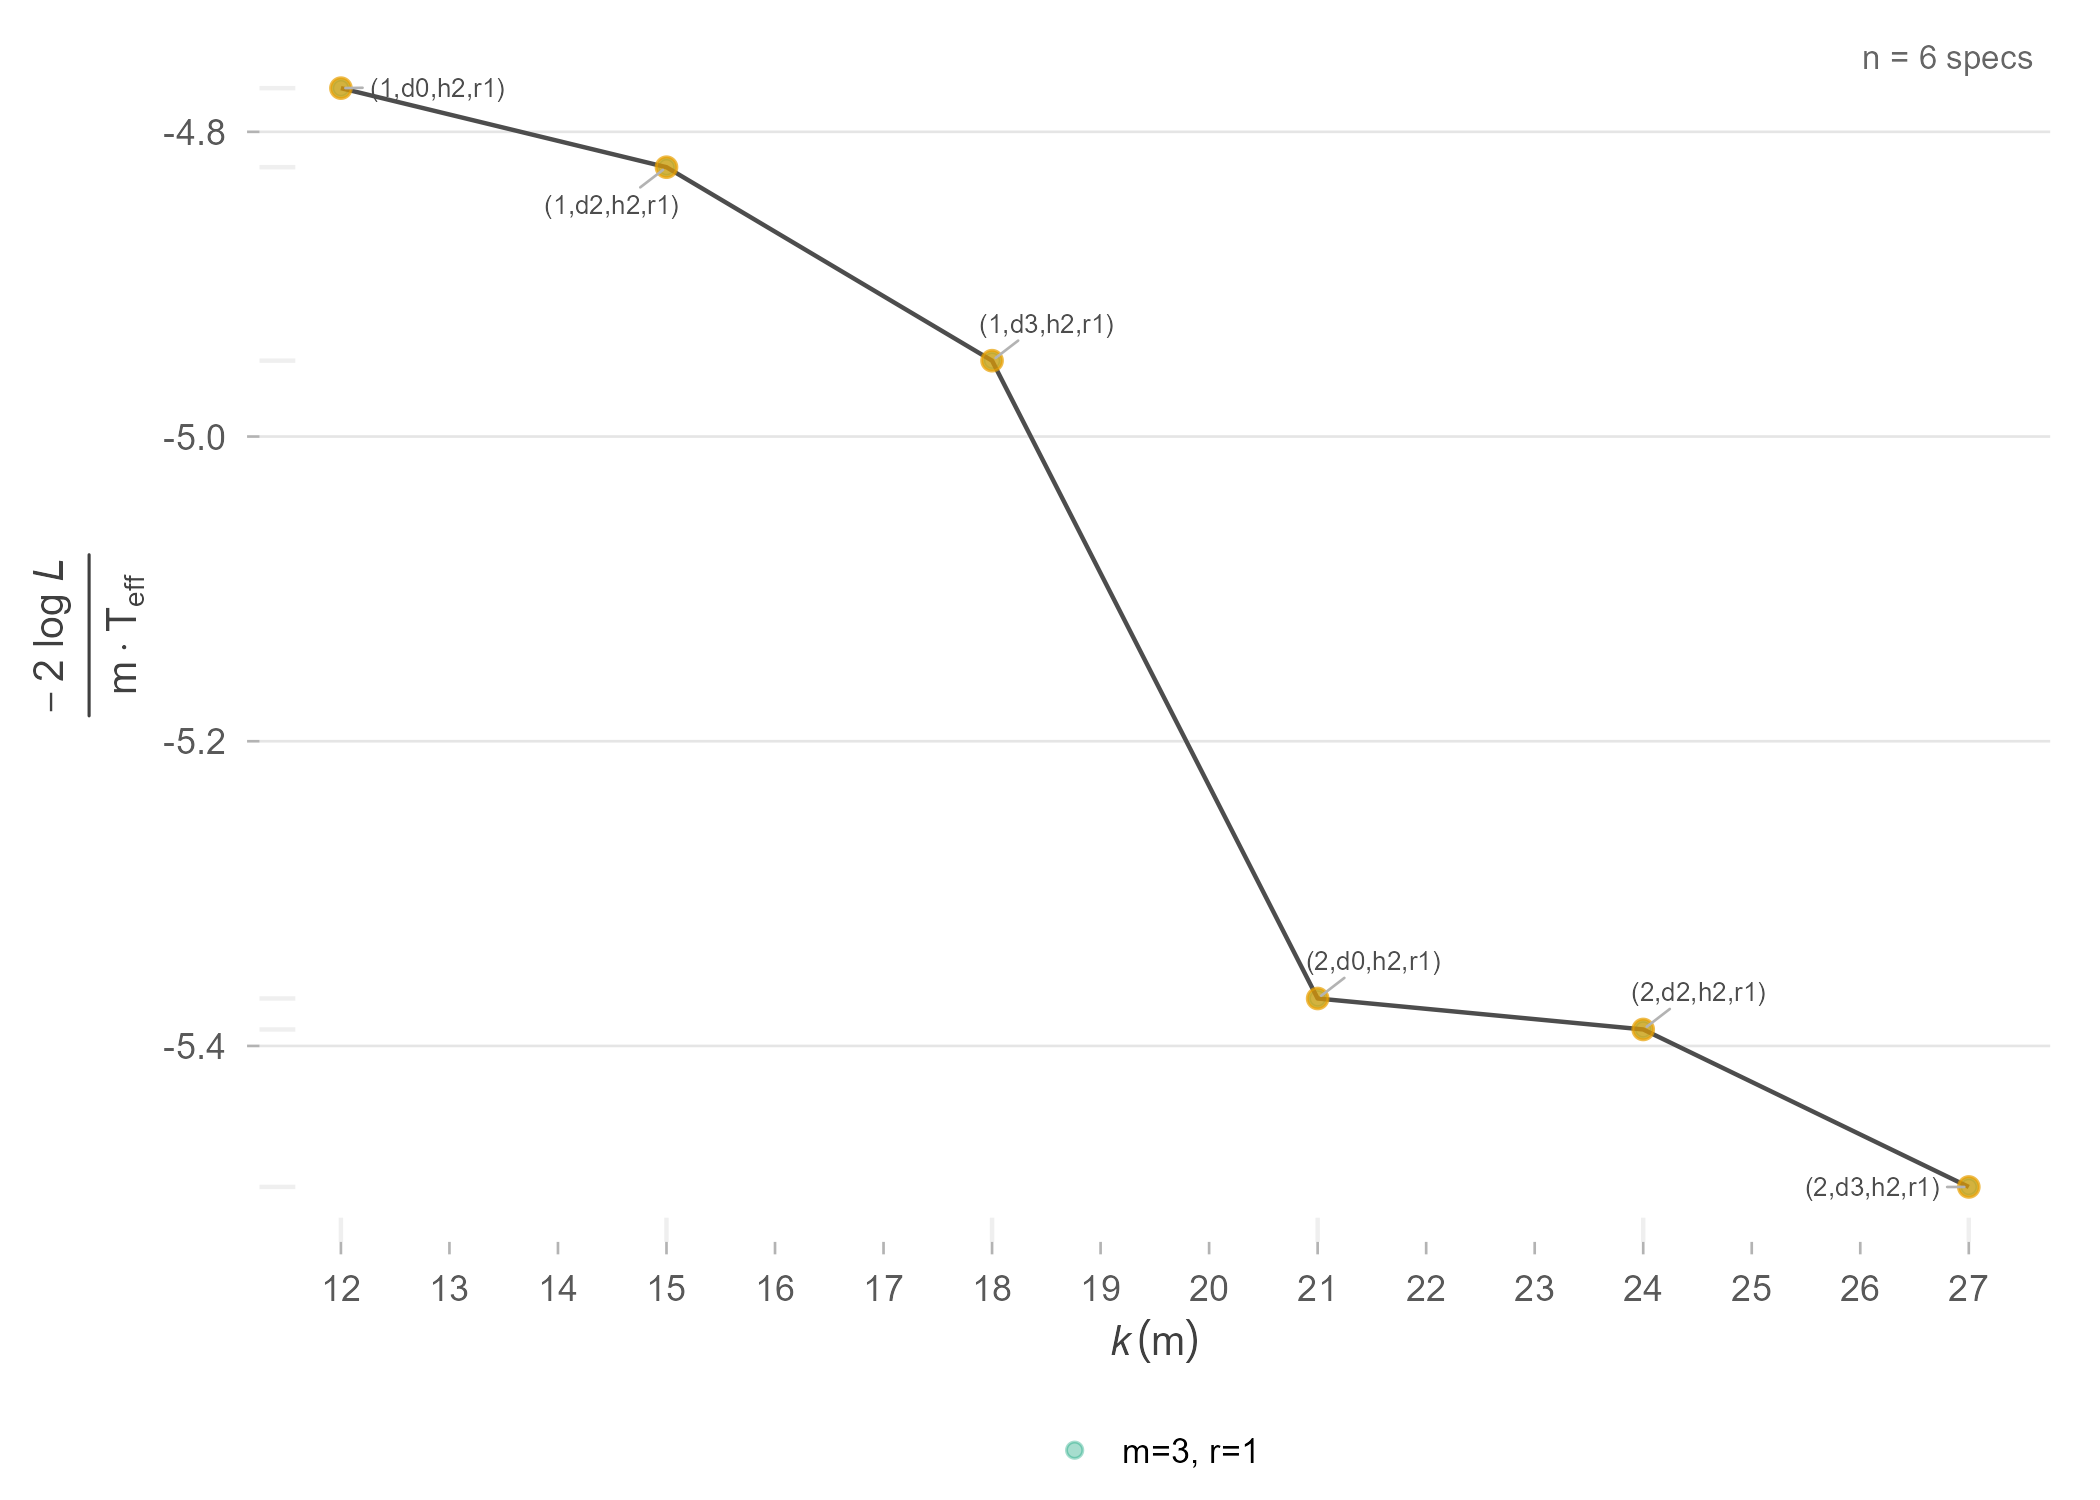
\includegraphics[width=0.86\linewidth]{figures/fig_S2_pooled_frontier.png}
\caption*{\footnotesize Source: Author's elaboration.}
\end{figure}

Figure~\ref{fig:s2-focal-cu-exploitation-diptych} plots the constructed rate of capacity utilization alongside the rate of exploitation. In the United States, the rate of exploitation peaked in the mid-1960s, declined during the stagflation of the 1970s, and rose steadily from 1983 to 2011 as wage growth lagged behind productivity. This trajectory reveals a structural link between capacity utilization and the functional distribution of income.

\begin{figure}[H]
\centering
\caption{S2 Focal Utilization and Exploitation Diptych}
\label{fig:s2-focal-cu-exploitation-diptych}
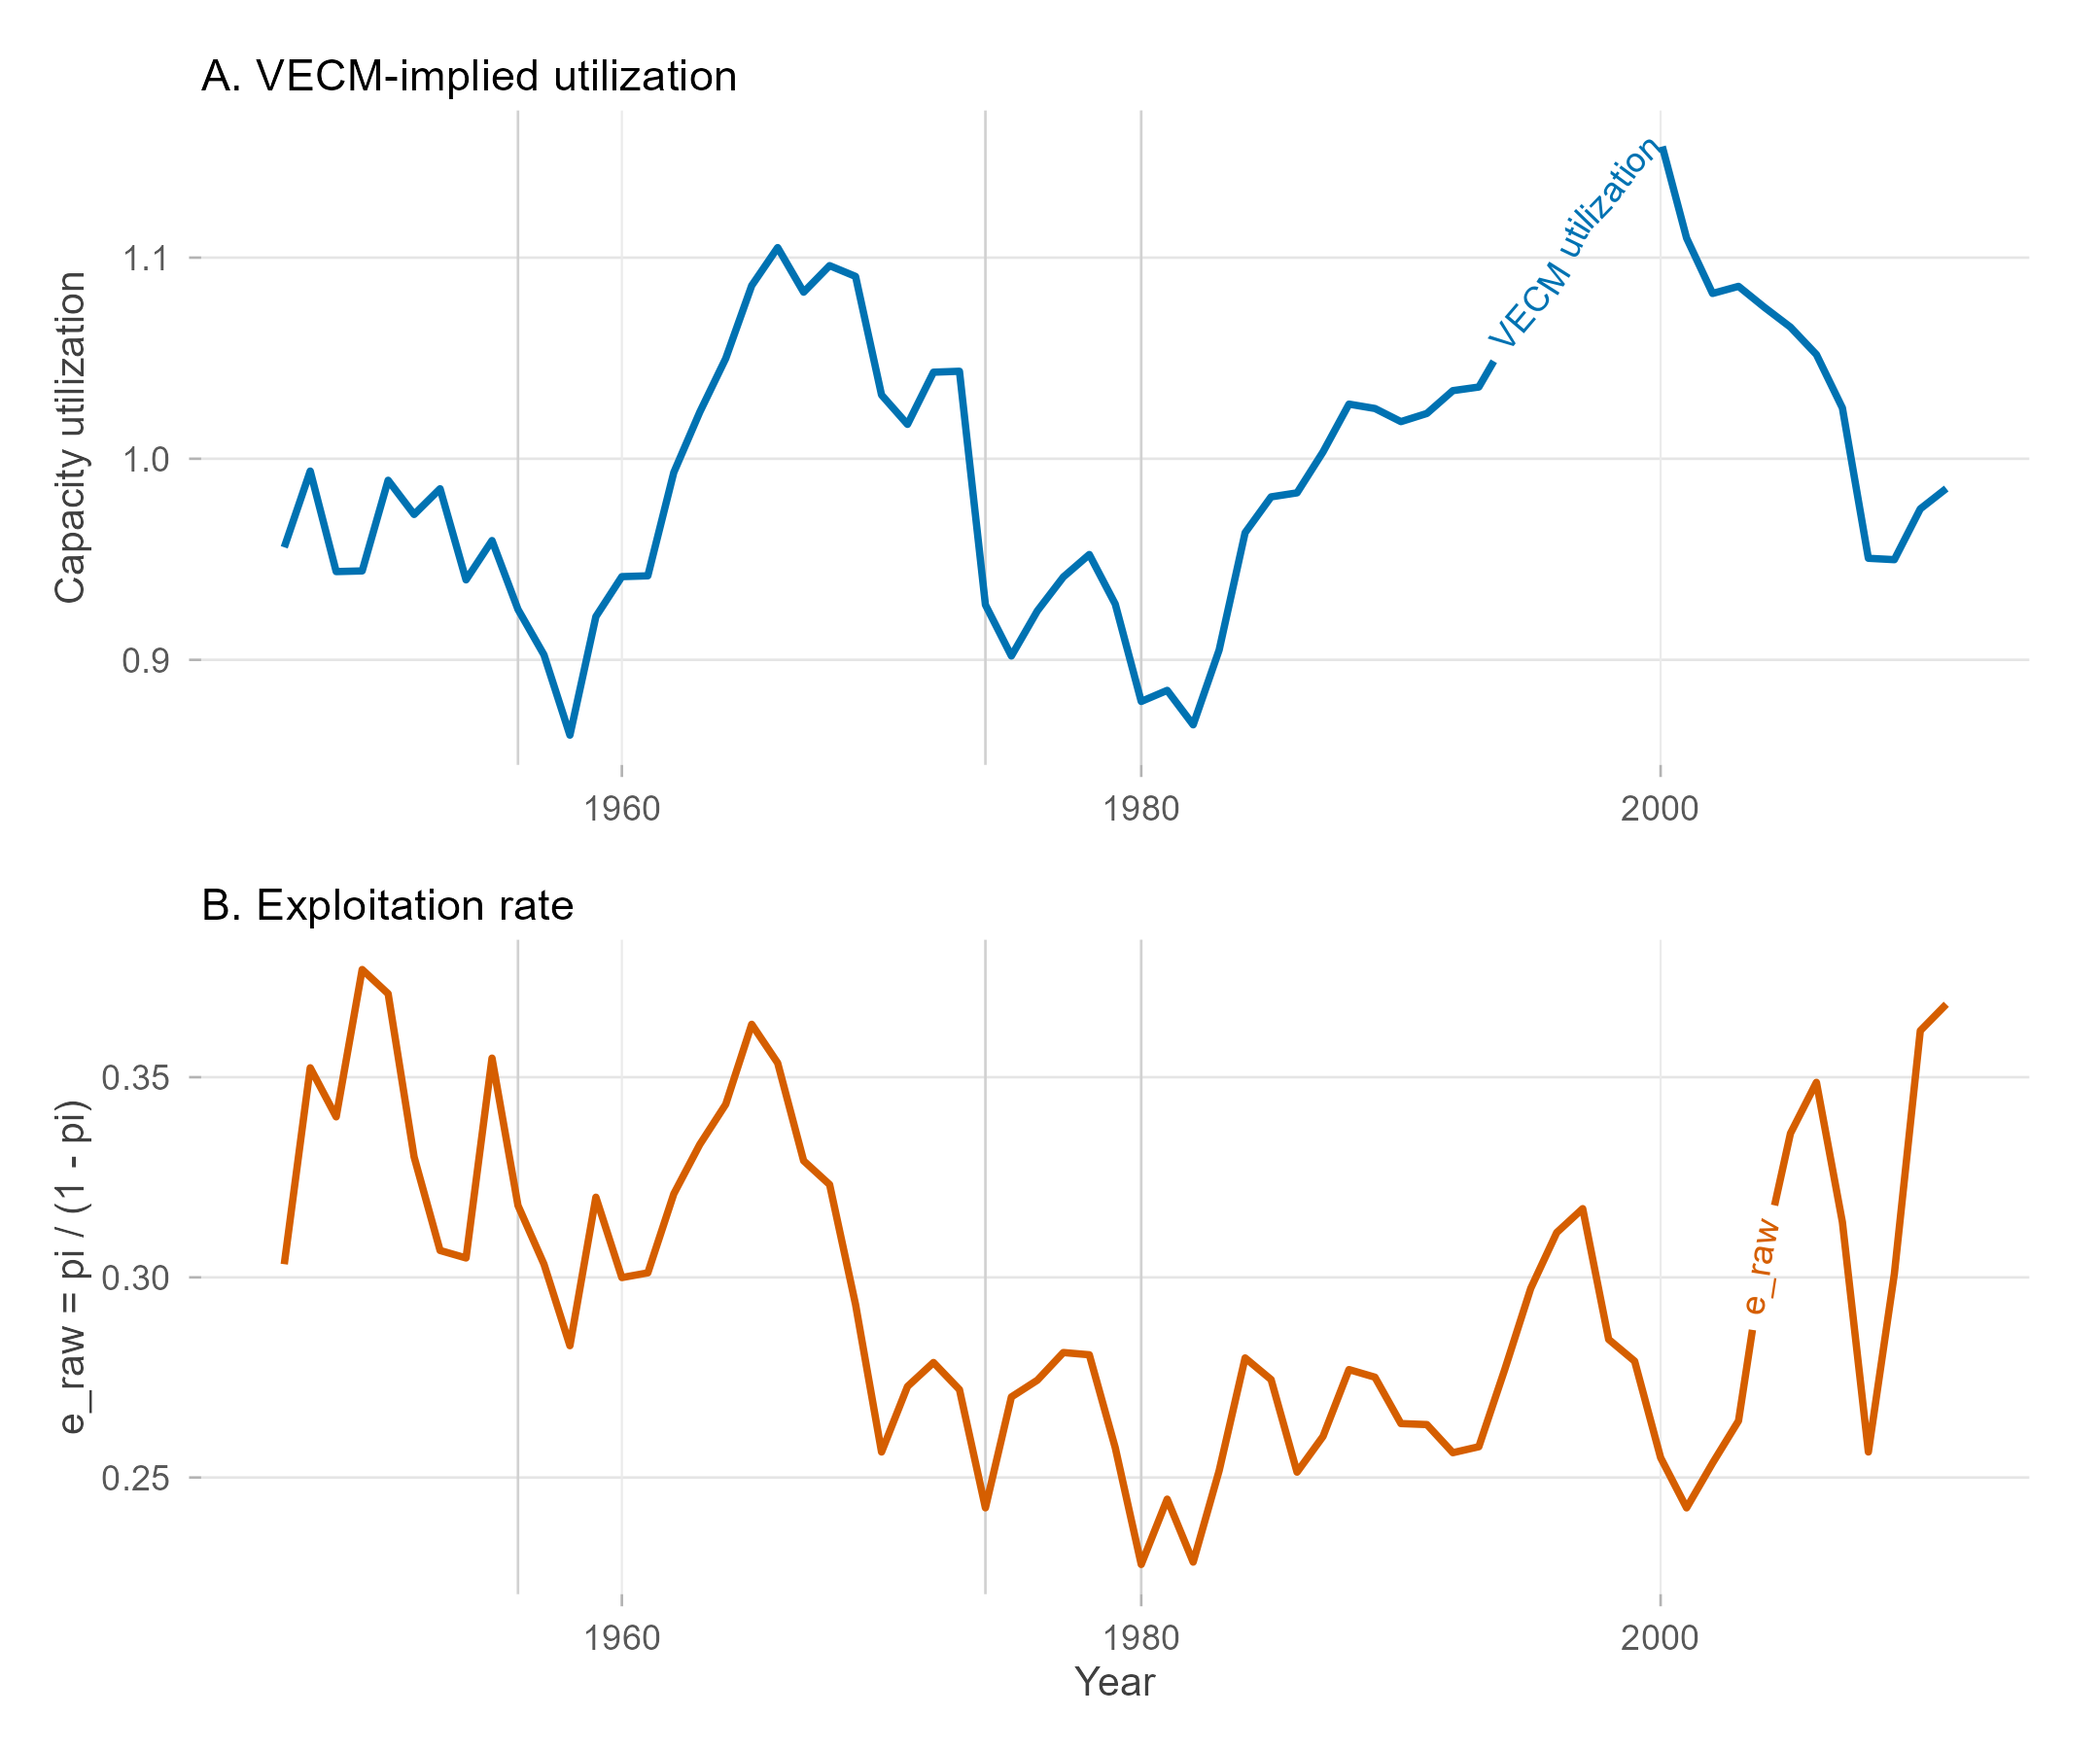
\includegraphics[width=0.92\linewidth]{figures/fig_S2_focal_cu_exploitation_diptych.png}
\caption*{\footnotesize Source: Author's elaboration.}
\end{figure}

The theoretical rationale for including $\ln e_t$ in the cointegrating vector draws upon the classical choice-of-technique framework formalized by \citet{Kurz1986}. In capitalist economies, converting capital stock into productive capacity is not an invariant technical relationship. Cost-minimizing firms select techniques from an available technology set based on prevailing wage rates and profit margins. Changes in distribution shift relative factor costs, prompting firms to adjust techniques, machine speeds, and shift arrangements. When distribution is omitted from the state vector, these technical adjustments appear as persistent residual drift in the output--capital ratio, causing bivariate cointegration tests to fail. Including $\ln e_t$ controls for technique choice, allowing the long-run relation to be identified.

Crucially, this empirical result must be distinguished from its conceptual interpretation. The VECM does not estimate ``class struggle'' or ``institutional settlement'' as direct causal parameters. Rather, institutional settlements represent the conceptual framework that explains why the output--capital relation is distributionally conditioned. In capitalist economies, productive capacity is not an insulated engineering constant, but a macro-structural outcome mediated by the institutional arrangements that govern the wage share, work intensity, and the extraction of surplus value.

\subsection{Cross-Stage Econometric Synthesis}
\label{subsec:cross_stage_synthesis_design_new}

The three-stage replication defines the strict historical and institutional boundary conditions of Shaikh’s capacity measurement strategy. While the baseline single-equation coefficient is numerically reproducible (Stage S0), it remains structurally non-unique and highly sensitive to information-criterion choices (Stage S1). Most critically, the standalone output-capital relation fails system-level cointegration, surviving within a trivariate VECM conditioned on income distribution and historical step controls (Stage S2). The long-run conversion of capital to capacity is therefore not a fixed engineering multiplier. It is an institutional reality, fundamentally shaped by systemic crises and the ongoing balance of power between wages and profits.

\begin{table}[H]
\centering
\caption{Cross-Stage Synthesis of the Cointegration Architecture}
\label{tab:cross_stage_synthesis}
\small
\begin{tabular}{@{}>{\raggedright\arraybackslash}p{3.2cm}>{\raggedright\arraybackslash}p{4.6cm}>{\raggedright\arraybackslash}p{5.6cm}@{}}
\toprule
Stage & Outcome & Interpretive Bound \\
\midrule
\midrule
S0 & Approximate single-equation reproducibility & Shaikh's method is reproducible, but not exactly \\
S1 & Non-empty admissible ARDL grid; non-unique retained benchmark & Model selection is driven by information-criterion choice \\
S2 Bivariate & 48 attempted, 36 estimated, 0 admissible & Output--capital system is not self-sufficient over 1947--2011 (12 admissible over 1947--2007) \\
S2 Trivariate Rank One & 48 attempted, 36 estimated, 6 admissible & Restricted survival with logged exploitation and $h_2$ step controls \\
S2 Trivariate Rank Two & 48 attempted, 36 estimated, 0 admissible & No retained dual-vector system \\
\bottomrule
\end{tabular}
\caption*{\footnotesize Source: Author's elaboration.}
\end{table}

A key result of my system-level estimation is that the bivariate VECM yields zero admissible specifications over the full post-war period (1947--2011, $T=65$). Across the 48 attempted bivariate specifications (36 successfully estimated) evaluated over alternative lag lengths and deterministic trends, the Johansen trace test fails to reject the null hypothesis of no cointegration ($r=0$) at the 5\% level.

Re-estimating the grid over Shaikh's pre-crisis sample period (1947--2007, $T=61$) shows that this bivariate failure reflects sample sensitivity. Over the pre-2008 sample, the bivariate system yields 12 admissible specifications (out of 36 estimated), producing an estimated elasticity of $\hat{\theta} \in [0.88, 0.91]$. Adding the four years of the Great Recession (2008--2011) disrupts this relation: the sharp fall in value added relative to a slow-depreciating capital stock introduces persistent drift into the residuals, causing bivariate cointegration to break down. I report both sample outcomes to clarify this sensitivity: single-equation models that report cointegration over the full sample without testing system rank miss this post-2007 divergence.

In contrast to the bivariate models, the trivariate system including the logged exploitation rate ($\ln e_t$) identifies cointegration over the full 1947--2011 period, producing six admissible specifications at rank $r=1$ (out of 36 estimated). All six surviving specifications include step controls for 1956, 1974, and 1980 ($S_{1956}, S_{1974}, S_{1980}$, denoted $h_2$). Estimating the specification without step controls ($h_0$) yields zero admissible models across all lag orders. This shows that identifying a cointegrating relationship requires controlling for major institutional shocks: the post-Korean War downturn, the 1974 oil and profitability crisis, and the 1980 Volcker monetary tightening.

\section{Discussion}
\label{sec:discussion}

The empirical findings across Stages S0, S1, and S2 demonstrate that the aggregate output--capital relation does not constitute an insulated engineering benchmark. Cointegration fails entirely in the standalone bivariate system over the post-war period, and within the tested full-sample system grid, long-run stability becomes recoverable only when the rate of exploitation enters the state vector alongside historical step controls. This empirical contrast motivates the central conceptual interpretation of this paper: productive capacity is an institutionally conditioned outcome of capitalist accumulation.

Crucially, ``institutional settlement'' must be understood as an analytical interpretation of the econometric results rather than an estimated parameter. The VECM does not directly measure class struggle or institutional power. Instead, the institutional settlement framework explains why the bivariate relation fails in isolation and why distribution enters the cointegrating space with such dominant statistical precision ($\hat{\beta}_e = 20.02, t = 7.90$, compared to the imprecisely identified capital elasticity $\hat{\theta} = 0.73, \text{SE} = 4.85$). In capitalist economies, the conversion of a given stock of physical equipment into potential output is not governed solely by technical engineering coefficients. It depends on the organization of the labor process, machine speeds, shift patterns, and managerial authority on the shop floor. These conditions are mediated by the historical compromises and power balances between capital and labor that determine the functional distribution of income. When distribution is omitted, the tested bivariate systems exhibit persistent drift in the output--capital relation. The recovery of cointegration in specifications including $\ln e_t$ is consistent with distributionally mediated adjustments in technique and work organization, but the VECM does not identify that mechanism causally.

While Stage S1 provides the primary statistical evidence for sub-unitary elasticities across retained no-trend specifications in the bounds-passing ARDL grid ($\hat{\theta} \in [0.65, 0.95]$), the focal point estimate in Stage S2 ($\hat{\theta} \approx 0.73$) also sits within the structural overaccumulation interval ($\theta < 1.0$), albeit with wide normalized estimation uncertainty. If interpreted through this point estimate, the profit rate decomposition,
\begin{equation}
r_t \equiv \frac{\Pi_t}{K_t} = \left(\frac{\Pi_t}{Y_t}\right) \left(\frac{Y_t}{Y^p_t}\right) \left(\frac{Y^p_t}{K_t}\right) = \pi_t \, \mu_t \, \left(\frac{Y^p_t}{K_t}\right),
\end{equation}
carries significant implications for classical and Marxian crisis theory. The maximum potential profit rate is governed by the capital-capacity ratio $Y^p_t / K_t$. When $\theta = 1.0$, capital accumulation expands capacity proportionally, preserving the capacity-capital ratio in the absence of technical change. When $\theta < 1.0$, however, the corporate sector operates under conditions of structural overaccumulation: capital equipment accumulates faster than potential output expands, placing downward pressure on $Y^p_t / K_t$ and, conditional on distribution, on potential profitability. A higher profit share ($\pi_t$) can partly offset this pressure in the realized profit rate, whereas utilization below normal capacity ($\mu_t < 1$) further depresses realized profitability.

The dynamic adjustment structure of the focal VECM also speaks to the long-standing debate between Sraffian and Neo-Kaleckian macroeconomics. In the focal system, the estimated error-correction loading for capital is statistically indistinguishable from zero ($\hat{\alpha}_k = 0.0003, t=0.92$), while the primary burden of error correction falls on the rate of exploitation ($\hat{\alpha}_e = -0.019, t=-4.25$). The absence of statistically detectable error-correction adjustment in capital accumulation is suggestively aligned with classical-Sraffian models in which long-run investment is autonomous, rather than with Neo-Kaleckian models where investment responds endogenously to capacity utilization gaps. Nevertheless, this point-estimate asymmetry should not be overstated as a definitive statistical refutation of Neo-Kaleckian closure without a joint likelihood-ratio restriction test. Moreover, insofar as sub-unitary elasticity estimates ($\hat{\theta} < 1.0$) decouple capacity from capital, the long-run dynamics of accumulation cannot be evaluated under the balanced-growth knife-edge assumption that both traditions routinely share.

Several methodological boundaries qualify these findings. First, the empirical analysis relies on single-sector corporate data, abstracting from inter-sectoral transfers, department-level disproportionalities, and uneven development across branches of production. Second, the transformation elasticity $\theta$ is estimated as a fixed parameter over the 1947--2011 period, averaging across distinct institutional regimes (such as the post-war Golden Age and the neoliberal transition). Third, the bivariate failure reflects sample sensitivity: while bivariate systems yield admissible cointegrating relations over the 1947--2007 sub-sample, cointegration is lost over the full 1947--2011 sample, coinciding with the acute contraction of the Great Recession where value added dropped sharply relative to the corporate capital stock.

\section{Conclusion}
\label{sec:conclusion}

This paper critically evaluated Anwar Shaikh's (2016) capacity utilization measure, investigating whether the underlying aggregate output--capital relation provides a stable technical benchmark for macroeconomic analysis. Re-examining this relation through an econometric replication across three stages yields three core findings that establish the evidentiary ordering of the paper.

First, at the single-equation level (Stage S0), Shaikh's baseline ARDL(2,4) specification is approximately reproducible within canonical data bounds ($\hat{\theta} \approx 0.72$ versus Shaikh's published 0.66). Second, testing this relationship across an exhaustive lattice of 500 ARDL specifications (Stage S1) reveals disciplined non-uniqueness: the estimated transformation elasticity ranges across the informational frontier from 0.65 to 0.95 among retained no-trend specifications (reaching 2.20 in trend-containing models). The recovered capacity ceiling is sensitive to lag profiles and deterministic trend assumptions, demonstrating that single-equation models cannot identify a unique technical parameter.

Third, system-level estimation (Stage S2) demonstrates that across 48 attempted bivariate VECM specifications, 36 are successfully estimated, and none of those 36 identifies an admissible cointegrating relation over the 1947--2011 sample. Within the tested full-sample system grid, cointegration becomes recoverable only when the rate of exploitation enters the state vector alongside historical step controls. In the focal trivariate VECM, the rate of exploitation enters with dominant statistical precision ($\hat{\beta}_e = 20.02, t = 7.90$), while the transformation elasticity point estimate ($\hat{\theta} \approx 0.73$) sits within the structural overaccumulation interval ($\theta < 1.0$) alongside substantial estimation uncertainty.

The overarching conclusion is that aggregate productive capacity is not an insulated engineering constant. Rather, the output--capital relation is distributionally conditioned and socially structured. Macroeconomic models that treat the capacity ceiling as an autonomous physical limit risk obscuring the institutional arrangements and distributive conflicts that govern how productive equipment is converted into potential output in capitalist economies.


\clearpage
\begingroup
\setlength{\bibsep}{2.5pt}
\bibliographystyle{apalike}
\bibliography{references}
\endgroup

\clearpage
\begin{appendices}
\section{Derivation of Accumulation Dynamics under Unbalanced Growth}
\label{app:acc_dynamics}

This appendix provides the derivation of the dynamical equations summarized in \S\ref{subsec:balanced_unbalanced_growth} and \S\ref{subsec:trend_stabilized_closure}. All results follow from three components: the accounting identity $\hat{k} + \delta = \phi^p B$, the unbalanced growth closure $g_{Y^p} = \theta g_K$, and the investment-savings closure $\phi^p = s$.

\subsection{The Unbalanced Growth Closure: Derivation of the Bernoulli ODE}
\label{app:bernoulli}

The accounting identity under the investment-savings closure is:
\begin{equation}\label{eq:app_identity}
    \hat{k} + \delta = s \, B.
\end{equation}
Differentiating with respect to time yields:
\begin{equation}\label{eq:app_diff}
    \frac{d\hat{k}}{dt} = s \, \dot{B}.
\end{equation}
Expressing $\dot{B}$ in terms of the growth rate of capital productivity ($\hat{b}$):
\begin{equation}\label{eq:app_Bdot}
    \dot{B} = B \, \hat{b}.
\end{equation}
Substituting this into equation~\eqref{eq:app_diff} and utilizing the accounting identity $sB = \hat{k} + \delta$ results in the acceleration identity:
\begin{equation}\label{eq:app_chain}
    \frac{d\hat{k}}{dt} = (\hat{k} + \delta) \, \hat{b}.
\end{equation}
Recall that capital productivity is $B \equiv Y^p / K$, which in growth rates implies $\hat{b} = \hat{y}^p - \hat{k}$. Under the unbalanced growth closure $g_{Y^p} = \theta g_K$ (or $\hat{y}^p = \theta \hat{k}$ in growth rate notation), this gives the growth rate of capital productivity as $\hat{b} = (\theta - 1) \, \hat{k}$. Substituting this into equation~\eqref{eq:app_chain} provides the acceleration dynamic:
\begin{equation}\label{eq:app_bernoulli}
    \boxed{\frac{d\hat{k}}{dt} = (\theta - 1) \, \hat{k} \, (\hat{k} + \delta)}, \quad \text{where } \hat{k} \text{ and } \delta \text{ are expressed in consistent temporal and physical units}.
\end{equation}
This is a Bernoulli equation of order 2 in $\hat{k}$, where the nonlinearity arises from the product $\hat{k}(\hat{k} + \delta)$.

\subsection{Analytical Solution}
\label{app:solution}

Expanding equation~\eqref{eq:app_bernoulli} gives:
\begin{equation}\label{eq:app_expanded}
    \frac{d\hat{k}}{dt} = (\theta - 1)\,\hat{k}^2 + (\theta - 1)\,\delta\,\hat{k}.
\end{equation}
Applying the Bernoulli substitution $v \equiv \hat{k}^{-1}$ with $\dot{v} = -\hat{k}^{-2}\dot{\hat{k}}$ transforms the equation into a first-order linear ODE:
\begin{equation}\label{eq:app_linear_standard}
    \dot{v} + (\theta - 1)\delta\,v = -(\theta - 1).
\end{equation}
The solution for $v(t)$, given initial conditions $v_0 = \hat{k}_0^{-1}$, is:
\begin{equation}\label{eq:app_v_simplified}
    v(t) = \left(v_0 + \frac{1}{\delta}\right) e^{-(\theta-1)\delta\,t} - \frac{1}{\delta}.
\end{equation}
Inverting $v(t)$ yields the explicit path for the net accumulation rate:
\begin{equation}\label{eq:app_khat_solution}
    \boxed{\hat{k}(t) = \frac{1}{\left(\frac{1}{\hat{k}_0} + \frac{1}{\delta}\right) e^{-(\theta-1)\delta\,t} - \frac{1}{\delta}}}.
\end{equation}

\subsection{Equilibria and Stability Analysis}
\label{app:stability}

The equilibria $\hat{k}^*$ are defined by $(\theta - 1)\,\hat{k}\,(\hat{k} + \delta) = 0$. For $\theta \neq 1$, the roots are $\hat{k}_1^* = 0$ (stationary net capital) and $\hat{k}_2^* = -\delta$ (zero gross investment). Linearizing around $\hat{k}^* = 0$ via the Jacobian $f'(\hat{k}) = (\theta - 1)(2\hat{k} + \delta)$ yields:
\begin{itemize}
    \item Over-accumulation ($\theta < 1$): $f'(0) < 0$ --- the stagnation equilibrium is locally stable.
    \item Under-accumulation ($\theta > 1$): $f'(0) > 0$ --- the stagnation equilibrium is unstable.
\end{itemize}

\subsection{The Trend-Stabilized Closure: Derivation of the Quadratic ODE}
\label{app:extended_derivation}

Under the trend-stabilized closure $\hat{y}^p = \theta\hat{k} + b$, the growth rate of capital productivity is:
\begin{equation}\label{eq:app_bhat_extended}
    \hat{b} = (\theta - 1)\hat{k} + b.
\end{equation}
Substituting this into the acceleration identity (equation~\ref{eq:app_chain}) generates a quadratic ODE:
\begin{equation}\label{eq:app_extended_ode}
    \frac{d\hat{k}}{dt} = (\hat{k} + \delta)\left[(\theta - 1)\hat{k} + b\right].
\end{equation}
The equilibria are the roots of $(\hat{k} + \delta)[(\theta - 1)\hat{k} + b] = 0$:
\begin{equation}\label{eq:app_extended_roots}
    \hat{k}_1^* = -\delta, \qquad \hat{k}_2^* = \frac{b}{1 - \theta}.
\end{equation}
The Jacobian $g'(\hat{k}) = 2(\theta - 1)\hat{k} + (\theta-1)\delta + b$ evaluated at $\hat{k}_2^*$ confirms local stability for the empirically relevant case ($\theta < 1$ and $b > 0$): the interior root $b/(1-\theta)$ acts as a strictly positive attractor, preventing stagnation. As $b \to 0$, the trend-stabilized closure collapses to the unbalanced growth attractor at $\hat{k}^* = 0$.

\clearpage
% ================================================================
% APPENDIX A: DATA CONSTRUCTION AND DIAGNOSTIC SUPPORT
% Supporting material for §4.2 (Data and Measurement)
% ================================================================
\section{Data Construction and Diagnostic Support}
\label{app:data_construction}

% ---------------------------------------------------------------
% A.1 — Series Glossary
% ---------------------------------------------------------------
\subsection{Series Glossary}
\label{subsec:app_glossary}

Table~\ref{tab:app_glossary} lists the core replication variables, their sources, and transformation rules. All series derive from Shaikh's (2016) data companions via Real Economic Analysis.\footnote{Replication data and construction scripts are available at Real Economic Analysis: \url{https://www.realecon.org/data}.}

\begin{table}[!ht]
\centering
\small
\setlength{\tabcolsep}{3pt}
\renewcommand{\arraystretch}{1.15}
\caption{Replication series: symbols, sources, and transformations}
\label{tab:app_glossary}
\begin{tabular}{@{} >{\raggedright\arraybackslash}p{0.20\textwidth}
 >{\raggedright\arraybackslash}p{0.26\textwidth}
 >{\raggedright\arraybackslash}p{0.28\textwidth}
 >{\raggedright\arraybackslash}p{0.18\textwidth}@{}}
\hline
Symbol / Code  & Variable  & Source (table, line)  & Transformation \\
\hline
$\text{GVAcorp}_t$
 & Corporate gross value added (corrected)
 & NIPA 1.14 (L1) + imputed-interest adj.\ (Table~7.11)
 & nominal \\[3pt]
$\text{KGCcorp}_t$
 & Corporate gross capital stock (GPIM-adjusted)
 & Fixed Asset 6.1 (L9); IRS Statistics of Income; GPIM recursion
 & nominal \\[3pt]
$\text{KNCcorp}_t$
 & Corporate net capital stock (GPIM-adjusted)
 & same as above
 & nominal \\[3pt]
$\text{KNCcorpbea}_t$
 & Corporate net capital stock (BEA 2011 official)
 & Fixed Asset 6.1 (L9)
 & nominal \\[3pt]
$p_t$
 & Common deflator
 & $pKN$ index, 2005=100
 & (KNCcorp/KNRcorp)*100 \\[3pt]
$y_t$
 & Real log output
 & constructed
 & $\ln(\text{VAcorp}_t/p_t)$ \\[3pt]
$k_t$
 & Real log capital
 & constructed
 & $\ln(\text{KGCcorp}_t/p_t)$ \\[3pt]
$\text{Profshcorp}_t$
 & Corporate profit share (corrected)
 & NIPA 1.14 (L8, L1$-$L2) + imputed-interest adj.
 & ratio \\
\hline
\end{tabular}
\par\vspace{0.4em}
\footnotesize\textit{Note:} All BEA and NIPA data downloaded in the replication vintage. Shaikh's original series used data downloaded in 2011 \citep[Appendix~6.7, fn.~1]{Shaikh2016}; discrepancies attributable to subsequent BEA revisions are possible and noted where material.
\par\vspace{0.2em}
\footnotesize \textit{Source:} \href{https://www.realecon.org/data}{Real Economic Analysis Data Tables}
\end{table}

% ---------------------------------------------------------------
% A.2 — Imputed-Interest Correction
% ---------------------------------------------------------------
\subsection{Imputed-Interest Correction}
\label{subsec:app_impint}

The NIPA corporate value added figure includes imputed financial intermediation services as a cost to non-financial corporations. The corporate imputed-interest adjustment removes this component:
%
\begin{equation}
\label{eq:app_impint}
\text{CorpImpIntAdj}_t \equiv -\text{BankMonIntPaid}_t - \text{CorpNFNetImpIntPaid}_t,
\end{equation}
%
where $\text{BankMonIntPaid}_t$ is NIPA Table~7.11 (lines 4+44+73 minus lines 28+52+91) and $\text{CorpNFNetImpIntPaid}_t$ is NIPA Table~7.11 (line~74 minus line~53). In 2009 the adjustment raises corporate net operating surplus by approximately 10\,\%. Figure~\ref{fig:app_impint_impact} displays the corrected versus uncorrected series and their ratio.

\begin{figure}[!ht]
\centering
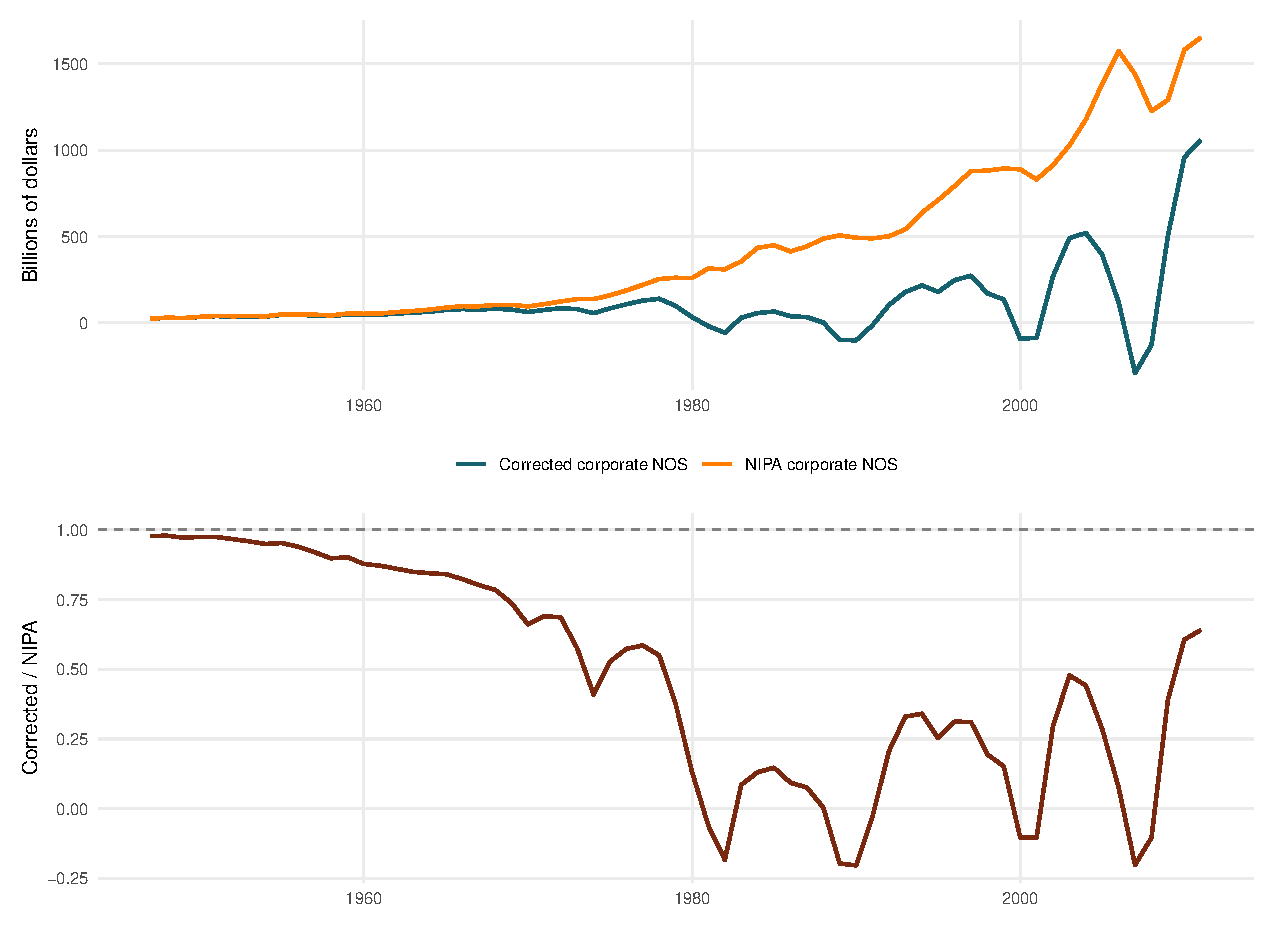
\includegraphics[width=0.85\textwidth]{appendixA/figures/fig_A9_imputed_interest_adjustment.pdf}
\caption{Imputed interest adjustment impact: corrected corporate NOS versus NIPA corporate NOS (1947--2011). Ratio shows magnitude of adjustment.}
\label{fig:app_impint_impact}
\end{figure}

% ---------------------------------------------------------------
% A.3 — Corporate Output: GVAcorp
% ---------------------------------------------------------------
\subsection{Corrected Corporate Output: \texorpdfstring{$\text{GVAcorp}_t$}{GVAcorp}}
\label{subsec:app_gva}

\begin{equation}
\label{eq:app_gva}
\text{GVAcorp}_t \equiv \text{GVAcorpnipa}_t + \text{CorpImpIntAdj}_t,
\end{equation}
%
where $\text{GVAcorpnipa}_t$ is NIPA Table~1.14 (line~1) and $\text{CorpImpIntAdj}_t$ is defined in equation~\eqref{eq:app_impint}.

% ---------------------------------------------------------------
% A.4 — Corporate Capital Stock: KGCcorp (GPIM)
% ---------------------------------------------------------------
\subsection{Reconstructed Corporate Capital Stock: \texorpdfstring{$\text{KGCcorp}_t$}{KGCcorp}}
\label{subsec:app_gpim}

\paragraph{GPIM accumulation rule.}
The current-cost capital stock is accumulated as:
%
\begin{equation}
\label{eq:app_gpim}
K_t = IG_t + z_t^* \cdot K_{t-1},
\qquad
z_t^* \equiv (1 - z_t)\frac{p^K_t}{p^K_{t-1}},
\end{equation}
%
where $IG_t$ is nominal gross investment, $z_t$ is the period depreciation rate, and $z_t^*$ is the survival-and-revaluation factor that reflates the surviving stock to current replacement cost.

\paragraph{Three adjustments (applied before the recursion).}
\begin{enumerate}
\item \textbf{Depletion rates.} BEA 1993 finite service lives replace the BEA 2011 infinite-lives assumption, implying higher depreciation and lower retirement rates consistent with physical exhaustion.
\item \textbf{Initial values.} BEA 1993 initial values anchored to 1925 replace the BEA 2011 starting values. The 1993 values are lower, producing faster accumulation growth and convergence to the official path by approximately 1977.
\item \textbf{Great Depression correction.} The IRS corporate book value index \citep[Series~V~115, pp.~924--926]{UScensus1975} is applied over 1925--1947, rescaling the BEA historical stock by the IRS/BEA ratio each year. The GPIM recursion resumes from 1947. Net effect: $\text{KNCcorp}_t$ is approximately 28\,\% lower in 1947 than the BEA 2011 official measure.
\end{enumerate}

\paragraph{Inventories.}
IRS corporate balance sheet inventory ratios are extrapolated over 1947--1989 via a linear fit to the 1990--2011 IRS/BEA ratio, rescaled to the adjusted GPIM stocks, and added to $\text{KGCcorp}_t$. Source: IRS Statistics of Income 1926--2011; FRB Flow of Funds FL105015205.A for non-financial corporate inventories in current cost.

\paragraph{Accuracy.}
The average ratio of the GPIM approximation to the BEA current-cost stock over 1947--2005 is 99.60\,\%.

\begin{figure}[!ht]
\centering
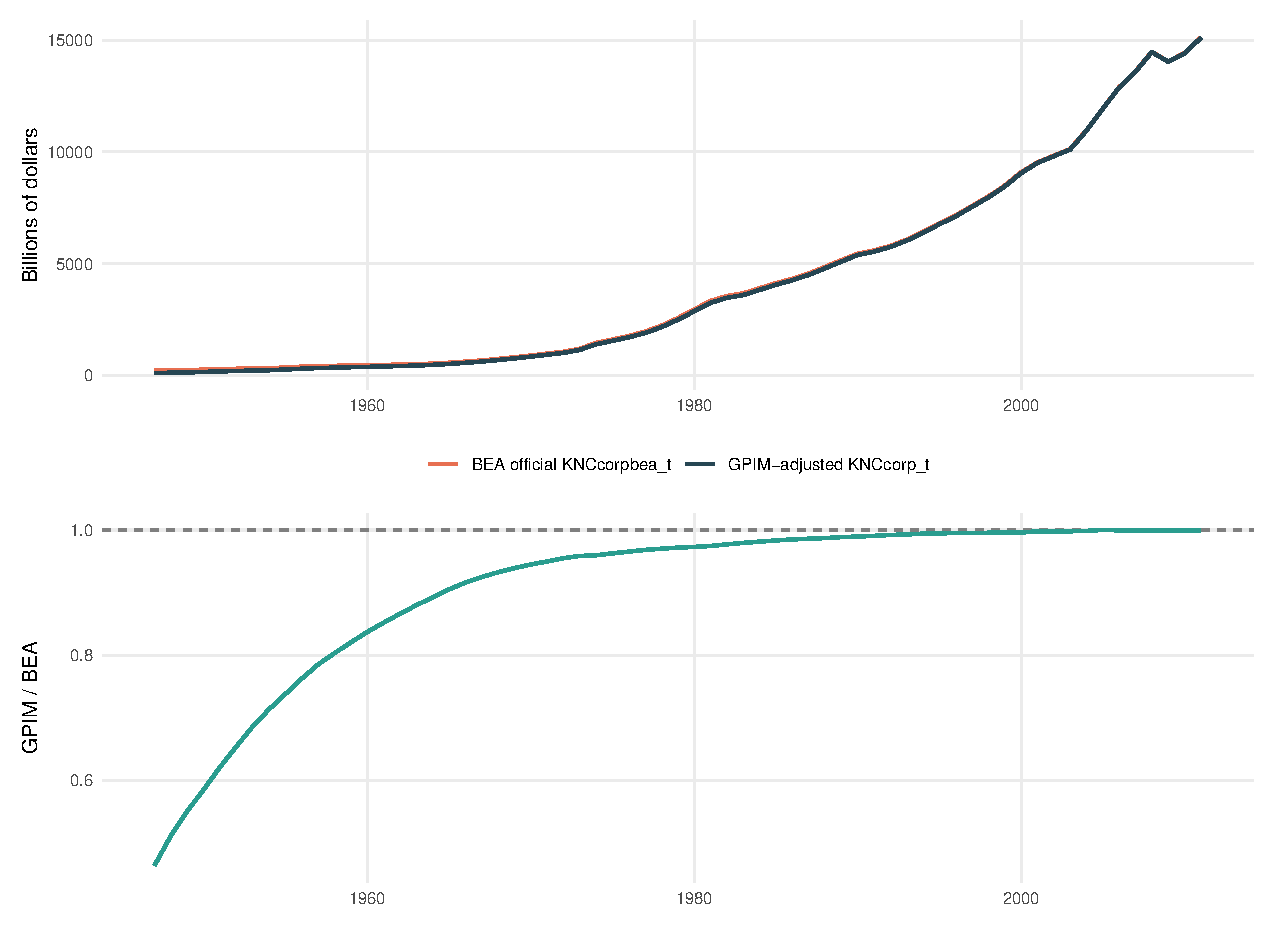
\includegraphics[width=0.85\textwidth]{appendixA/figures/fig_A6_gpim_vs_bea_capital.pdf}
\caption{GPIM-adjusted net capital stock versus BEA 2011 official series (1947--2011). Ratio plot shows convergence by ~1977.}
\label{fig:app_gpim_vs_bea}
\end{figure}

\begin{figure}[!ht]
\centering
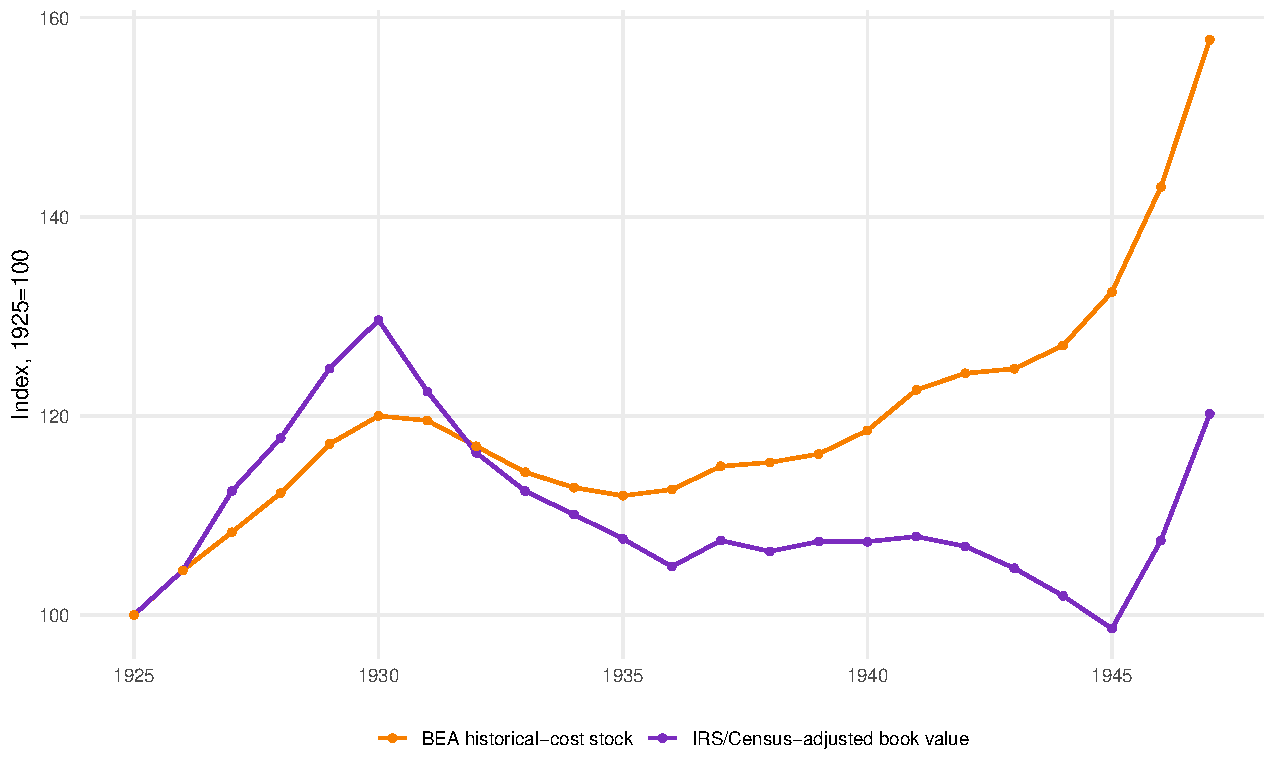
\includegraphics[width=0.85\textwidth]{appendixA/figures/fig_A7_irs_vs_bea_historical_stock.pdf}
\caption{IRS corporate book value index versus BEA historical stock (1925--1947). Both indexed to 100 in 1925.}
\label{fig:app_irs_bea_historical}
\end{figure}

\begin{figure}[!ht]
\centering
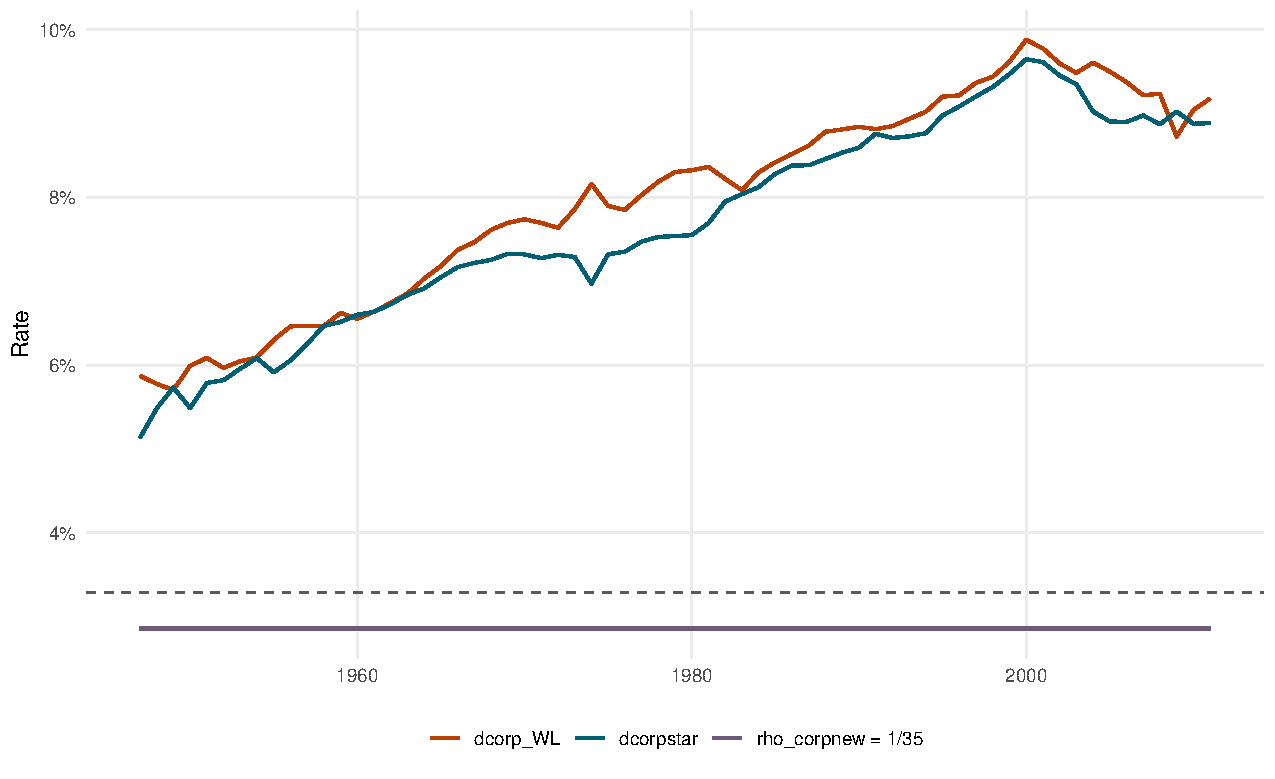
\includegraphics[width=0.85\textwidth]{appendixA/figures/fig_A8_depreciation_retirement_rates.pdf}
\caption{Depreciation and retirement rates under BEA 1993 finite service lives. The solid horizontal line indicates the corporate retirement rate ($\rho_{\text{corp}} = 1/35 \approx 2.86\%$), while the dashed horizontal line marks the critical depletion threshold ($z^* \approx 3.29\%$).}
\label{fig:app_depr_ret_rates}
\end{figure}

% ---------------------------------------------------------------
% A.5 — Common Deflator
% ---------------------------------------------------------------
\subsection{Common Deflator: \texorpdfstring{$p_t$}{p_t}}
\label{subsec:app_deflator}

The replication uses the $pKN$ implicit price deflator based at $100 = 2005$, estimated under GPIM rules. Current BEA releases employ quality-adjusted chain weights that adjust for quality vintage, breaking stock-flow consistency for accumulation accounting. The $pKN$ index preserves stock-flow consistency, ensuring the output--capital relation reflects real productive dynamics rather than quality-adjustment artifacts \citep[Appendix~6.6, Sec.~II]{Shaikh2016}.

\begin{figure}[!ht]
\centering
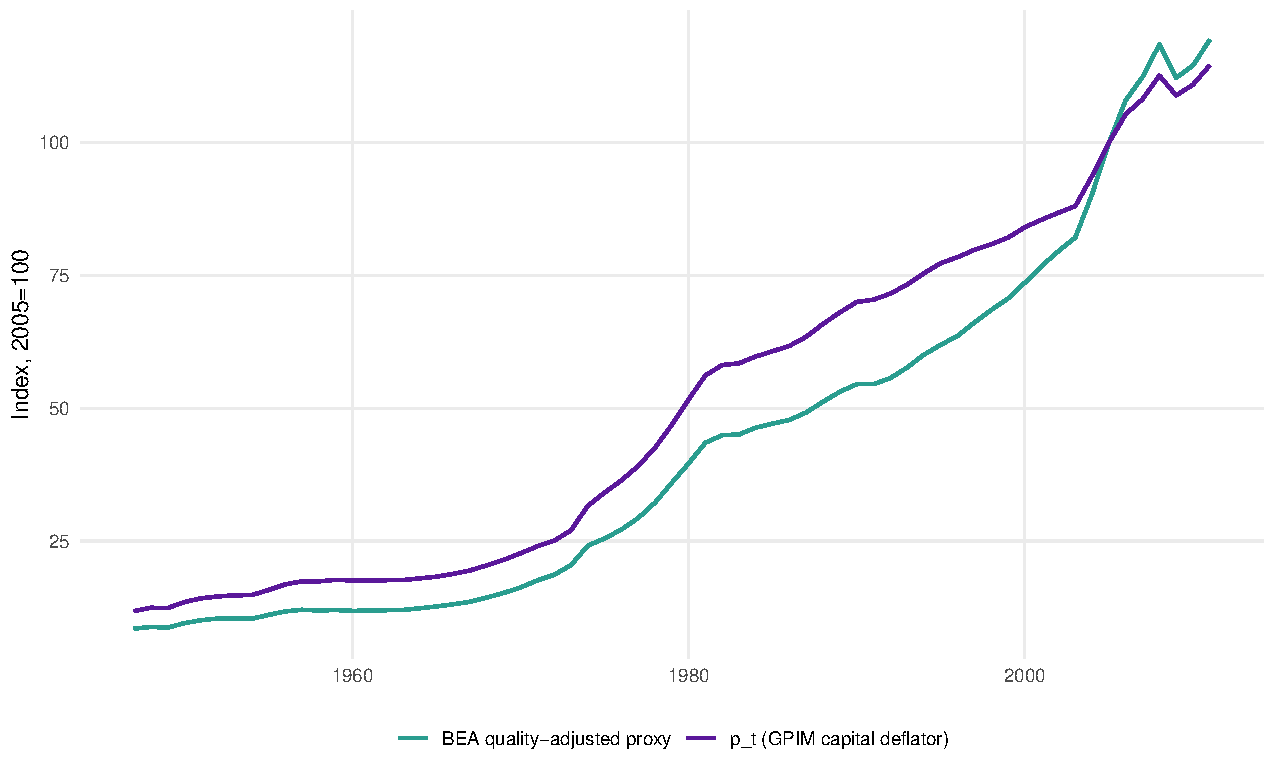
\includegraphics[width=0.85\textwidth]{appendixA/figures/fig_A4_common_deflator.pdf}
\caption{Common deflator index: GPIM-consistent $pKN$ versus BEA quality-adjusted proxy (2005=100).}
\label{fig:app_deflator_comparison}
\end{figure}

% ---------------------------------------------------------------
% A.6 — Corrected Corporate Profit Share: Profshcorp
% ---------------------------------------------------------------
\subsection{Corrected Corporate Profit Share: \texorpdfstring{$\text{Profshcorp}_t$}{Profshcorp}}
\label{subsec:app_profsh}

The same imputed-interest adjustment applied to $\text{GVAcorp}_t$ is applied to both the numerator and denominator of the profit share:
%
\begin{align}
\text{NOScorp}_t &\equiv \text{NOScorpnipa}_t + \text{CorpImpIntAdj}_t, \label{eq:app_nos} \\
\text{VAcorp}_t &\equiv \text{VAcorpnipa}_t + \text{CorpImpIntAdj}_t, \label{eq:app_va} \\
\text{Profshcorp}_t &\equiv \frac{\text{NOScorp}_t}{\text{VAcorp}_t}, \label{eq:app_profshcorp}
\end{align}
%
where $\text{NOScorpnipa}_t$ is NIPA Table~1.14 (line~8) and $\text{VAcorpnipa}_t$ is NIPA Table~1.14 (line~1 minus line~2).

% ---------------------------------------------------------------
% A.7 — Descriptive Statistics and Unit Root Tests
% ---------------------------------------------------------------
\subsection{Descriptive Statistics and Unit Root Tests}
\label{subsec:app_desc_stats}

Table~\ref{tab:app_summary_stats} reports summary statistics for the core series. Table~\ref{tab:app_unit_roots} presents unit root and stationarity test results for $y_t$ and $k_t$ in levels and differences. For output, first differences ($\Delta y_t$) strongly reject the unit-root null across both ADF and PP tests ($p < 0.01$). For corporate capital accumulation, the diagnostic pattern requires more nuanced evaluation. In first differences, baseline ADF ($t = -2.067, p = 0.228$) and PP ($t = -1.903, p = 0.297$) tests on $\Delta k_t$ fail to reject a unit root at conventional levels. Furthermore, a bounded Zivot--Andrews test allowing for an endogenous break in intercept (Model~A) yields an estimated break year of 1963 with a test statistic of $-3.7469$, which fails to reject the unit-root null against the 5\% critical value of $-4.80$ in this short annual sample. However, complementary high-power and stationarity diagnostics provide positive support for differenced stationarity: the Elliott--Rothenberg--Stock (ERS) point-optimal test yields $P_T = 2.4029$, which rejects the unit-root null at the 5\% critical value ($3.11$); the KPSS test yields $\text{LM} = 0.2828$, which fails to reject stationarity of $\Delta k_t$ at the 10\% level ($0.347$), a result that is robust across autocorrelation-adjusted bandwidths; and the characteristic roots of an AIC-selected AR(3) model for $\Delta k_t$ lie strictly in the stationary region (minimum root modulus $1.2631$, dominant companion eigenvalue $\lambda_1 = 0.7917$). In second differences, $\Delta^2 k_t$ rejects the unit-root null ($t = -4.2835$). Taken jointly, the complementary tests support treating $k_t$ as $I(1)$, although capital-stock growth is highly persistent in this short annual sample. Methodologically, Pesaran--Shin--Smith bounds inference accommodates regressors that are $I(0)$ or $I(1)$, but not $I(2)$; these diagnostics therefore remove the specific concern that capital stock may fall outside the admissible $I(0)/I(1)$ range. For system-level estimation, the complementary diagnostics support treating $k_t$ as $I(1)$, which is consistent with the maintained integration-order treatment of the system variables in the VECM.

% ---------------------------------------------------------------
% Table A.1: Core Series Summary Statistics
% ---------------------------------------------------------------
\begin{longtable}[t]{lrrrrrrrr}
\caption{Core series summary statistics (1947--2011)}\label{tab:app_summary_stats}\\
\toprule
Variable & $N$ & Mean & Median & Std Dev & Min & Max & Skewness & Kurtosis \\
\midrule
$y_t$ & 65 & 14.9281 & 14.8653 & 0.5674 & 13.8866 & 15.7628 & $-0.1438$ & 1.8398 \\
$k_t$ & 65 & 15.9658 & 15.9810 & 0.7313 & 14.7979 & 17.1127 & $-0.0206$ & 1.6872 \\
$\Delta y_t$ & 64 & 0.0293 & 0.0355 & 0.0391 & $-0.0979$ & 0.1055 & $-0.6331$ & 3.4760 \\
$\Delta k_t$ & 64 & 0.0362 & 0.0361 & 0.0078 & 0.0186 & 0.0530 & $-0.1127$ & 2.4022 \\
$p_t$ & 65 & 50.3486 & 46.8900 & 32.8159 & 11.8262 & 114.5539 & 0.3955 & 1.8063 \\
\addlinespace
$P_{56}$ & 65 & 0.0154 & 0.0000 & 0.1240 & 0.0000 & 1.0000 & 7.8750 & 63.0156 \\
$P_{74}$ & 65 & 0.0154 & 0.0000 & 0.1240 & 0.0000 & 1.0000 & 7.8750 & 63.0156 \\
$P_{80}$ & 65 & 0.0154 & 0.0000 & 0.1240 & 0.0000 & 1.0000 & 7.8750 & 63.0156 \\
\bottomrule
\end{longtable}
\noindent\footnotesize\textbf{Note:} Source: Real Economic Analysis (\url{https://www.realecon.org/data}), Shaikh (2016) data companions. Variables constructed per Table~\ref{tab:app_glossary} of Appendix~\ref{app:data_construction}. Descriptive statistics for $P_{56}, P_{74}, P_{80}$ report one-year pulse indicators ($\text{mean} = 1/65 \approx 0.0154$). In contrast, estimation regressions employ permanent step indicators $S_{yy,t} \equiv \mathbf{1}\{t \ge yy\}$.

% ---------------------------------------------------------------
% Table A.2: Unit Root Test Results
% ---------------------------------------------------------------
\begin{longtable}[t]{llllrrrrll}
\caption{Unit root tests for core series (1947--2011)}\label{tab:app_unit_roots}\\
\toprule
Variable & Form & Test & Specification & Statistic & Lag/BW & \multicolumn{3}{c}{Critical values} & Reject \\
\cmidrule(lr){7-9}
& & & & & & 1\% & 5\% & 10\% & at 5\% \\
\midrule
$y_t$ & level & ADF & none & 3.0027 & 1 & $-2.60$ & $-1.95$ & $-1.61$ & no \\
$y_t$ & level & PP & intercept & $-1.3280$ & 3 & $-3.53$ & $-2.91$ & $-2.59$ & no \\
$y_t$ & level & PP & trend & $-2.1341$ & 3 & $-4.11$ & $-3.48$ & $-3.17$ & no \\
$y_t$ & $\Delta$ & ADF & intercept & $-5.0966$ & 1 & $-3.51$ & $-2.89$ & $-2.58$ & yes \\
$y_t$ & $\Delta$ & PP & intercept & $-5.9637$ & 3 & $-3.54$ & $-2.91$ & $-2.59$ & yes \\
$y_t$ & $\Delta$ & PP & trend & $-5.9460$ & 3 & $-4.11$ & $-3.48$ & $-3.17$ & yes \\
\addlinespace
$k_t$ & level & ADF & none & 1.1552 & 4 & $-2.60$ & $-1.95$ & $-1.61$ & no \\
$k_t$ & level & PP & intercept & $-0.3863$ & 3 & $-3.53$ & $-2.91$ & $-2.59$ & no \\
$k_t$ & level & PP & trend & $-1.2114$ & 3 & $-4.11$ & $-3.48$ & $-3.17$ & no \\
$k_t$ & $\Delta$ & ADF & intercept & $-2.0670$ & 3 & $-3.51$ & $-2.89$ & $-2.58$ & no \\
$k_t$ & $\Delta$ & PP & intercept & $-1.9027$ & 3 & $-3.54$ & $-2.91$ & $-2.59$ & no \\
$k_t$ & $\Delta$ & PP & trend & $-1.8431$ & 3 & $-4.11$ & $-3.48$ & $-3.17$ & no \\
$k_t$ & $\Delta$ & ERS & constant ($P_T$) & 2.4029 & --- & 1.95 & 3.11 & 4.17 & yes \\
$k_t$ & $\Delta$ & KPSS & level ($\mu$) & 0.2828 & 3 & 0.74 & 0.46 & 0.35 & no \\
$k_t$ & $\Delta$ & ZA & Model A (1963) & $-3.7469$ & 3 & $-5.34$ & $-4.80$ & $-4.58$ & no \\
$k_t$ & $\Delta^2$ & ADF & intercept & $-4.2835$ & 3 & $-3.51$ & $-2.89$ & $-2.58$ & yes \\
\bottomrule
\end{longtable}
\noindent\footnotesize\textbf{Note:} ADF: Augmented Dickey--Fuller test with max lag 6 and AIC selection. PP: Phillips--Perron test with Newey--West bandwidth. ERS: Elliott--Rothenberg--Stock point-optimal unit-root test ($H_0$: unit root; statistic $P_T = 2.4029 < 3.11$, rejects the unit-root null at the 5\% critical value). KPSS: Kwiatkowski--Phillips--Schmidt--Shin test ($H_0$: stationarity; statistic $\text{LM} = 0.2828 < 0.463$, fails to reject stationarity at the 5\% level). ZA: Zivot--Andrews Model A intercept break test ($H_0$: unit root without break; estimated break year 1963, statistic $-3.7469$ vs.\ 5\% critical value $-4.80$, fails to reject unit-root null). "none" = no deterministic terms; "intercept" = constant only; "trend" = constant + linear trend.

Figures showing the log levels of output and capital, the output--capital ratio, and their annual growth rates are presented in the main text (see Section~\ref{subsec:data_measurement}, Figures~\ref{fig:main_log_levels}, \ref{fig:main_output_capital_ratio}, and \ref{fig:main_growth_rates}).

\begin{figure}[!ht]
\centering
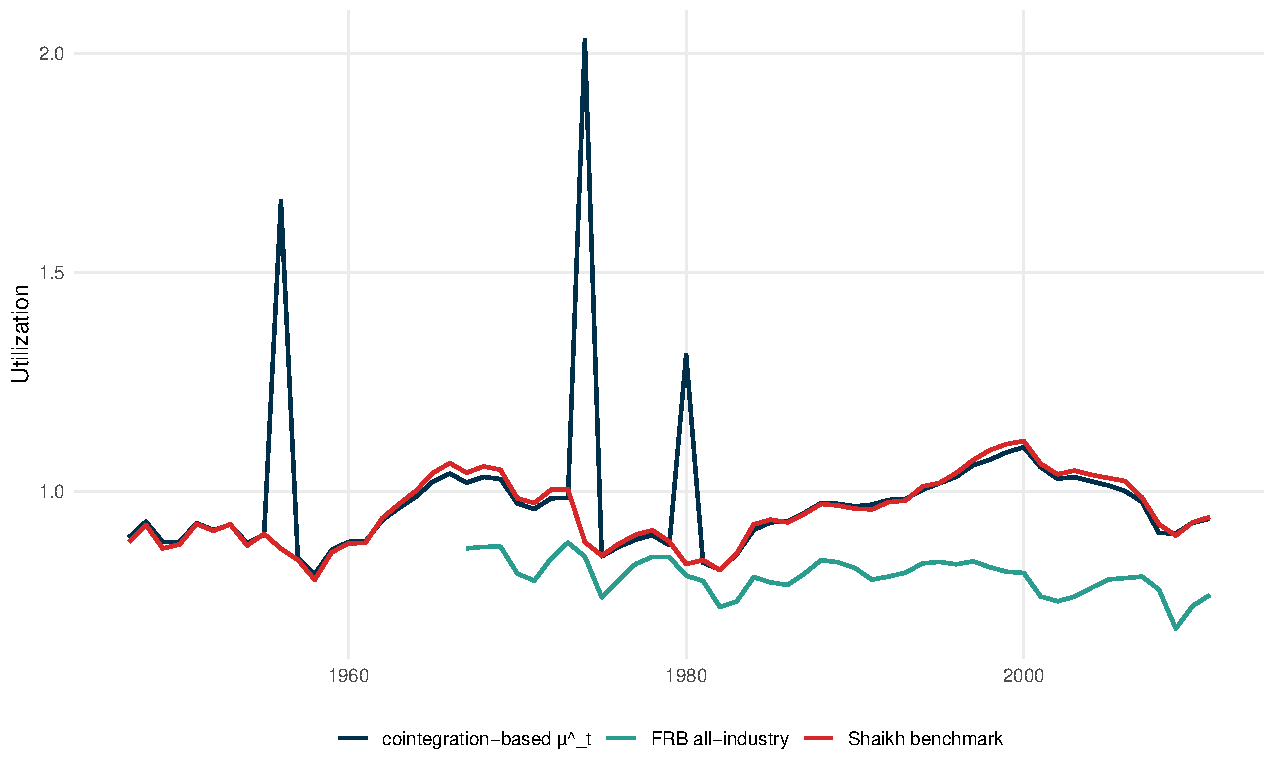
\includegraphics[width=0.85\textwidth]{appendixA/figures/fig_A10_shaikh_frb_utilization.pdf}
\caption{Capacity utilization comparison: Shaikh (cointegration-based) versus FRB survey measure, 1947--2011. Descriptive comparison only.}
\label{fig:app_utilization_comparison}
\end{figure}

% ---------------------------------------------------------------
% A.8 — ARDL Specification Search and Bounds Testing
% ---------------------------------------------------------------
\subsection{ARDL Specification Search and Bounds Testing}
\label{subsec:app_ardl_bounds}

Table~\ref{tab:app_ardl_search} displays an illustrative diagnostic subset of the specification grid ($p,q \in \{1,\dots,5\}$; Cases I--V) with information criteria, diagnostic tests, and recovered long-run coefficients. Asterisks mark case-specific AIC/BIC minima.

% ---------------------------------------------------------------
% Table A.3: ARDL Specification Search Results
% Note: Requires \usepackage{pdflscape} and \begin{landscape}...\end{landscape}
% ---------------------------------------------------------------
\begin{landscape}
\begin{longtable}[t]{rrlrrrrrrrll}
\caption{ARDL specification search: information criteria and diagnostics (1947--2011)}\label{tab:app_ardl_search}\\
\toprule
$p$ & $q$ & Case & AIC & SBC & $T_{\text{eff}}$ & $\hat{\theta}$ & LM(1) & $p$-val & LM(4) & $p$-val & Best \\
\midrule
1 & 1 & I & $-237.63$ & $-222.52$ & 64 & 0.8529 & 3.2749 & 0.070 & 5.0893 & 0.278 & \\
1 & 1 & II & $-243.09$ & $-225.82$ & 64 & 0.6989 & 3.7150 & 0.054 & 6.9003 & 0.141 & \\
1 & 1 & III & $-243.09$ & $-225.82$ & 64 & 0.6989 & 3.7150 & 0.054 & 6.9003 & 0.141 & \\
1 & 1 & IV & $-243.09$ & $-223.66$ & 64 & $-0.5048$ & 3.4486 & 0.063 & 6.5385 & 0.162 & \\
1 & 1 & V & $-243.09$ & $-223.66$ & 64 & $-0.5048$ & 3.4486 & 0.063 & 6.5385 & 0.162 & \\
\addlinespace
1 & 2 & I & $-239.33$ & $-222.19$ & 63 & 0.7273 & 7.0198 & 0.008 & 11.1845 & 0.025 & \\
1 & 2 & II & $-242.69$ & $-223.41$ & 63 & 0.7110 & 7.1117 & 0.008 & 11.8692 & 0.018 & \\
1 & 2 & III & $-242.69$ & $-223.41$ & 63 & 0.7110 & 7.1117 & 0.008 & 11.8692 & 0.018 & \\
1 & 2 & IV & $-241.90$ & $-220.47$ & 63 & $-0.4718$ & 7.0457 & 0.008 & 11.2449 & 0.024 & \\
1 & 2 & V & $-241.90$ & $-220.47$ & 63 & $-0.4718$ & 7.0457 & 0.008 & 11.2449 & 0.024 & \\
\addlinespace
1 & 3 & I & $-244.02$ & $-224.88$ & 62 & 0.8967 & 11.3499 & 0.001 & 14.1599 & 0.007 & \\
1 & 3 & II & $-249.33$ & $-228.05$ & 62 & 0.6695 & 10.3605 & 0.001 & 12.7048 & 0.013 & \\
1 & 3 & III & $-249.33$ & $-228.05$ & 62 & 0.6695 & 10.3605 & 0.001 & 12.7048 & 0.013 & \\
1 & 3 & IV & $-249.62$ & $-226.22$ & 62 & $-0.8749$ & 10.3560 & 0.001 & 11.9612 & 0.018 & * \\
1 & 3 & V & $-249.62$ & $-226.22$ & 62 & $-0.8749$ & 10.3560 & 0.001 & 11.9612 & 0.018 & * \\
\addlinespace
2 & 3 & I & $-250.91$ & $-229.63$ & 62 & 0.9301 & 5.4621 & 0.019 & 9.3503 & 0.053 & \\
2 & 3 & II & $-262.79$ & $-239.40$ & 62 & 0.7023 & 0.5641 & 0.453 & 3.5633 & 0.468 & * \\
2 & 3 & III & $-262.79$ & $-239.40$ & 62 & 0.7023 & 0.5641 & 0.453 & 3.5633 & 0.468 & * \\
2 & 3 & IV & $-264.33$ & $-238.81$ & 62 & $-0.4836$ & 0.2849 & 0.594 & 2.6102 & 0.625 & * \\
2 & 3 & V & $-264.33$ & $-238.81$ & 62 & $-0.4836$ & 0.2849 & 0.594 & 2.6102 & 0.625 & * \\
\addlinespace
4 & 5 & I & $-253.33$ & $-224.01$ & 60 & 0.7899 & 0.0461 & 0.830 & 7.6617 & 0.105 & * \\
4 & 5 & II & $-257.75$ & $-226.33$ & 60 & 0.7102 & 0.2628 & 0.608 & 6.6363 & 0.156 & \\
4 & 5 & III & $-257.75$ & $-226.33$ & 60 & 0.7102 & 0.2628 & 0.608 & 6.6363 & 0.156 & \\
4 & 5 & IV & $-257.11$ & $-223.60$ & 60 & $-0.4117$ & 0.2120 & 0.645 & 6.5141 & 0.164 & \\
4 & 5 & V & $-257.11$ & $-223.60$ & 60 & $-0.4117$ & 0.2120 & 0.645 & 6.5141 & 0.164 & \\
\bottomrule
\end{longtable}
\noindent\footnotesize\textbf{Note:} Illustrative diagnostic subset of ARDL($p,q$) specifications estimated with permanent step controls $S_{1956}, S_{1974}, S_{1980}$. AIC/SBC: Akaike/Schwarz information criteria (lower = better). $T_{\text{eff}}$: effective sample size after lag construction. $\hat{\theta}$: long-run output--capital coefficient recovered from ECM parameters. LM(1)/LM(4): Breusch--Godfrey serial correlation tests (null = no autocorrelation). Asterisk (*) marks best specification by AIC/SBC within each deterministic case. Full 500-model specification grid ($p,q \in \{1,\dots,5\}$; Cases I--V; four dummy configurations) available in replication code.
\end{landscape}

\begin{figure}[!ht]
\centering
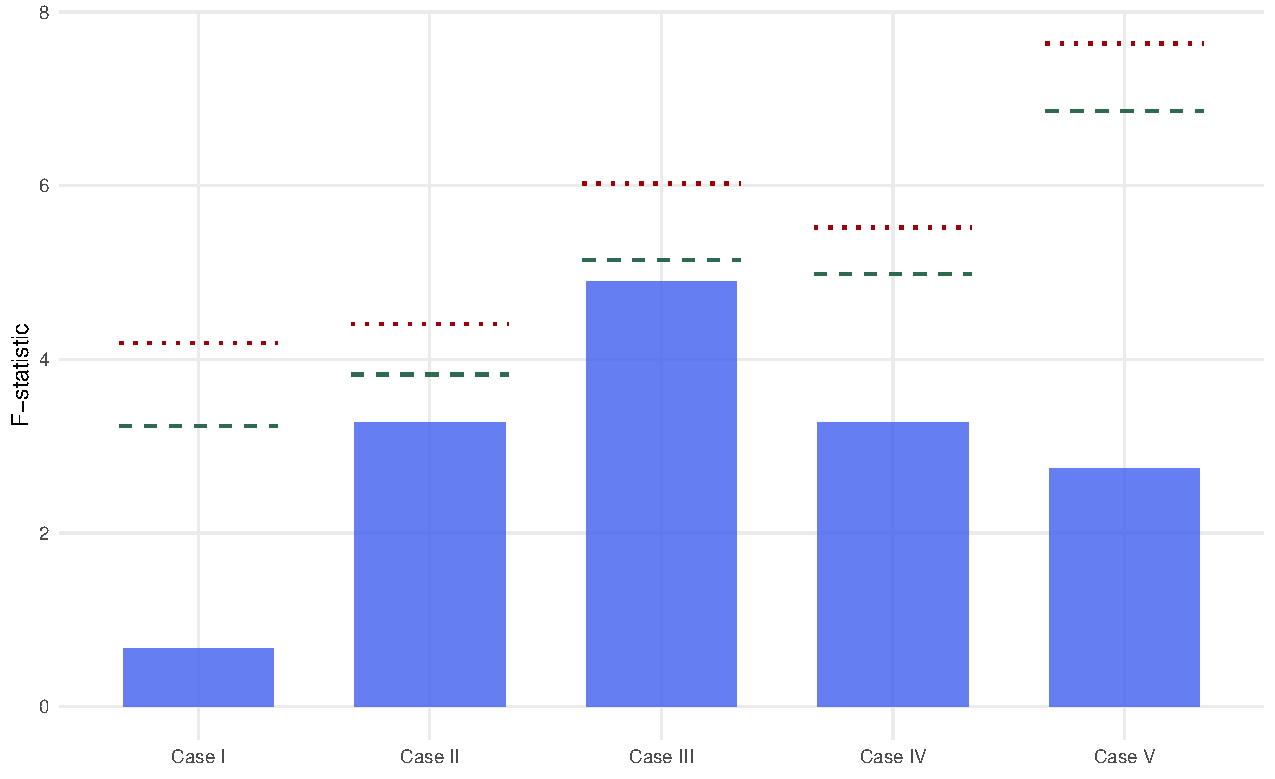
\includegraphics[width=0.85\textwidth]{appendixA/figures/fig_A11_f_bounds_cases.pdf}
\caption{$F$-statistic across deterministic Cases I--V. Horizontal lines mark lower ($I(0)$) and upper ($I(1)$) critical bounds at 5\% significance.}
\label{fig:app_f_bounds_cases}
\end{figure}

\begin{figure}[!ht]
\centering
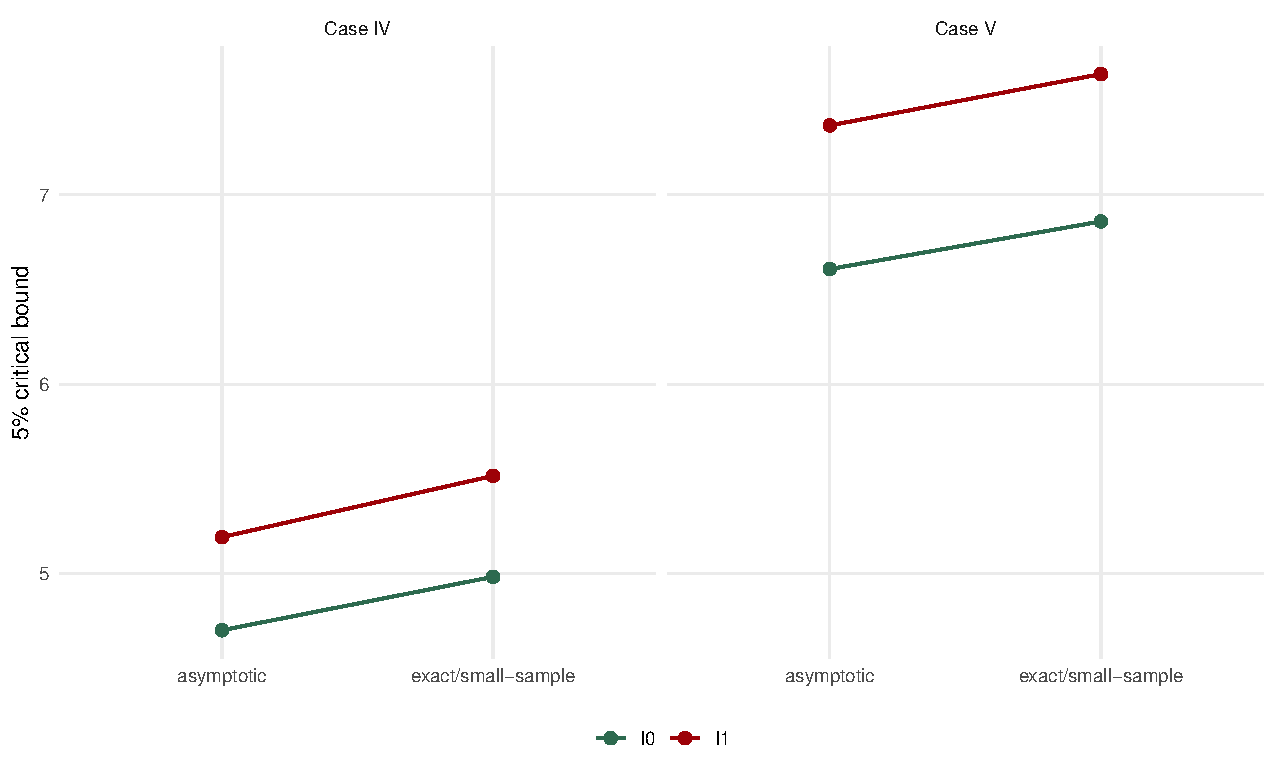
\includegraphics[width=0.85\textwidth]{appendixA/figures/fig_A12_exact_vs_asymptotic_bounds.pdf}
\caption{Exact-sample versus asymptotic critical bounds for Cases IV and V ($T=65$). Exact bounds computed via stochastic simulation \citep{NatsiopoulosTzeremes2022}.}
\label{fig:app_exact_asymptotic_bounds}
\end{figure}

\begin{figure}[!ht]
\centering
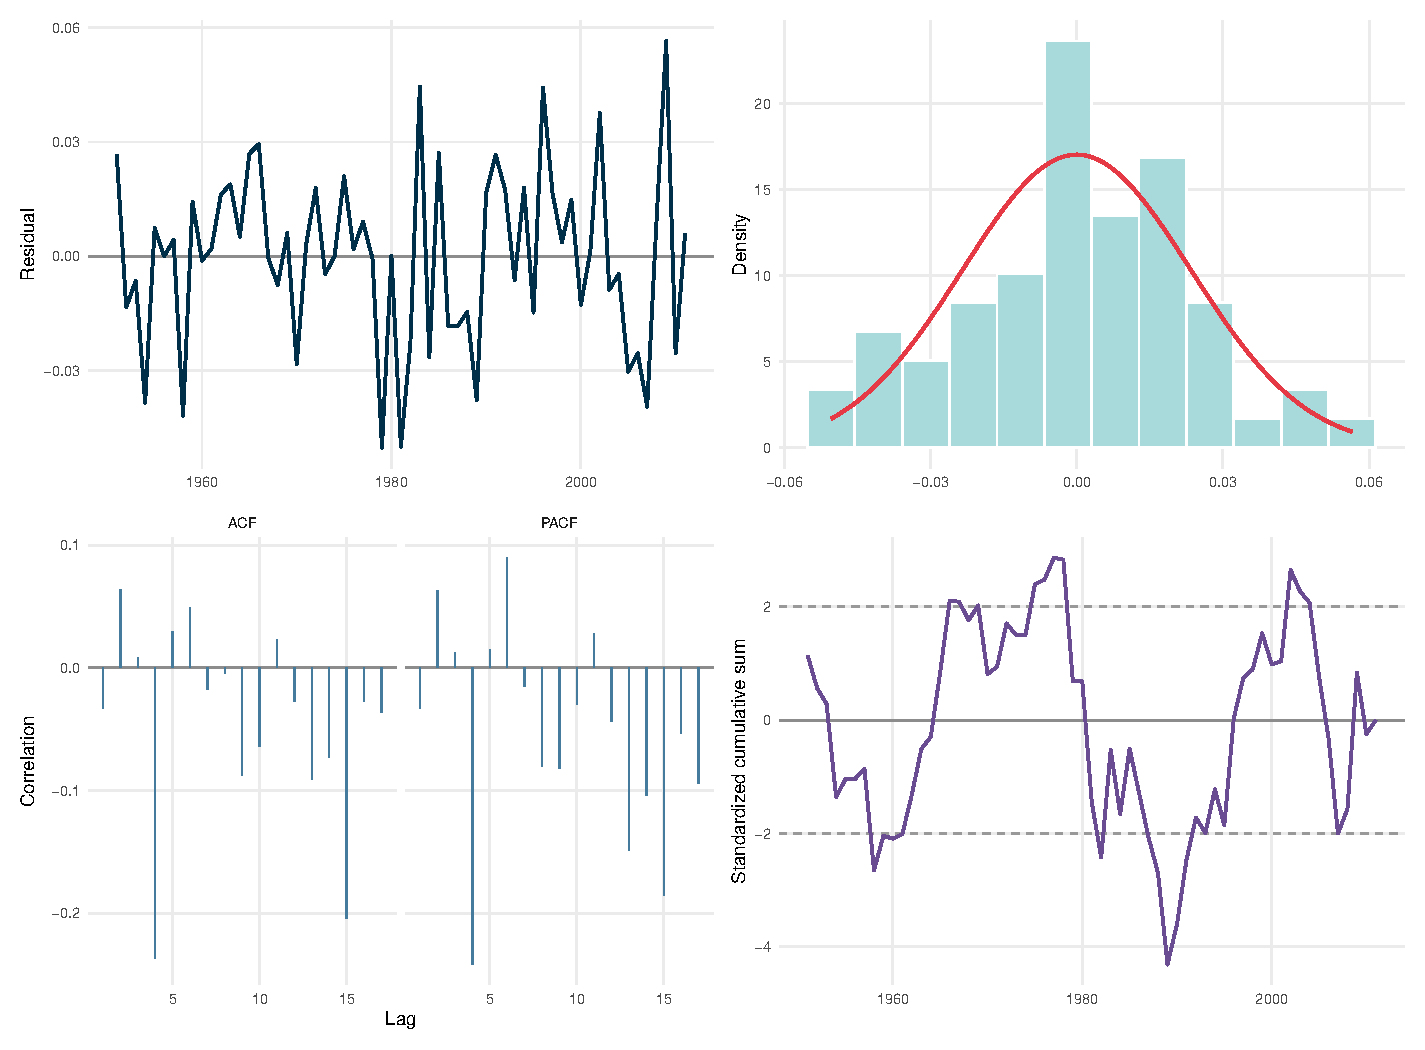
\includegraphics[width=0.85\textwidth]{appendixA/figures/fig_A13_baseline_residual_diagnostics.pdf}
\caption{Residual diagnostics from baseline ARDL(2,4): (a) residuals over time, (b) density with normal curve, (c) ACF/PACF, (d) CUSUM test.}
\label{fig:app_residual_diagnostics}
\end{figure}

\begin{figure}[!ht]
\centering
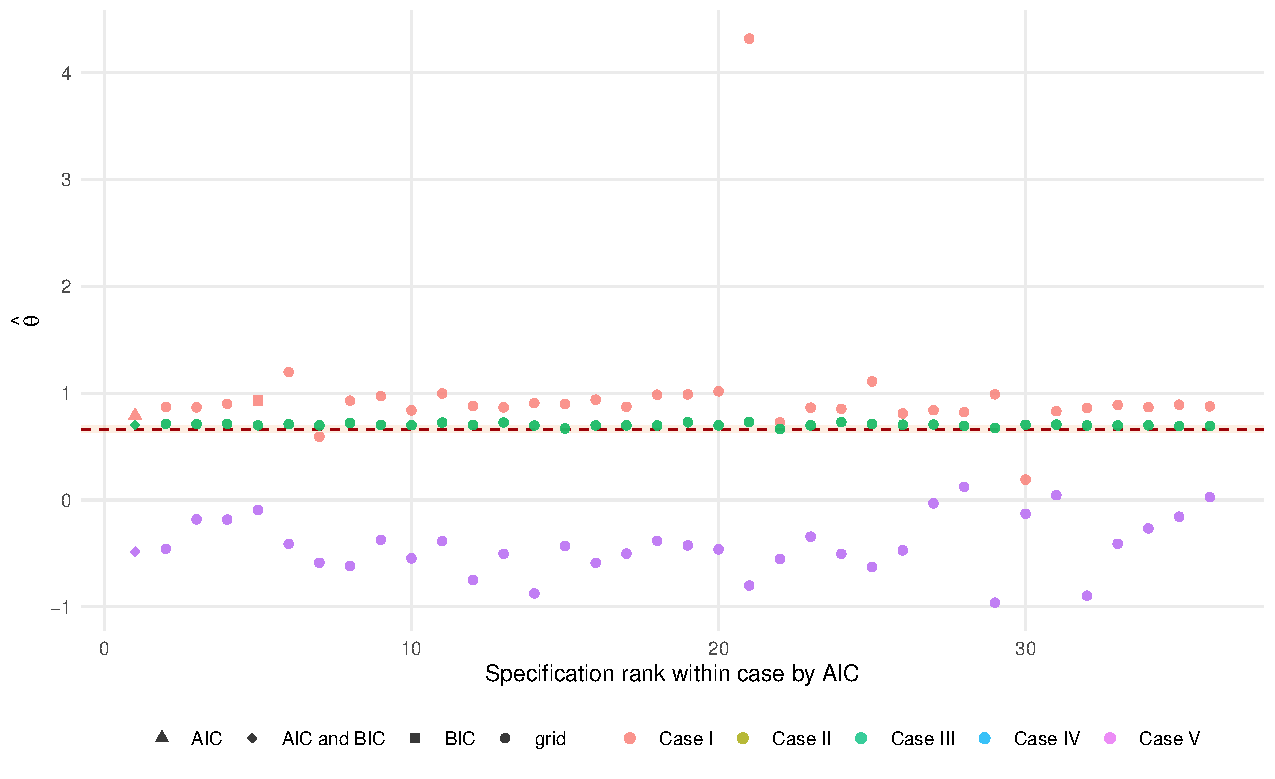
\includegraphics[width=0.85\textwidth]{appendixA/figures/fig_A14_theta_stability_grid.pdf}
\caption{Long-run coefficient $\hat{\theta}$ estimates ranked by AIC across specification grid. Horizontal band marks Shaikh's 0.6609 $\pm$ 5\%.}
\label{fig:app_theta_stability}
\end{figure}

% ---------------------------------------------------------------
% A.9 — Dummy Variable Diagnostics
% ---------------------------------------------------------------
\subsection{Dummy Variable Diagnostics}
\label{subsec:app_dummies}

Figure~\ref{fig:app_dummies_residuals} displays squared residuals from the baseline ARDL specification with pulse shock markers $P_{56}$, $P_{74}$, $P_{80}$ overlaid. These markers highlight outlier-driven residual spikes identified via squared-error diagnostics \citep{Patterson2000}, which are absorbed by permanent step indicators $S_{yy,t}$ in estimation.

\begin{figure}[!ht]
\centering
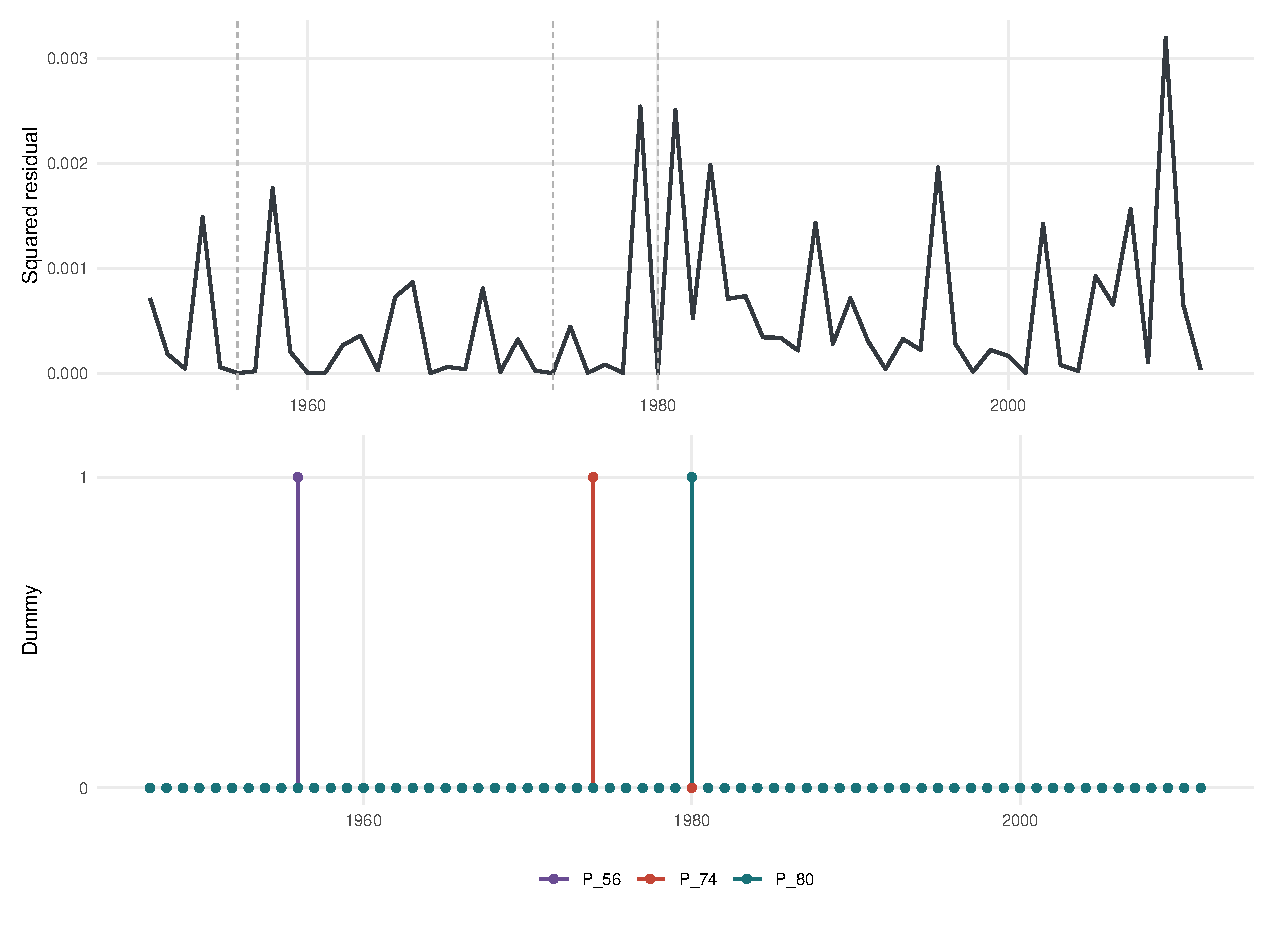
\includegraphics[width=0.85\textwidth]{appendixA/figures/fig_A5_dummies_residuals.pdf}
\caption{Squared residuals from baseline ARDL with pulse shock markers $P_{56}$, $P_{74}$, $P_{80}$ overlaid (1947--2011). Markers identify outlier-driven spikes absorbed by estimation step controls.}
\label{fig:app_dummies_residuals}
\end{figure}

% ---------------------------------------------------------------
% A.10 — Series Construction Protocol
% ---------------------------------------------------------------
\subsection{Series Construction Protocol}
\label{subsec:app_construction_flow}

Figure~\ref{fig:app_construction_flow} visualizes the pipeline from raw data to fitted capacity utilization ($\hat{\mu}_t$). The flowchart traces corrections, deflation, GPIM recursion, ARDL estimation, and residualization.

\begin{figure}[!ht]
\centering
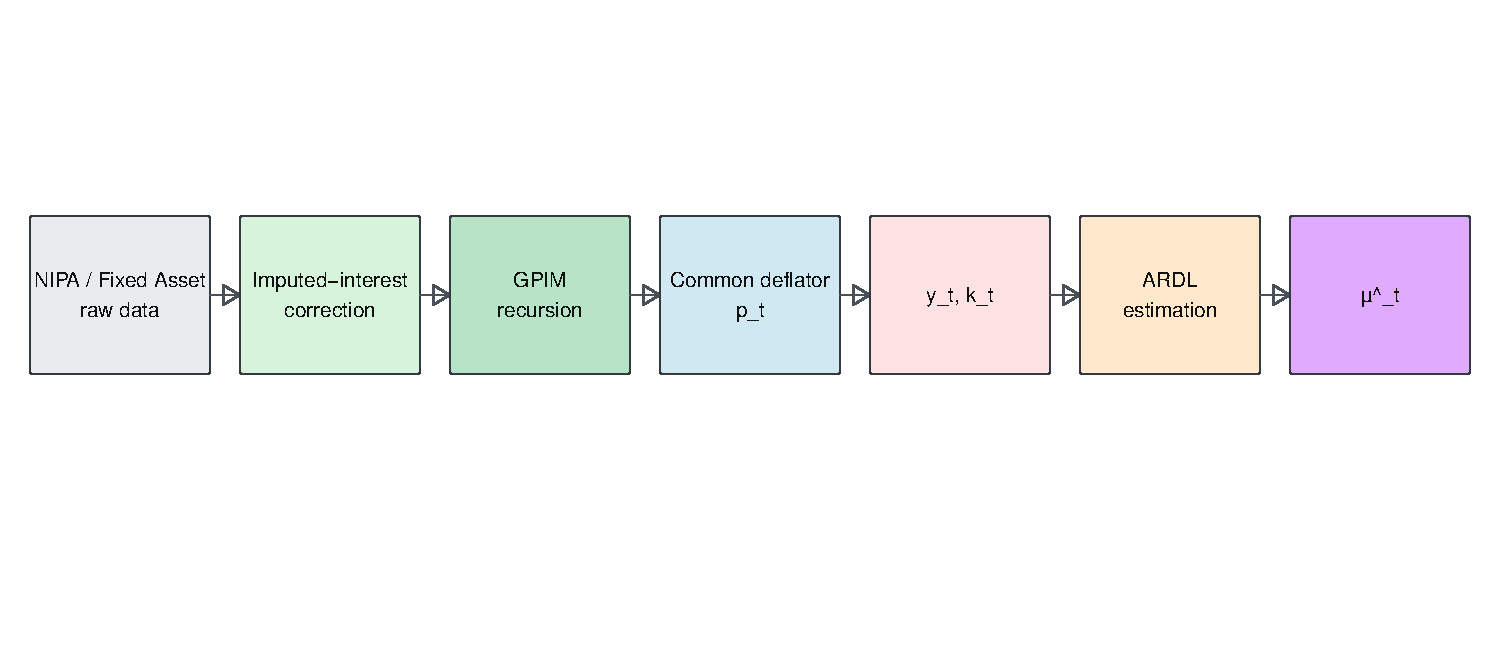
\includegraphics[width=0.85\textwidth]{appendixA/figures/fig_A15_series_construction_protocol.pdf}
\caption{Series construction protocol: raw data $\to$ corrected output/GPIM capital $\to$ common deflator $\to$ ARDL estimation $\to$ $\hat{\mu}_t$.}
\label{fig:app_construction_flow}
\end{figure}
\end{appendices}

\end{document}
